\documentclass[
%paper=5.5in:8.5in,
a5paper,
BCOR=7mm,
twoside,
DIV=calc,
11pt,
usegeometry,
chapterprefix,
endperiod,
headings=big]{scrbook} % Document font size and paper size

%\documentclass[paper=5.5in:8.5in,BCOR=15mm,twoside,DIV=calc,headinclude=off,openany]{scrbook} % Document font size and paper size

\usepackage{polyglossia}
\usepackage{graphicx}
\usepackage{lettrine}
\usepackage{xcolor}
\usepackage{fontspec}
%\usepackage[utf8]{inputenc} 
\usepackage[T1]{fontenc} % International character encodings
\usepackage{makeidx}
\usepackage{scrlayer-scrpage}
\usepackage{pifont}
\usepackage{enumitem}
\usepackage{caption}
\usepackage[maxlevel=3]{csquotes}
\usepackage[export]{adjustbox}
\usepackage{ebgaramond}
\usepackage{wrapfig}
\usepackage{afterpage}
\usepackage{setspace}
\usepackage[pass]{geometry}
\usepackage{microtype}
\usepackage[all]{nowidow}
\usepackage{subfiles}
\usepackage{floatpag}
\usepackage{pdfpages}

%\usepackage[showframe]{geometry}

\MakeAutoQuote{»}{«}
\catcode`\—=13
\protected\def—{\allowbreak\textemdash\allowbreak}
\newcommand\longdash{\mbox{---\,}\ignorespaces{}}

\floatpagestyle{empty}

\setdefaultlanguage[variant=uk]{english}
\setotherlanguage{french}
\setotherlanguage{german}
\newcommand{\HUGE}{\fontsize{50}{60}\selectfont}
\newcommand{\moderatelyhuge}{\fontsize{50}{60}\selectfont}
\newcommand{\reasonablyhuge}{\fontsize{30}{40}\selectfont}

%\newfontfamily\booktitlefont[RawFeature={-ss02},LetterSpace=40,WordSpace=6]{EB Garamond}
%\newfontfamily\spacedfont[RawFeature={-ss02},LetterSpace=20,WordSpace=3]{EB Garamond}

\input Zallman.fd
\newcommand*\initfamily{\usefont{U}{Zallman}{xl}{n}}

\setmainfont{EB Garamond}[UprightFeatures={CharacterVariant=11}]

\newfontfamily\lettrinefont{Zallman}
\renewcommand{\LettrineFontHook}{\fontspec{Zallman}}
\newfontfamily\headerfont{EB Garamond}
\newfontfamily\chapterfont{EB Garamond}

\newcount\zzc
\makeatletter
\def\zz{%
\ifnum\prevgraf<\c@L@lines
\zzc\z@
\loop
\ifnum\zzc<\prevgraf
\advance\zzc\@ne
\afterassignment\zzda\count@\L@parshape\relax
\repeat
\parshape\L@parshape
\fi}
\def\zzda{\afterassignment\zzdb\dimen@}
\def\zzdb{\afterassignment\zzdef\dimen@}
\def\zzdef#1\relax{\edef\L@parshape{\the\numexpr\count@-1\relax\space #1}}
\makeatother

\renewcommand*{\chaptermarkformat}{}
%\renewcommand*{\chapterheadendvskip}{\vspace{10pt}}
%\renewcommand*{\chapterheadstartvskip}{\vspace{0pt}}




\defaultfontfeatures{Ligatures=TeX}
%\addtokomafont{part}{libertine}
%\addtokomafont{partnumber}{libertine}
\addtokomafont{part}{ebgaramond}
\addtokomafont{partnumber}{ebgaramond}

\automark{chapter}
\lehead{The Sign of the Four}
\rohead{Chapter \thechapter: \leftmark}

\headsep=10pt
\headheight=45pt
\footskip=30pt
%\raggedbottom

\setkomafont{chapter}{\chapterfont\Huge\bfseries}
%\renewcommand*{\chaptermarkformat}{%
%
%\chapapp~\thechapter\autodot\enskip}

\hyphenation{}

\addtokomafont{disposition}{\normalfont}

\graphicspath{ {./images/} }
\captionsetup[figure]{font=sc}
\captionsetup{labelformat=empty}

\begin{document}
\KOMAoptions{headings=openany}
\renewcommand*\raggedchapter{\centering}
\thispagestyle{empty}
%\begin{figure}[p]
%\centering
%%\begin{minipage}[c]{1.2\linewidth}
%\includegraphics[width=1.1\linewidth]{frontispiece}
%%\end{minipage}
%\end{figure}
%
  \begin{titlepage}
   \includepdf[width=1.1\textwidth]{signfour.png}
  \end{titlepage}

%
%  \recalctypearea
%\restoregeometry


%\DeclareTOCStyleEntry[option list ]{style }{entry level }
%\RedeclareSectionCommand[beforeskip=0pt,afterskip=\baselineskip,innerskip=0pt,afterindent=false]{chapter}

\DeclareTOCStyleEntry[linefill=\TOCLineLeaderFill]{chapter}{chapter}

\tableofcontents
\thispagestyle{empty}



\pagestyle{headings}
\renewcommand*{\chapterpagestyle}{plain}

\KOMAoptions{headings=openright}
%!TeX root=../signtop.tex
\chapter{The Science of Deduction}
\lettrine[lines=4]{S}{herlock}  Holmes took his bottle from the corner of the mantel-piece and his hypodermic syringe from its neat morocco case. With his long, white, nervous fingers he adjusted the delicate needle, and rolled back his left shirt-cuff. For some little time his eyes rested thoughtfully upon the sinewy forearm and wrist all dotted and scarred with innumerable puncture-marks. Finally he thrust the sharp point home, pressed down the tiny piston, and sank back into the velvet-lined arm-chair with a long sigh of satisfaction.

Three times a day for many months I had witnessed this performance, but custom had not reconciled my mind to it. On the contrary, from day to day I had become more irritable at the sight, and my conscience swelled nightly within me at the thought that I had lacked the courage to protest. Again and again I had registered a vow that I should deliver my soul upon the subject, but there was that in the cool, nonchalant air of my companion which made him the last man with whom one would care to take anything approaching to a liberty. His great powers, his masterly manner, and the experience which I had had of his many extraordinary qualities, all made me diffident and backward in crossing him.

Yet upon that afternoon, whether it was the Beaune which I had taken with my lunch, or the additional exasperation produced by the extreme deliberation of his manner, I suddenly felt that I could hold out no longer.

»Which is it to-day?« I asked,—»morphine or cocaine?«

He raised his eyes languidly from the old black-letter volume which he had opened. »It is cocaine,« he said,—»a seven-per-cent. solution. Would you care to try it?«

»No, indeed,« I answered, brusquely. »My constitution has not got over the Afghan campaign yet. I cannot afford to throw any extra strain upon it.«

He smiled at my vehemence. »Perhaps you are right, Watson,« he said. »I suppose that its influence is physically a bad one. I find it, however, so transcendently stimulating and clarifying to the mind that its secondary action is a matter of small moment.«

»But consider!« I said, earnestly. »Count the cost! Your brain may, as you say, be roused and excited, but it is a pathological and morbid process, which involves increased tissue-change and may at last leave a permanent weakness. You know, too, what a black reaction comes upon you. Surely the game is hardly worth the candle. Why should you, for a mere passing pleasure, risk the loss of those great powers with which you have been endowed? Remember that I speak not only as one comrade to another, but as a medical man to one for whose constitution he is to some extent answerable.«

He did not seem offended. On the contrary, he put his finger-tips together and leaned his elbows on the arms of his chair, like one who has a relish for conversation.

»My mind,« he said, »rebels at stagnation. Give me problems, give me work, give me the most abstruse cryptogram or the most intricate analysis, and I am in my own proper atmosphere. I can dispense then with artificial stimulants. But I abhor the dull routine of existence. I crave for mental exaltation. That is why I have chosen my own particular profession,—or rather created it, for I am the only one in the world.«

»The only unofficial detective?« I said, raising my eyebrows.

»The only unofficial consulting detective,« he answered. »I am the last and highest court of appeal in detection. When Gregson or Lestrade or Athelney Jones are out of their depths—which, by the way, is their normal state—the matter is laid before me. I examine the data, as an expert, and pronounce a specialist's opinion. I claim no credit in such cases. My name figures in no newspaper. The work itself, the pleasure of finding a field for my peculiar powers, is my highest reward. But you have yourself had some experience of my methods of work in the Jefferson Hope case.«

»Yes, indeed,« said I, cordially. »I was never so struck by anything in my life. I even embodied it in a small brochure with the somewhat fantastic title of »A Study in Scarlet.««

He shook his head sadly. »I glanced over it,« said he. »Honestly, I cannot congratulate you upon it. Detection is, or ought to be, an exact science, and should be treated in the same cold and unemotional manner. You have attempted to tinge it with romanticism, which produces much the same effect as if you worked a love-story or an elopement into the fifth proposition of Euclid.«

»But the romance was there,« I remonstrated. »I could not tamper with the facts.«

»Some facts should be suppressed, or at least a just sense of proportion should be observed in treating them. The only point in the case which deserved mention was the curious analytical reasoning from effects to causes by which I succeeded in unravelling it.«

I was annoyed at this criticism of a work which had been specially designed to please him. I confess, too, that I was irritated by the egotism which seemed to demand that every line of my pamphlet should be devoted to his own special doings. More than once during the years that I had lived with him in Baker Street I had observed that a small vanity underlay my companion's quiet and didactic manner. I made no remark, however, but sat nursing my wounded leg. I had a Jezail bullet through it some time before, and, though it did not prevent me from walking, it ached wearily at every change of the weather.

»My practice has extended recently to the Continent,« said Holmes, after a while, filling up his old brier-root pipe. »I was consulted last week by François Le Villard, who, as you probably know, has come rather to the front lately in the French detective service. He has all the Celtic power of quick intuition, but he is deficient in the wide range of exact knowledge which is essential to the higher developments of his art. The case was concerned with a will, and possessed some features of interest. I was able to refer him to two parallel cases, the one at Riga in 1857, and the other at St Louis in 1871, which have suggested to him the true solution. Here is the letter which I had this morning acknowledging my assistance.« He tossed over, as he spoke, a crumpled sheet of foreign notepaper. I glanced my eyes down it, catching a profusion of notes of admiration, with stray »magnifiques,« »coup-de-maîtres,« and »tours-de-force,« all testifying to the ardent admiration of the Frenchman.

»He speaks as a pupil to his master,« said I.

»Oh, he rates my assistance too highly,« said Sherlock Holmes, lightly. »He has considerable gifts himself. He possesses two out of the three qualities necessary for the ideal detective. He has the power of observation and that of deduction. He is only wanting in knowledge; and that may come in time. He is now translating my small works into French.«

»Your works?«

»Oh, didn't you know?« he cried, laughing. »Yes, I have been guilty of several monographs. They are all upon technical subjects. Here, for example, is one »Upon the Distinction between the Ashes of the Various Tobaccoes.« In it I enumerate a hundred and forty forms of cigar-, cigarette-, and pipe-tobacco, with coloured plates illustrating the difference in the ash. It is a point which is continually turning up in criminal trials, and which is sometimes of supreme importance as a clue. If you can say definitely, for example, that some murder has been done by a man who was smoking an Indian lunkah, it obviously narrows your field of search. To the trained eye there is as much difference between the black ash of a Trichinopoly and the white fluff of bird's-eye as there is between a cabbage and a potato.«

»You have an extraordinary genius for minutiæ,« I remarked.

»I appreciate their importance. Here is my monograph upon the tracing of footsteps, with some remarks upon the uses of plaster of Paris as a preserver of impresses. Here, too, is a curious little work upon the influence of a trade upon the form of the hand, with lithotypes of the hands of slaters, sailors, corkcutters, compositors, weavers, and diamond-polishers. That is a matter of great practical interest to the scientific detective,—especially in cases of unclaimed bodies, or in discovering the antecedents of criminals. But I weary you with my hobby.«

»Not at all,« I answered, earnestly. »It is of the greatest interest to me, especially since I have had the opportunity of observing your practical application of it. But you spoke just now of observation and deduction. Surely the one to some extent implies the other.«

»Why, hardly,« he answered, leaning back luxuriously in his arm-chair, and sending up thick blue wreaths from his pipe. »For example, observation shows me that you have been to the Wigmore Street Post-Office this morning, but deduction lets me know that when there you dispatched a telegram.«

»Right!« said I. »Right on both points! But I confess that I don't see how you arrived at it. It was a sudden impulse upon my part, and I have mentioned it to no one.«

»It is simplicity itself,« he remarked, chuckling at my surprise,—»so absurdly simple that an explanation is superfluous; and yet it may serve to define the limits of observation and of deduction. Observation tells me that you have a little reddish mould adhering to your instep. Just opposite the Wigmore Street Office they have taken up the pavement and thrown up some earth which lies in such a way that it is difficult to avoid treading in it in entering. The earth is of this peculiar reddish tint which is found, as far as I know, nowhere else in the neighbourhood. So much is observation. The rest is deduction.«

»How, then, did you deduce the telegram?«

»Why, of course I knew that you had not written a letter, since I sat opposite to you all morning. I see also in your open desk there that you have a sheet of stamps and a thick bundle of post-cards. What could you go into the post-office for, then, but to send a wire? Eliminate all other factors, and the one which remains must be the truth.«

»In this case it certainly is so,« I replied, after a little thought. »The thing, however, is, as you say, of the simplest. Would you think me impertinent if I were to put your theories to a more severe test?«

»On the contrary,« he answered, »it would prevent me from taking a second dose of cocaine. I should be delighted to look into any problem which you might submit to me.«

»I have heard you say that it is difficult for a man to have any object in daily use without leaving the impress of his individuality upon it in such a way that a trained observer might read it. Now, I have here a watch which has recently come into my possession. Would you have the kindness to let me have an opinion upon the character or habits of the late owner?«

I handed him over the watch with some slight feeling of amusement in my heart, for the test was, as I thought, an impossible one, and I intended it as a lesson against the somewhat dogmatic tone which he occasionally assumed. He balanced the watch in his hand, gazed hard at the dial, opened the back, and examined the works, first with his naked eyes and then with a powerful convex lens. I could hardly keep from smiling at his crestfallen face when he finally snapped the case to and handed it back.

»There are hardly any data,« he remarked. »The watch has been recently cleaned, which robs me of my most suggestive facts.«

»You are right,« I answered. »It was cleaned before being sent to me.« In my heart I accused my companion of putting forward a most lame and impotent excuse to cover his failure. What data could he expect from an uncleaned watch?

»Though unsatisfactory, my research has not been entirely barren,« he observed, staring up at the ceiling with dreamy, lack-lustre eyes. »Subject to your correction, I should judge that the watch belonged to your elder brother, who inherited it from your father.«

»That you gather, no doubt, from the \textsc{h.w.} upon the back?«

»Quite so. The \textsc{w.} suggests your own name. The date of the watch is nearly fifty years back, and the initials are as old as the watch: so it was made for the last generation. Jewellery usually descends to the eldest son, and he is most likely to have the same name as the father. Your father has, if I remember right, been dead many years. It has, therefore, been in the hands of your eldest brother.«

»Right, so far,« said I. »Anything else?«

»He was a man of untidy habits,—very untidy and careless. He was left with good prospects, but he threw away his chances, lived for some time in poverty with occasional short intervals of prosperity, and finally, taking to drink, he died. That is all I can gather.«

I sprang from my chair and limped impatiently about the room with considerable bitterness in my heart.

»This is unworthy of you, Holmes,« I said. »I could not have believed that you would have descended to this. You have made inquires into the history of my unhappy brother, and you now pretend to deduce this knowledge in some fanciful way. You cannot expect me to believe that you have read all this from his old watch! It is unkind, and, to speak plainly, has a touch of charlatanism in it.«

»My dear doctor,« said he, kindly, »pray accept my apologies. Viewing the matter as an abstract problem, I had forgotten how personal and painful a thing it might be to you. I assure you, however, that I never even knew that you had a brother until you handed me the watch.«

»Then how in the name of all that is wonderful did you get these facts? They are absolutely correct in every particular.«

»Ah, that is good luck. I could only say what was the balance of probability. I did not at all expect to be so accurate.«

»But it was not mere guess-work?«

»No, no: I never guess. It is a shocking habit,—destructive to the logical faculty. What seems strange to you is only so because you do not follow my train of thought or observe the small facts upon which large inferences may depend. For example, I began by stating that your brother was careless. When you observe the lower part of that watch-case you notice that it is not only dinted in two places, but it is cut and marked all over from the habit of keeping other hard objects, such as coins or keys, in the same pocket. Surely it is no great feat to assume that a man who treats a fifty-guinea watch so cavalierly must be a careless man. Neither is it a very far-fetched inference that a man who inherits one article of such value is pretty well provided for in other respects.«

I nodded, to show that I followed his reasoning.

»It is very customary for pawnbrokers in England, when they take a watch, to scratch the number of the ticket with a pin-point upon the inside of the case. It is more handy than a label, as there is no risk of the number being lost or transposed. There are no less than four such numbers visible to my lens on the inside of this case. Inference,—that your brother was often at low water. Secondary inference,—that he had occasional bursts of prosperity, or he could not have redeemed the pledge. Finally, I ask you to look at the inner plate, which contains the key-hole. Look at the thousands of scratches all round the hole,—marks where the key has slipped. What sober man's key could have scored those grooves? But you will never see a drunkard's watch without them. He winds it at night, and he leaves these traces of his unsteady hand. Where is the mystery in all this?«

»It is as clear as daylight,« I answered. »I regret the injustice which I did you. I should have had more faith in your marvellous faculty. May I ask whether you have any professional inquiry on foot at present?«

»None. Hence the cocaine. I cannot live without brain-work. What else is there to live for? Stand at the window here. Was ever such a dreary, dismal, unprofitable world? See how the yellow fog swirls down the street and drifts across the dun-coloured houses. What could be more hopelessly prosaic and material? What is the use of having powers, doctor, when one has no field upon which to exert them? Crime is commonplace, existence is commonplace, and no qualities save those which are commonplace have any function upon earth.«

I had opened my mouth to reply to this tirade, when with a crisp knock our landlady entered, bearing a card upon the brass salver.

»A young lady for you, sir,« she said, addressing my companion.

»Miss Mary Morstan,« he read. »Hum! I have no recollection of the name. Ask the young lady to step up, Mrs Hudson. Don't go, doctor. I should prefer that you remain.«
%!TeX root=../signtop.tex
\chapter{The Statement of the Case}
\lettrine[lines=4]{M}{iss} Morstan entered the room with a firm step and an outward composure of manner. She was a blonde young lady, small, dainty, well gloved, and dressed in the most perfect taste. There was, however, a plainness and simplicity about her costume which bore with it a suggestion of limited means. The dress was a sombre greyish beige, untrimmed and unbraided, and she wore a small turban of the same dull hue, relieved only by a suspicion of white feather in the side. Her face had neither regularity of feature nor beauty of complexion, but her expression was sweet and amiable, and her large blue eyes were singularly spiritual and sympathetic. In an experience of women which extends over many nations and three separate continents, I have never looked upon a face which gave a clearer promise of a refined and sensitive nature. I could not but observe that as she took the seat which Sherlock Holmes placed for her, her lip trembled, her hand quivered, and she showed every sign of intense inward agitation.

»I have come to you, Mr Holmes,« she said, »because you once enabled my employer, Mrs Cecil Forrester, to unravel a little domestic complication. She was much impressed by your kindness and skill.«

»Mrs Cecil Forrester,« he repeated thoughtfully. »I believe that I was of some slight service to her. The case, however, as I remember it, was a very simple one.«

»She did not think so. But at least you cannot say the same of mine. I can hardly imagine anything more strange, more utterly inexplicable, than the situation in which I find myself.«

Holmes rubbed his hands, and his eyes glistened. He leaned forward in his chair with an expression of extraordinary concentration upon his clear-cut, hawklike features. »State your case,« said he, in brisk, business tones.

I felt that my position was an embarrassing one. »You will, I am sure, excuse me,« I said, rising from my chair.

To my surprise, the young lady held up her gloved hand to detain me. »If your friend,« she said, »would be good enough to stop, he might be of inestimable service to me.«

I relapsed into my chair.

»Briefly,« she continued, »the facts are these. My father was an officer in an Indian regiment who sent me home when I was quite a child. My mother was dead, and I had no relative in England. I was placed, however, in a comfortable boarding establishment at Edinburgh, and there I remained until I was seventeen years of age. In the year 1878 my father, who was senior captain of his regiment, obtained twelve months' leave and came home. He telegraphed to me from London that he had arrived all safe, and directed me to come down at once, giving the Langham Hotel as his address. His message, as I remember, was full of kindness and love. On reaching London I drove to the Langham, and was informed that Captain Morstan was staying there, but that he had gone out the night before and had not yet returned. I waited all day without news of him. That night, on the advice of the manager of the hotel, I communicated with the police, and next morning we advertised in all the papers. Our inquiries led to no result; and from that day to this no word has ever been heard of my unfortunate father. He came home with his heart full of hope, to find some peace, some comfort, and instead\longdash« She put her hand to her throat, and a choking sob cut short the sentence.

»The date?« asked Holmes, opening his note-book.

»He disappeared upon the 3\textsuperscript{rd} of December, 1878,—nearly ten years ago.«

»His luggage?«

»Remained at the hotel. There was nothing in it to suggest a clue,—some clothes, some books, and a considerable number of curiosities from the Andaman Islands. He had been one of the officers in charge of the convict-guard there.«

»Had he any friends in town?«

»Only one that we know of,—Major Sholto, of his own regiment, the 34\textsuperscript{th} Bombay Infantry. The major had retired some little time before, and lived at Upper Norwood. We communicated with him, of course, but he did not even know that his brother officer was in England.«

»A singular case,« remarked Holmes.

»I have not yet described to you the most singular part. About six years ago—to be exact, upon the 4\textsuperscript{th} of May, 1882—an advertisement appeared in the \textit{Times} asking for the address of Miss Mary Morstan and stating that it would be to her advantage to come forward. There was no name or address appended. I had at that time just entered the family of Mrs Cecil Forrester in the capacity of governess. By her advice I published my address in the advertisement column. The same day there arrived through the post a small card-board box addressed to me, which I found to contain a very large and lustrous pearl. No word of writing was enclosed. Since then every year upon the same date there has always appeared a similar box, containing a similar pearl, without any clue as to the sender. They have been pronounced by an expert to be of a rare variety and of considerable value. You can see for yourselves that they are very handsome.« She opened a flat box as she spoke, and showed me six of the finest pearls that I had ever seen.

»Your statement is most interesting,« said Sherlock Holmes. »Has anything else occurred to you?«

»Yes, and no later than to-day. That is why I have come to you. This morning I received this letter, which you will perhaps read for yourself.«

»Thank you,« said Holmes. »The envelope too, please. Postmark, London, S.W. Date, July 7. Hum! Man's thumb-mark on corner,—probably postman. Best quality paper. Envelopes at sixpence a packet. Particular man in his stationery. No address. »Be at the third pillar from the left outside the Lyceum Theatre to-night at seven o'clock. If you are distrustful, bring two friends. You are a wronged woman, and shall have justice. Do not bring police. If you do, all will be in vain. Your unknown friend.« Well, really, this is a very pretty little mystery. What do you intend to do, Miss Morstan?«

»That is exactly what I want to ask you.«

»Then we shall most certainly go. You and I and—yes, why, Dr Watson is the very man. Your correspondent says two friends. He and I have worked together before.«

»But would he come?« she asked, with something appealing in her voice and expression.

»I should be proud and happy,« said I, fervently, »if I can be of any service.«

»You are both very kind,« she answered. »I have led a retired life, and have no friends whom I could appeal to. If I am here at six it will do, I suppose?«

»You must not be later,« said Holmes. »There is one other point, however. Is this handwriting the same as that upon the pearl-box addresses?«

»I have them here,« she answered, producing half a dozen pieces of paper.

»You are certainly a model client. You have the correct intuition. Let us see, now.« He spread out the papers upon the table, and gave little darting glances from one to the other. »They are disguised hands, except the letter,« he said, presently, »but there can be no question as to the authorship. See how the irrepressible Greek \textit{e} will break out, and see the twirl of the final \textit{s}. They are undoubtedly by the same person. I should not like to suggest false hopes, Miss Morstan, but is there any resemblance between this hand and that of your father?«

»Nothing could be more unlike.«

»I expected to hear you say so. We shall look out for you, then, at six. Pray allow me to keep the papers. I may look into the matter before then. It is only half-past three. \textit{Au revoir,} then.«

»\textit{Au revoir,}« said our visitor, and, with a bright, kindly glance from one to the other of us, she replaced her pearl-box in her bosom and hurried away. Standing at the window, I watched her walking briskly down the street, until the grey turban and white feather were but a speck in the sombre crowd.

»What a very attractive woman!« I exclaimed, turning to my companion.

He had lit his pipe again, and was leaning back with drooping eyelids. »Is she?« he said, languidly. »I did not observe.«

»You really are an automaton,—a calculating-machine!« I cried. »There is something positively inhuman in you at times.«

He smiled gently. »It is of the first importance,« he said, »not to allow your judgment to be biased by personal qualities. A client is to me a mere unit,—a factor in a problem. The emotional qualities are antagonistic to clear reasoning. I assure you that the most winning woman I ever knew was hanged for poisoning three little children for their insurance-money, and the most repellent man of my acquaintance is a philanthropist who has spent nearly a quarter of a million upon the London poor.«

»In this case, however\longdash«

»I never make exceptions. An exception disproves the rule. Have you ever had occasion to study character in handwriting? What do you make of this fellow's scribble?«

»It is legible and regular,« I answered. »A man of business habits and some force of character.«

Holmes shook his head. »Look at his long letters,« he said. »They hardly rise above the common herd. That \textit{d} might be an \textit{a}, and that \textit{l} an \textit{e}. Men of character always differentiate their long letters, however illegibly they may write. There is vacillation in his \textit{k}'s and self-esteem in his capitals. I am going out now. I have some few references to make. Let me recommend this book,—one of the most remarkable ever penned. It is Winwood Reade's \textit{Martyrdom of Man}. I shall be back in an hour.«

I sat in the window with the volume in my hand, but my thoughts were far from the daring speculations of the writer. My mind ran upon our late visitor,—her smiles, the deep rich tones of her voice, the strange mystery which overhung her life. If she were seventeen at the time of her father's disappearance she must be seven-and-twenty now,—a sweet age, when youth has lost its self-consciousness and become a little sobered by experience. So I sat and mused, until such dangerous thoughts came into my head that I hurried away to my desk and plunged furiously into the latest treatise upon pathology. What was I, an army surgeon with a weak leg and a weaker banking-account, that I should dare to think of such things? She was a unit, a factor,—nothing more. If my future were black, it was better surely to face it like a man than to attempt to brighten it by mere will-o'-the-wisps of the imagination.
%!TeX root=../houndtop.tex
\chapter{The Problem}
\lettrine[lines=1]{I}{} confess at these words a shudder passed through me. There was a thrill in the doctor's voice which showed that he was himself deeply moved by that which he told us. Holmes leaned forward in his excitement and his eyes had the hard, dry glitter which shot from them when he was keenly interested.

\enquote{You saw this?}

\enquote{As clearly as I see you.}

\enquote{And you said nothing?}

\enquote{What was the use?}

\enquote{How was it that no one else saw it?}

\enquote{The marks were some twenty yards from the body and no one gave them a thought. I don't suppose I should have done so had I not known this legend.}

\enquote{There are many sheep-dogs on the moor?}

\enquote{No doubt, but this was no sheep-dog.}

\enquote{You say it was large?}

\enquote{Enormous.}

\enquote{But it had not approached the body?}

\enquote{No.}

\enquote{What sort of night was it?}

\enquote{Damp and raw.}

\enquote{But not actually raining?}

\enquote{No.}

\enquote{What is the Alley like?}

\enquote{There are two lines of old yew hedge, twelve feet high and impenetrable. The walk in the centre is about eight feet across.}

\enquote{Is there anything between the hedges and the walk?}

\enquote{Yes, there is a strip of grass about six feet broad on either side.}

\enquote{I understand that the yew hedge is penetrated at one point by a gate?}

\enquote{Yes, the wicket-gate which leads on to the moor.}

\enquote{Is there any other opening?}

\enquote{None.}

\enquote{So that to reach the Yew Alley one either has to come down it from the house or else to enter it by the moor-gate?}

\enquote{There is an exit through a summer-house at the far end.}

\enquote{Had Sir Charles reached this?}

\enquote{No; he lay about fifty yards from it.}

\enquote{Now, tell me, Dr Mortimer---and this is important---the marks which you saw were on the path and not on the grass?}

\enquote{No marks could show on the grass.}

\enquote{Were they on the same side of the path as the moor-gate?}

\enquote{Yes; they were on the edge of the path on the same side as the moor-gate.}

\enquote{You interest me exceedingly. Another point. Was the wicket-gate closed?}

\enquote{Closed and padlocked.}

\enquote{How high was it?}

\enquote{About four feet high.}

\enquote{Then anyone could have got over it?}

\enquote{Yes.}

\enquote{And what marks did you see by the wicket-gate?}

\enquote{None in particular.}

\enquote{Good heaven! Did no one examine?}

\enquote{Yes, I examined myself.}

\enquote{And found nothing?}

\enquote{It was all very confused. Sir Charles had evidently stood there for five or ten minutes.}

\enquote{How do you know that?}

\enquote{Because the ash had twice dropped from his cigar.}

\enquote{Excellent! This is a colleague, Watson, after our own heart. But the marks?}

\enquote{He had left his own marks all over that small patch of gravel. I could discern no others.}

Sherlock Holmes struck his hand against his knee with an impatient gesture.

\enquote{If I had only been there!} he cried. \enquote{It is evidently a case of extraordinary interest, and one which presented immense opportunities to the scientific expert. That gravel page upon which I might have read so much has been long ere this smudged by the rain and defaced by the clogs of curious peasants. Oh, Dr Mortimer, Dr Mortimer, to think that you should not have called me in! You have indeed much to answer for.}

%\begin{figure}[tbhp]
%\centering
%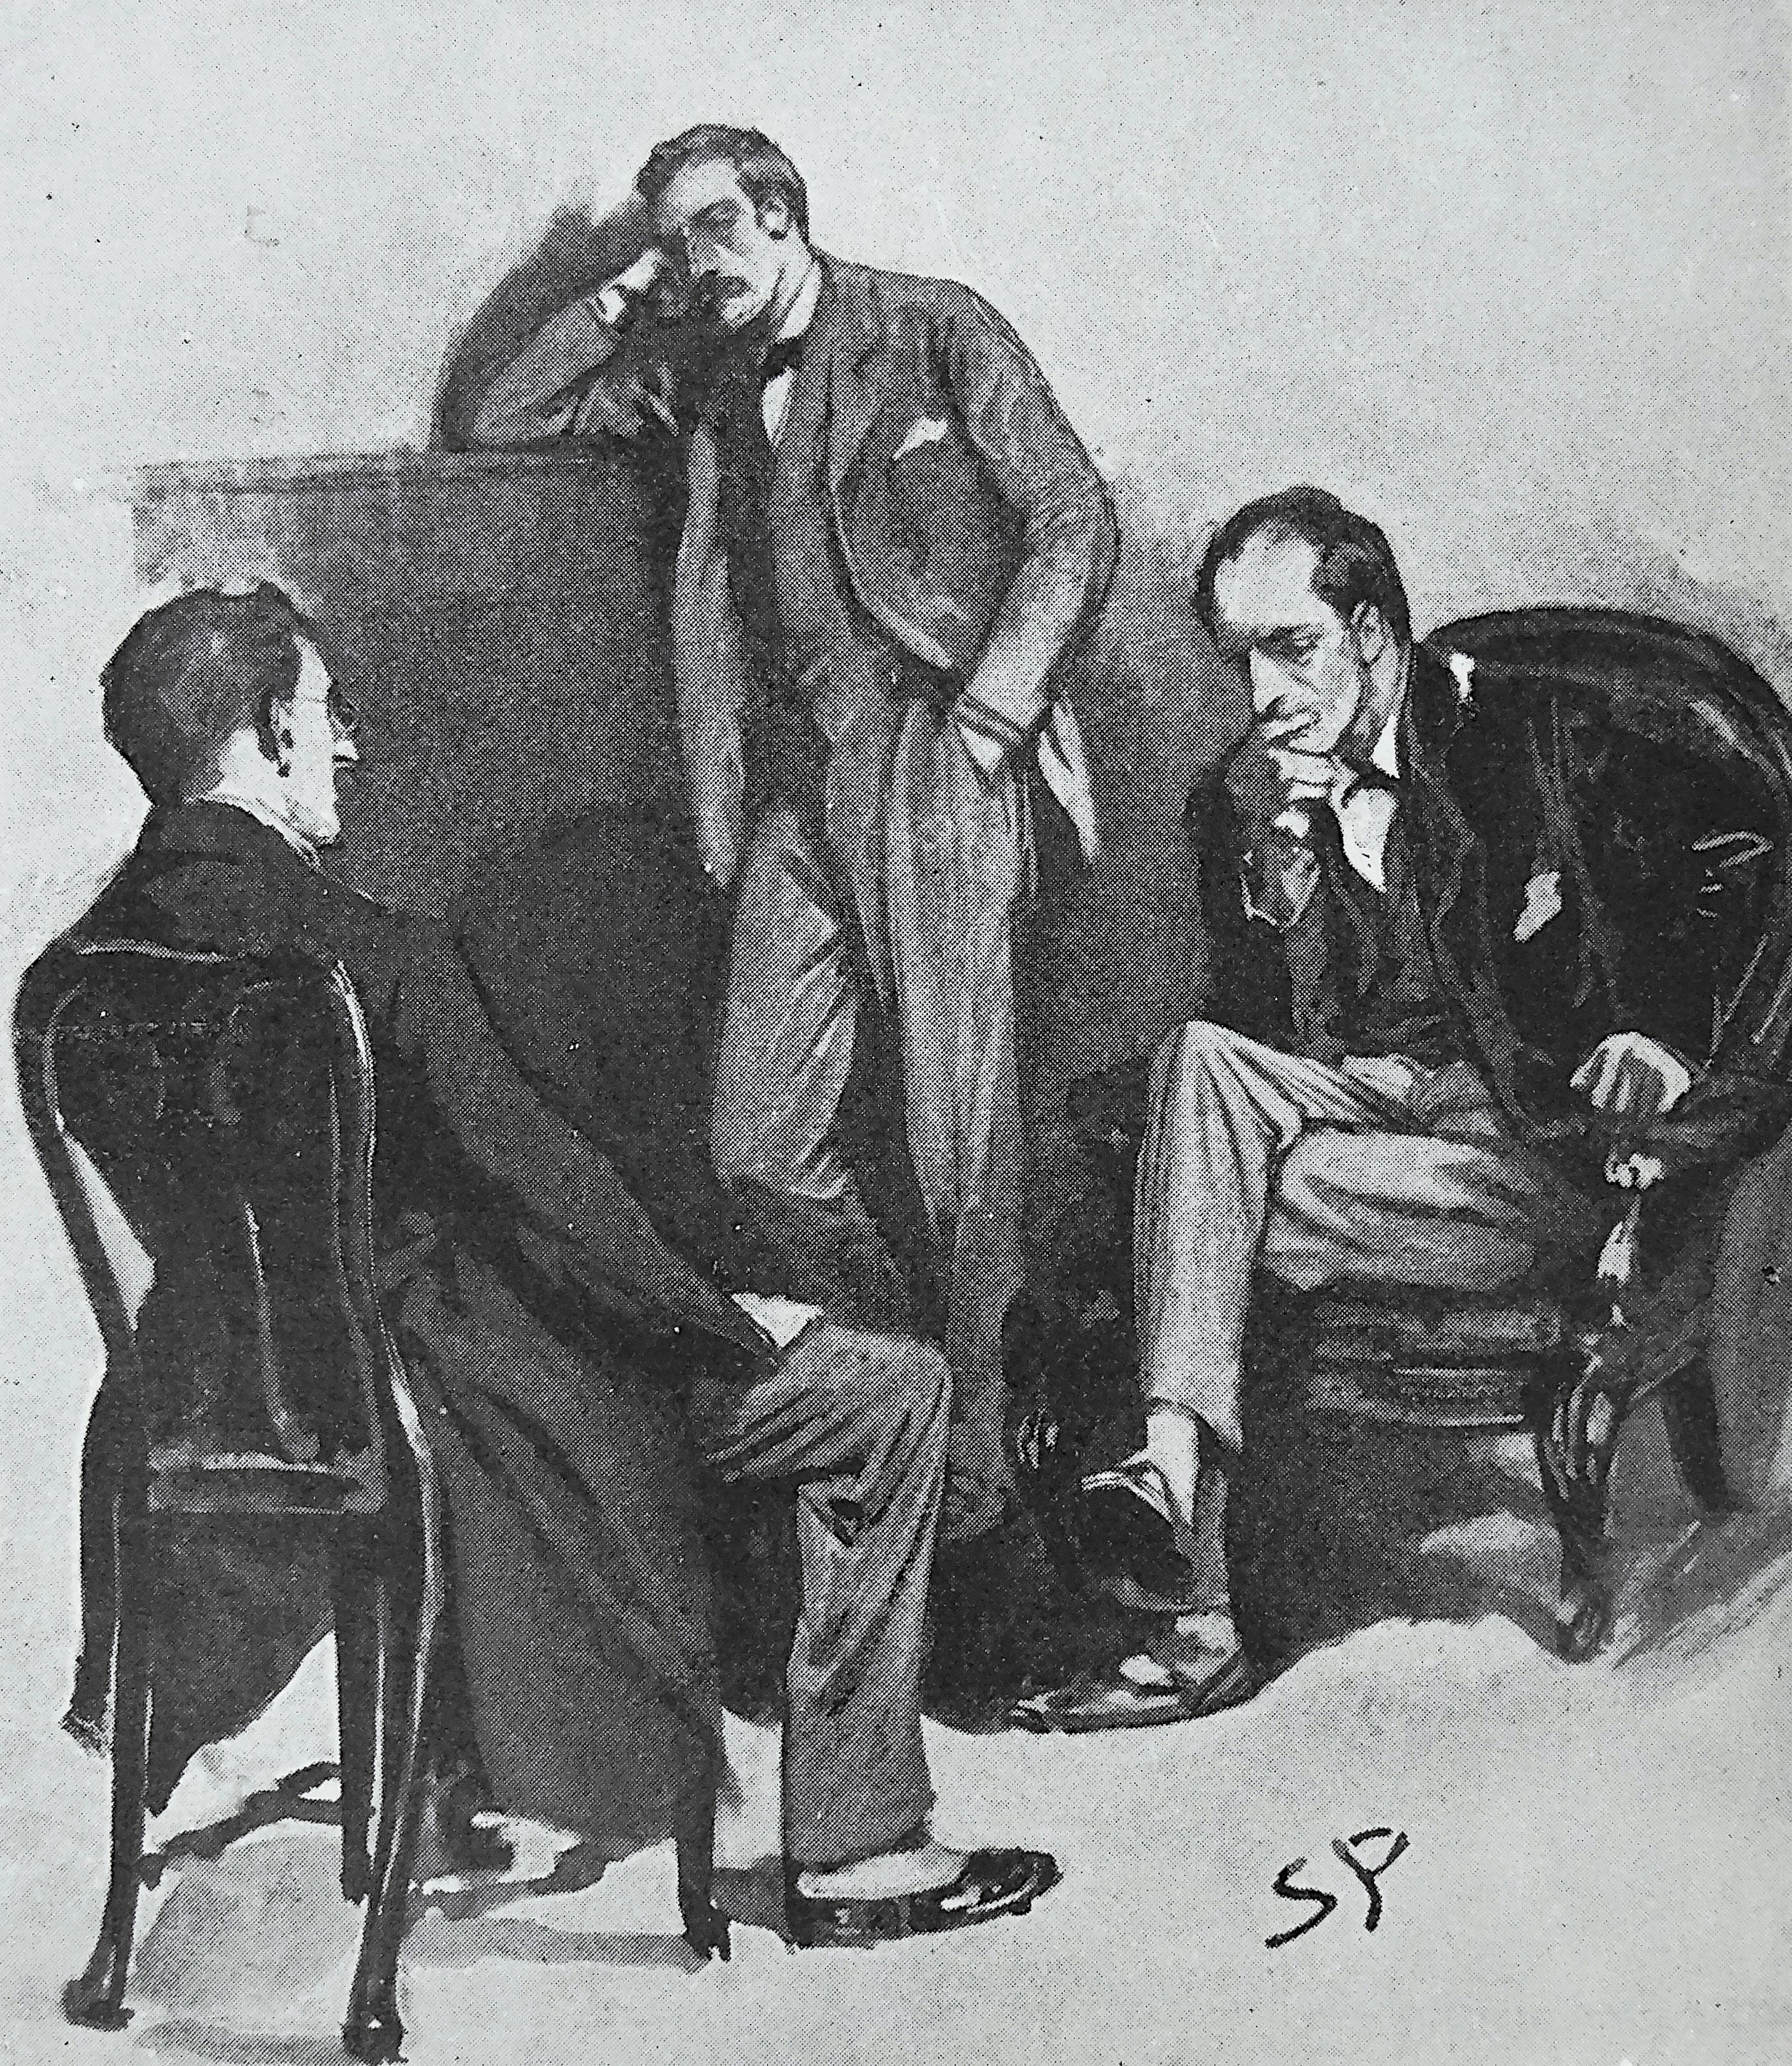
\includegraphics[width=\linewidth]{answerfor}
%\caption{You have indeed much to answer for}
%\end{figure}
%
%\afterpage{\clearpage}

\enquote{I could not call you in, Mr Holmes, without disclosing these facts to the world, and I have already given my reasons for not wishing to do so. Besides, besides---}

\enquote{Why do you hesitate?}

\enquote{There is a realm in which the most acute and most experienced of detectives is helpless.}

\enquote{You mean that the thing is supernatural?}

\enquote{I did not positively say so.}

\enquote{No, but you evidently think it.}

\enquote{Since the tragedy, Mr Holmes, there have come to my ears several incidents which are hard to reconcile with the settled order of Nature.}

\enquote{For example?}

\enquote{I find that before the terrible event occurred several people had seen a creature upon the moor which corresponds with this Baskerville demon, and which could not possibly be any animal known to science. They all agreed that it was a huge creature, luminous, ghastly, and spectral. I have cross-examined these men, one of them a hard-headed countryman, one a farrier, and one a moorland farmer, who all tell the same story of this dreadful apparition, exactly corresponding to the hell-hound of the legend. I assure you that there is a reign of terror in the district, and that it is a hardy man who will cross the moor at night.}

\enquote{And you, a trained man of science, believe it to be supernatural?}

\enquote{I do not know what to believe.}

Holmes shrugged his shoulders.

\enquote{I have hitherto confined my investigations to this world,} said he. \enquote{In a modest way I have combated evil, but to take on the Father of Evil himself would, perhaps, be too ambitious a task. Yet you must admit that the footmark is material.}

\enquote{The original hound was material enough to tug a man's throat out, and yet he was diabolical as well.}

\enquote{I see that you have quite gone over to the supernaturalists. But now, Dr Mortimer, tell me this. If you hold these views, why have you come to consult me at all? You tell me in the same breath that it is useless to investigate Sir Charles's death, and that you desire me to do it.}

\enquote{I did not say that I desired you to do it.}

\enquote{Then, how can I assist you?}

\enquote{By advising me as to what I should do with Sir Henry Baskerville, who arrives at Waterloo Station}---Dr Mortimer looked at his watch--- \enquote{in exactly one hour and a quarter.}

\enquote{He being the heir?}

\enquote{Yes. On the death of Sir Charles we inquired for this young gentleman and found that he had been farming in Canada. From the accounts which have reached us he is an excellent fellow in every way. I speak not as a medical man but as a trustee and executor of Sir Charles's will.}

\enquote{There is no other claimant, I presume?}

\enquote{None. The only other kinsman whom we have been able to trace was Rodger Baskerville, the youngest of three brothers of whom poor Sir Charles was the elder. The second brother, who died young, is the father of this lad Henry. The third, Rodger, was the black sheep of the family. He came of the old masterful Baskerville strain, and was the very image, they tell me, of the family picture of old Hugo. He made England too hot to hold him, fled to Central America, and died there in 1876 of yellow fever. Henry is the last of the Baskervilles. In one hour and five minutes I meet him at Waterloo Station. I have had a wire that he arrived at Southampton this morning. Now, Mr Holmes, what would you advise me to do with him?}

\enquote{Why should he not go to the home of his fathers?}

\enquote{It seems natural, does it not? And yet, consider that every Baskerville who goes there meets with an evil fate. I feel sure that if Sir Charles could have spoken with me before his death he would have warned me against bringing this, the last of the old race, and the heir to great wealth, to that deadly place. And yet it cannot be denied that the prosperity of the whole poor, bleak country-side depends upon his presence. All the good work which has been done by Sir Charles will crash to the ground if there is no tenant of the Hall. I fear lest I should be swayed too much by my own obvious interest in the matter, and that is why I bring the case before you and ask for your advice.}

Holmes considered for a little time.

\enquote{Put into plain words, the matter is this,} said he. \enquote{In your opinion there is a diabolical agency which makes Dartmoor an unsafe abode for a Baskerville---that is your opinion?}

\enquote{At least I might go the length of saying that there is some evidence that this may be so.}

\enquote{Exactly. But surely, if your supernatural theory be correct, it could work the young man evil in London as easily as in Devonshire. A devil with merely local powers like a parish vestry would be too inconceivable a thing.}

\enquote{You put the matter more flippantly, Mr Holmes, than you would probably do if you were brought into personal contact with these things. Your advice, then, as I understand it, is that the young man will be as safe in Devonshire as in London. He comes in fifty minutes. What would you recommend?}

\enquote{I recommend, sir, that you take a cab, call off your spaniel who is scratching at my front door, and proceed to Waterloo to meet Sir Henry Baskerville.}

\enquote{And then?}

\enquote{And then you will say nothing to him at all until I have made up my mind about the matter.}

\enquote{How long will it take you to make up your mind?}

\enquote{Twenty-four hours. At ten o'clock to-morrow, Dr Mortimer, I will be much obliged to you if you will call upon me here, and it will be of help to me in my plans for the future if you will bring Sir Henry Baskerville with you.}

\enquote{I will do so, Mr Holmes.} He scribbled the appointment on his shirtcuff and hurried off in his strange, peering, absent-minded fashion. Holmes stopped him at the head of the stair.
%
%\begin{figure}[tbhp]
%\centering
%\includegraphics[width=0.7\linewidth]{03_shirtcuff}
%\caption*{He scribbled the appointment on his shirtcuff}
%\end{figure}

\enquote{Only one more question, Dr Mortimer. You say that before Sir Charles Baskerville's death several people saw this apparition upon the moor?}

\enquote{Three people did.}

\enquote{Did any see it after?}

\enquote{I have not heard of any.}

\enquote{Thank you. Good morning.}

Holmes returned to his seat with that quiet look of inward satisfaction which meant that he had a congenial task before him.

\enquote{Going out, Watson?}

\enquote{Unless I can help you.}

\enquote{No, my dear fellow, it is at the hour of action that I turn to you for aid. But this is splendid, really unique from some points of view. When you pass Bradley's, would you ask him to send up a pound of the strongest shag tobacco? Thank you. It would be as well if you could make it convenient not to return before evening. Then I should be very glad to compare impressions as to this most interesting problem which has been submitted to us this morning.}

I knew that seclusion and solitude were very necessary for my friend in those hours of intense mental concentration during which he weighed every particle of evidence, constructed alternative theories, balanced one against the other, and made up his mind as to which points were essential and which immaterial. I therefore spent the day at my club and did not return to Baker Street until evening. It was nearly nine o'clock when I found myself in the sitting-room once more.

My first impression as I opened the door was that a fire had broken out, for the room was so filled with smoke that the light of the lamp upon the table was blurred by it. As I entered, however, my fears were set at rest, for it was the acrid fumes of strong coarse tobacco which took me by the throat and set me coughing. Through the haze I had a vague vision of Holmes in his dressing-gown coiled up in an armchair with his black clay pipe between his lips. Several rolls of paper lay around him.

\enquote{Caught cold, Watson?} said he.

\enquote{No, it's this poisonous atmosphere.}

\enquote{I suppose it \emph{is} pretty thick, now that you mention it.}

\enquote{Thick! It is intolerable.}

\enquote{Open the window, then! You have been at your club all day, I perceive.}

\enquote{My dear Holmes!}

\enquote{Am I right?}

\enquote{Certainly, but how?}

He laughed at my bewildered expression.

\enquote{There is a delightful freshness about you, Watson, which makes it a pleasure to exercise any small powers which I possess at your expense. A gentleman goes forth on a showery and miry day. He returns immaculate in the evening with the gloss still on his hat and his boots. He has been a fixture therefore all day. He is not a man with intimate friends. Where, then, could he have been? Is it not obvious?}

\enquote{Well, it is rather obvious.}

\enquote{The world is full of obvious things which nobody by any chance ever observes. Where do you think that I have been?}

\enquote{A fixture also.}

\enquote{On the contrary, I have been to Devonshire.}

\enquote{In spirit?}

\enquote{Exactly. My body has remained in this arm-chair and has, I regret to observe, consumed in my absence two large pots of coffee and an incredible amount of tobacco. After you left I sent down to Stamford's for the Ordnance map of this portion of the moor, and my spirit has hovered over it all day. I flatter myself that I could find my way about.}

\enquote{A large scale map, I presume?}

\enquote{Very large.} He unrolled one section and held it over his knee. \enquote{Here you have the particular district which concerns us. That is Baskerville Hall in the middle.}

\enquote{With a wood round it?}

\begin{figure}[tbhp]
\centering
\includegraphics[width=.8\linewidth]{03_baskerhall}
\caption{That is Baskerville Hall in the middle.}
\end{figure}

\enquote{Exactly. I fancy the Yew Alley, though not marked under that name, must stretch along this line, with the moor, as you perceive, upon the right of it. This small clump of buildings here is the hamlet of Grimpen, where our friend Dr Mortimer has his headquarters. Within a radius of five miles there are, as you see, only a very few scattered dwellings. Here is Lafter Hall, which was mentioned in the narrative. There is a house indicated here which may be the residence of the naturalist---Stapleton, if I remember right, was his name. Here are two moorland farm-houses, High Tor and Foulmire. Then fourteen miles away the great convict prison of Princetown. Between and around these scattered points extends the desolate, lifeless moor. This, then, is the stage upon which tragedy has been played, and upon which we may help to play it again.}

\enquote{It must be a wild place.}

\enquote{Yes, the setting is a worthy one. If the devil did desire to have a hand in the affairs of men---}

\enquote{Then you are yourself inclining to the supernatural explanation.}

\enquote{The devil's agents may be of flesh and blood, may they not? There are two questions waiting for us at the outset. The one is whether any crime has been committed at all; the second is, what is the crime and how was it committed? Of course, if Dr Mortimer's surmise should be correct, and we are dealing with forces outside the ordinary laws of Nature, there is an end of our investigation. But we are bound to exhaust all other hypotheses before falling back upon this one. I think we'll shut that window again, if you don't mind. It is a singular thing, but I find that a concentrated atmosphere helps a concentration of thought. I have not pushed it to the length of getting into a box to think, but that is the logical outcome of my convictions. Have you turned the case over in your mind?}

\enquote{Yes, I have thought a good deal of it in the course of the day.}

\enquote{What do you make of it?}

\enquote{It is very bewildering.}

\enquote{It has certainly a character of its own. There are points of distinction about it. That change in the footprints, for example. What do you make of that?}

\enquote{Mortimer said that the man had walked on tiptoe down that portion of the alley.}

\enquote{He only repeated what some fool had said at the inquest. Why should a man walk on tiptoe down the alley?}

\enquote{What then?}

\enquote{He was running, Watson---running desperately, running for his life, running until he burst his heart and fell dead upon his face.}

\enquote{Running from what?}

\enquote{There lies our problem. There are indications that the man was crazed with fear before ever he began to run.}

\enquote{How can you say that?}

\enquote{I am presuming that the cause of his fears came to him across the moor. If that were so, and it seems most probable, only a man who had lost his wits would have run \emph{from} the house instead of towards it. If the gipsy's evidence may be taken as true, he ran with cries for help in the direction where help was least likely to be. Then, again, whom was he waiting for that night, and why was he waiting for him in the Yew Alley rather than in his own house?}

\enquote{You think that he was waiting for someone?}

\enquote{The man was elderly and infirm. We can understand his taking an evening stroll, but the ground was damp and the night inclement. Is it natural that he should stand for five or ten minutes, as Dr Mortimer, with more practical sense than I should have given him credit for, deduced from the cigar ash?}

\enquote{But he went out every evening.}

\enquote{I think it unlikely that he waited at the moor-gate every evening. On the contrary, the evidence is that he avoided the moor. That night he waited there. It was the night before he made his departure for London. The thing takes shape, Watson. It becomes coherent. Might I ask you to hand me my violin, and we will postpone all further thought upon this business until we have had the advantage of meeting Dr Mortimer and Sir Henry Baskerville in the morning.}
\clearpage
\vfill
\begin{figure}[ph!]
\centering
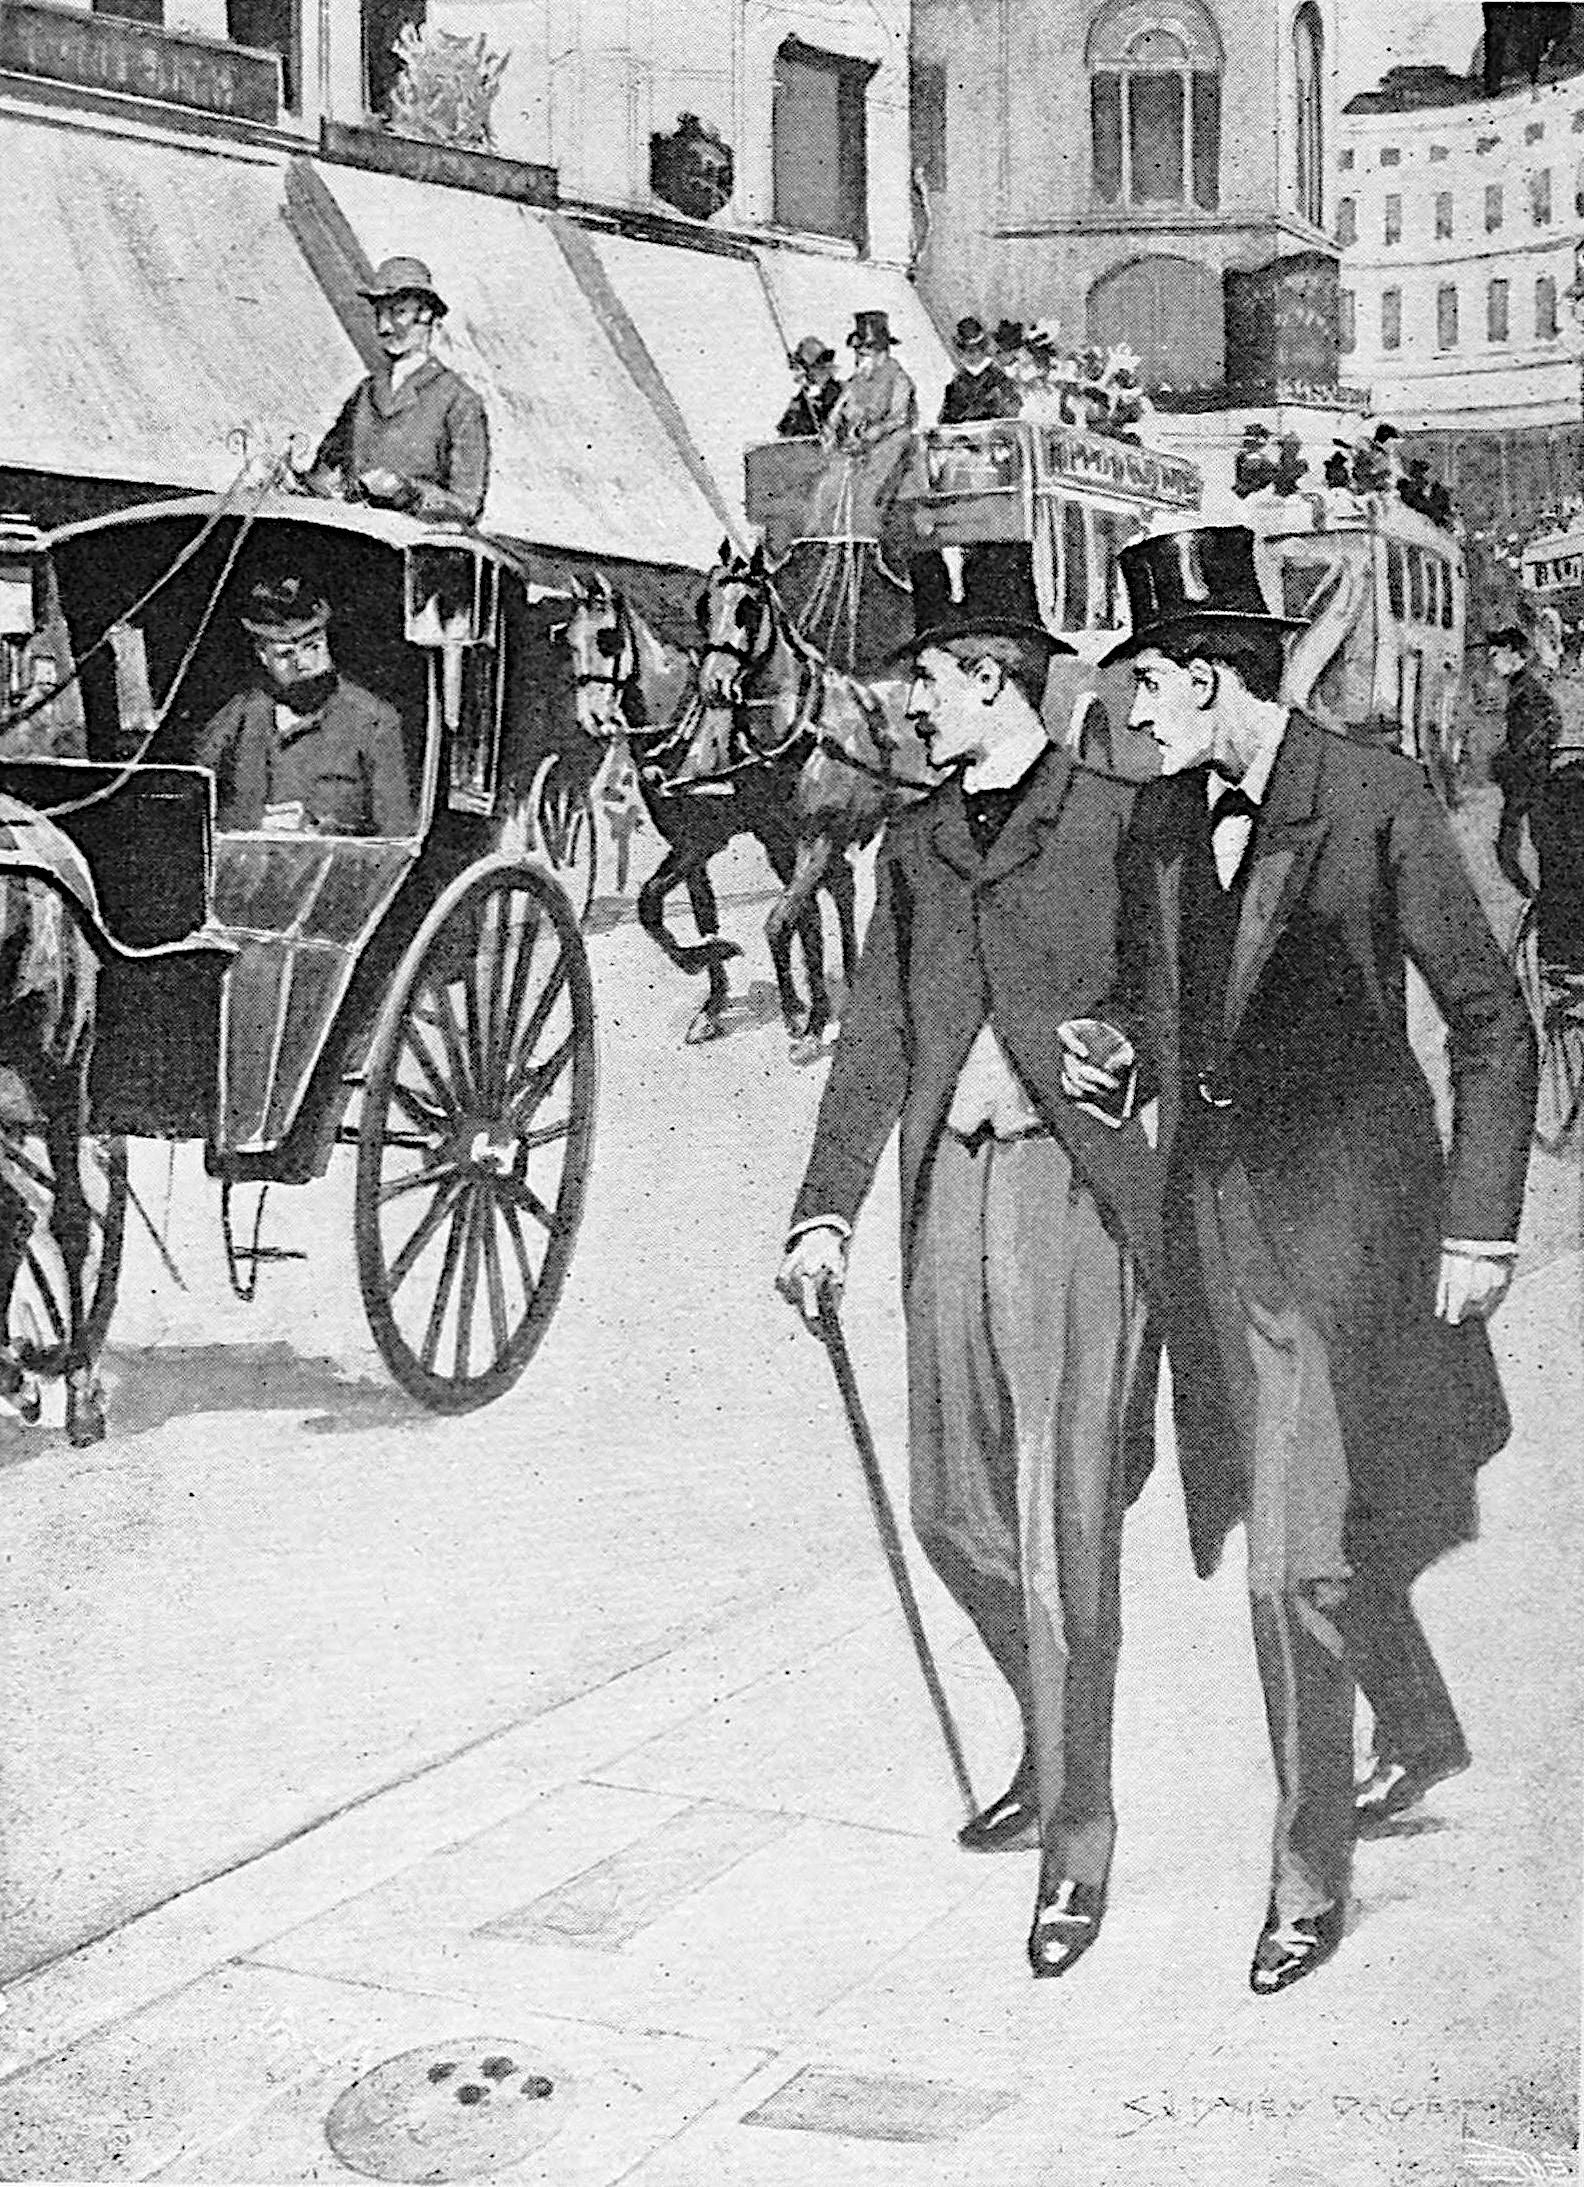
\includegraphics[width=\linewidth]{04_ourman}
\caption{There's our man, Watson!}
\end{figure}
\vfill
\thispagestyle{empty}
\clearpage


%!TeX root=../houndtop.tex
\chapter{Sir Henry Baskerville}
\lettrine[lines=1]{O}{ur} breakfast-table was cleared early, and Holmes waited in his dressing-gown for the promised interview. Our clients were punctual to their appointment, for the clock had just struck ten when Dr Mortimer was shown up, followed by the young baronet. The latter was a small, alert, dark-eyed man about thirty years of age, very sturdily built, with thick black eyebrows and a strong, pugnacious face. He wore a ruddy-tinted tweed suit and had the weather-beaten appearance of one who has spent most of his time in the open air, and yet there was something in his steady eye and the quiet assurance of his bearing which indicated the gentleman.

\enquote{This is Sir Henry Baskerville,} said Dr Mortimer.

%\begin{figure}[tbph]
%\centering
%\includegraphics[width=.9\linewidth]{04_sirhenry}
%\caption{Sir Henry Baskerville}
%\end{figure}

\enquote{Why, yes,} said he, \enquote{and the strange thing is, Mr Sherlock Holmes, that if my friend here had not proposed coming round to you this morning I should have come on my own account. I understand that you think out little puzzles, and I've had one this morning which wants more thinking out than I am able to give it.}

\enquote{Pray take a seat, Sir Henry. Do I understand you to say that you have yourself had some remarkable experience since you arrived in London?}

\enquote{Nothing of much importance, Mr Holmes. Only a joke, as like as not. It was this letter, if you can call it a letter, which reached me this morning.}

He laid an envelope upon the table, and we all bent over it. It was of common quality, grayish in colour. The address, \enquote{Sir Henry Baskerville, Northumberland Hotel,} was printed in rough characters; the postmark \enquote{Charing Cross,} and the date of posting the preceding evening.

\enquote{Who knew that you were going to the Northumberland Hotel?} asked Holmes, glancing keenly across at our visitor.

\enquote{No one could have known. We only decided after I met Dr Mortimer.}

\enquote{But Dr Mortimer was no doubt already stopping there?}

\enquote{No, I had been staying with a friend,} said the doctor. \enquote{There was no possible indication that we intended to go to this hotel.}

\enquote{Hum! Someone seems to be very deeply interested in your movements.} Out of the envelope he took a half-sheet of foolscap paper folded into four. This he opened and spread flat upon the table. Across the middle of it a single sentence had been formed by the expedient of pasting printed words upon it. It ran: \enquote{As you value your life or your reason keep away from the moor.} The word \enquote{moor} only was printed in ink.

\enquote{Now,} said Sir Henry Baskerville, \enquote{perhaps you will tell me, Mr Holmes, what in thunder is the meaning of that, and who it is that takes so much interest in my affairs?}

\enquote{What do you make of it, Dr Mortimer? You must allow that there is nothing supernatural about this, at any rate?}

\enquote{No, sir, but it might very well come from someone who was convinced that the business is supernatural.}

\enquote{What business?} asked Sir Henry sharply. \enquote{It seems to me that all you gentlemen know a great deal more than I do about my own affairs.}

\enquote{You shall share our knowledge before you leave this room, Sir Henry. I promise you that,} said Sherlock Holmes. \enquote{We will confine ourselves for the present with your permission to this very interesting document, which must have been put together and posted yesterday evening. Have you yesterday's \textit{Times}, Watson?}

\enquote{It is here in the corner.}

\enquote{Might I trouble you for it---the inside page, please, with the leading articles?}  He glanced swiftly over it, running his eyes up and down the columns. \enquote{Capital article this on free trade. Permit me to give you an extract from it. \enquote{You may be cajoled into imagining that your own special trade or your own industry will be encouraged by a protective tariff, but it stands to reason that such legislation must in the long run keep away wealth from the country, diminish the value of our imports, and lower the general conditions of life in this island.} What do you think of that, Watson?} cried Holmes in high glee, rubbing his hands together with satisfaction. \enquote{Don't you think that is an admirable sentiment?}


Dr Mortimer looked at Holmes with an air of professional interest, and Sir Henry Baskerville turned a pair of puzzled dark eyes upon me.

\enquote{I don't know much about the tariff and things of that kind,} said he; \enquote{but it seems to me we've got a bit off the trail so far as that note is concerned.}

%\begin{figure}[tbhp]
%\centering
%\includegraphics[width=0.8\linewidth]{04_glanced}
%\caption{He glanced swiftly over it}
%\end{figure}


\enquote{On the contrary, I think we are particularly hot upon the trail, Sir Henry. Watson here knows more about my methods than you do, but I fear that even he has not quite grasped the significance of this sentence.}

\enquote{No, I confess that I see no connection.}

\enquote{And yet, my dear Watson, there is so very close a connection that the one is extracted out of the other. \enquote{You}, \enquote{your}, \enquote{your}, \enquote{life}, \enquote{reason}, \enquote{value}, \enquote{keep away}, \enquote{from the}. Don't you see now whence these words have been taken?}

\enquote{By thunder, you're right! Well, if that isn't smart!} cried Sir Henry.

\enquote{If any possible doubt remained it is settled by the fact that \enquote{keep away} and \enquote{from the} are cut out in one piece.}

\enquote{Well, now---so it is!}

\enquote{Really, Mr Holmes, this exceeds anything which I could have imagined,} said Dr Mortimer, gazing at my friend in amazement. \enquote{I could understand anyone saying that the words were from a newspaper; but that you should name which, and add that it came from the leading article, is really one of the most remarkable things which I have ever known. How did you do it?}

\enquote{I presume, Doctor, that you could tell the skull of a negro from that of an Esquimau?\footnote{The Inuit people of the circumpolar region.}}

\enquote{Most certainly.}

\enquote{But how?}

\enquote{Because that is my special hobby. The differences are obvious. The supra-orbital crest, the facial angle, the maxillary curve, \newline the---}

\enquote{But this is my special hobby, and the differences are equally obvious. There is as much difference to my eyes between the leaded bourgeois type of a \textit{Times} article and the slovenly print of an evening half-penny paper as there could be between your negro and your Esquimau. The detection of types is one of the most elementary branches of knowledge to the special expert in crime, though I confess that once when I was very young I confused the \textit{Leeds Mercury} with the \textit{Western Morning News}. But a \textit{Times} leader is entirely distinctive, and these words could have been taken from nothing else. As it was done yesterday the strong probability was that we should find the words in yesterday's issue.}

\enquote{So far as I can follow you, then, Mr Holmes,} said Sir Henry Baskerville, \enquote{someone cut out this message with a scissors---}

\enquote{Nail-scissors,} said Holmes. \enquote{You can see that it was a very short-bladed scissors, since the cutter had to take two snips over \enquote{keep away.}}

\enquote{That is so. Someone, then, cut out the message with a pair of short-bladed scissors, pasted it with paste---}

\enquote{Gum,} said Holmes.

\enquote{With gum on to the paper. But I want to know why the word \enquote{moor} should have been written?}

\enquote{Because he could not find it in print. The other words were all simple and might be found in any issue, but \enquote{moor} would be less common.}

\enquote{Why, of course, that would explain it. Have you read anything else in this message, Mr Holmes?}

%\begin{wrapfigure}{O}{0.5\linewidth}
%\centering
%\includegraphics[width=.5\linewidth]{04_inch}
%\caption*{Holding it only an inch or two from his eyes}
%\end{wrapfigure}

\begin{figure}[tbhp]
\centering
\includegraphics[width=.7\linewidth]{04_inchdetail}
\caption{Holding it only an inch or two from his eyes}
\end{figure}

\enquote{There are one or two indications, and yet the utmost pains have been taken to remove all clues. The address, you observe is printed in rough characters. But the \textit{Times} is a paper which is seldom found in any hands but those of the highly educated. We may take it, therefore, that the letter was composed by an educated man who wished to pose as an uneducated one, and his effort to conceal his own writing suggests that that writing might be known, or come to be known, by you. Again, you will observe that the words are not gummed on in an accurate line, but that some are much higher than others. \enquote{Life}, for example is quite out of its proper place. That may point to carelessness or it may point to agitation and hurry upon the part of the cutter. On the whole I incline to the latter view, since the matter was evidently important, and it is unlikely that the composer of such a letter would be careless. If he were in a hurry it opens up the interesting question why he should be in a hurry, since any letter posted up to early morning would reach Sir Henry before he would leave his hotel. Did the composer fear an interruption---and from whom?}

\enquote{We are coming now rather into the region of guesswork,} said Dr Mortimer.

\enquote{Say, rather, into the region where we balance probabilities and choose the most likely. It is the scientific use of the imagination, but we have always some material basis on which to start our speculation. Now, you would call it a guess, no doubt, but I am almost certain that this address has been written in a hotel.}

\enquote{How in the world can you say that?}

\enquote{If you examine it carefully you will see that both the pen and the ink have given the writer trouble. The pen has spluttered twice in a single word, and has run dry three times in a short address, showing that there was very little ink in the bottle. Now, a private pen or ink-bottle is seldom allowed to be in such a state, and the combination of the two must be quite rare. But you know the hotel ink and the hotel pen, where it is rare to get anything else. Yes, I have very little hesitation in saying that could we examine the waste-paper baskets of the hotels around Charing Cross until we found the remains of the mutilated \textit{Times} leader we could lay our hands straight upon the person who sent this singular message. Halloa! Halloa! What's this?}

He was carefully examining the foolscap, upon which the words were pasted, holding it only an inch or two from his eyes.

\enquote{Well?}

\enquote{Nothing,} said he, throwing it down. \enquote{It is a blank half-sheet of paper, without even a water-mark upon it. I think we have drawn as much as we can from this curious letter; and now, Sir Henry, has anything else of interest happened to you since you have been in London?}

\enquote{Why, no, Mr Holmes. I think not.}

\enquote{You have not observed anyone follow or watch you?}

\enquote{I seem to have walked right into the thick of a dime novel,} said our visitor. \enquote{Why in thunder should anyone follow or watch me?}

\enquote{We are coming to that. You have nothing else to report to us before we go into this matter?}

\enquote{Well, it depends upon what you think worth reporting.}

\enquote{I think anything out of the ordinary routine of life well worth reporting.}

Sir Henry smiled.

\enquote{I don't know much of British life yet, for I have spent nearly all my time in the States and in Canada. But I hope that to lose one of your boots is not part of the ordinary routine of life over here.}

\enquote{You have lost one of your boots?}

\enquote{My dear sir,} cried Dr Mortimer, \enquote{it is only mislaid. You will find it when you return to the hotel. What is the use of troubling Mr Holmes with trifles of this kind?}

\enquote{Well, he asked me for anything outside the ordinary routine.}

\enquote{Exactly,} said Holmes, \enquote{however foolish the incident may seem. You have lost one of your boots, you say?}

\enquote{Well, mislaid it, anyhow. I put them both outside my door last night, and there was only one in the morning. I could get no sense out of the chap who cleans them. The worst of it is that I only bought the pair last night in the Strand, and I have never had them on.}

\enquote{If you have never worn them, why did you put them out to be cleaned?}

\enquote{They were tan boots and had never been varnished. That was why I put them out.}

\enquote{Then I understand that on your arrival in London yesterday you went out at once and bought a pair of boots?}

\enquote{I did a good deal of shopping. Dr Mortimer here went round with me. You see, if I am to be squire down there I must dress the part, and it may be that I have got a little careless in my ways out West. Among other things I bought these brown boots---gave six dollars\footnote{Approximately \textdollar 200 USD in 2023.} for them---and had one stolen before ever I had them on my feet.}

\enquote{It seems a singularly useless thing to steal,} said Sherlock Holmes. \enquote{I confess that I share Dr Mortimer's belief that it will not be long before the missing boot is found.}

\enquote{And, now, gentlemen,} said the baronet with decision, \enquote{it seems to me that I have spoken quite enough about the little that I know. It is time that you kept your promise and gave me a full account of what we are all driving at.}

\enquote{Your request is a very reasonable one,} Holmes answered. \enquote{Dr Mortimer, I think you could not do better than to tell your story as you told it to us.}

Thus encouraged, our scientific friend drew his papers from his pocket, and presented the whole case as he had done upon the morning before. Sir Henry Baskerville listened with the deepest attention, and with an occasional exclamation of surprise.

\enquote{Well, I seem to have come into an inheritance with a vengeance,} said he when the long narrative was finished. \enquote{Of course, I've heard of the hound ever since I was in the nursery. It's the pet story of the family, though I never thought of taking it seriously before. But as to my uncle's death---well, it all seems boiling up in my head, and I can't get it clear yet. You don't seem quite to have made up your mind whether it's a case for a policeman or a clergyman.}

\enquote{Precisely.}

\enquote{And now there's this affair of the letter to me at the hotel. I suppose that fits into its place.}

\enquote{It seems to show that someone knows more than we do about what goes on upon the moor,} said Dr Mortimer.

\enquote{And also,} said Holmes, \enquote{that someone is not ill-disposed towards you, since they warn you of danger.}

\enquote{Or it may be that they wish, for their own purposes, to scare me away.}

\enquote{Well, of course, that is possible also. I am very much indebted to you, Dr Mortimer, for introducing me to a problem which presents several interesting alternatives. But the practical point which we now have to decide, Sir Henry, is whether it is or is not advisable for you to go to Baskerville Hall.}

\enquote{Why should I not go?}

\enquote{There seems to be danger.}

\enquote{Do you mean danger from this family fiend or do you mean danger from human beings?}

\enquote{Well, that is what we have to find out.}

\enquote{Whichever it is, my answer is fixed. There is no devil in hell, Mr Holmes, and there is no man upon earth who can prevent me from going to the home of my own people, and you may take that to be my final answer.} His dark brows knitted and his face flushed to a dusky red as he spoke. It was evident that the fiery temper of the Baskervilles was not extinct in this their last representative. \enquote{Meanwhile,} said he, \enquote{I have hardly had time to think over all that you have told me. It's a big thing for a man to have to understand and to decide at one sitting. I should like to have a quiet hour by myself to make up my mind. Now, look here, Mr Holmes, it's half-past eleven now and I am going back right away to my hotel. Suppose you and your friend, Dr Watson, come round and lunch with us at two. I'll be able to tell you more clearly then how this thing strikes me.}

\enquote{Is that convenient to you, Watson?}

\enquote{Perfectly.}

\enquote{Then you may expect us. Shall I have a cab called?}

\enquote{I'd prefer to walk, for this affair has flurried me rather.}

\enquote{I'll join you in a walk, with pleasure,} said his companion.

\enquote{Then we meet again at two o'clock. Au revoir, and good-morning!}

We heard the steps of our visitors descend the stair and the bang of the front door. In an instant Holmes had changed from the languid dreamer to the man of action.

\enquote{Your hat and boots, Watson, quick! Not a moment to lose!} He rushed into his room in his dressing-gown and was back again in a few seconds in a frock-coat. We hurried together down the stairs and into the street. Dr Mortimer and Baskerville were still visible about two hundred yards ahead of us in the direction of Oxford Street.

\enquote{Shall I run on and stop them?}

\enquote{Not for the world, my dear Watson. I am perfectly satisfied with your company if you will tolerate mine. Our friends are wise, for it is certainly a very fine morning for a walk.}

He quickened his pace until we had decreased the distance which divided us by about half. Then, still keeping a hundred yards behind, we followed into Oxford Street and so down Regent Street. Once our friends stopped and stared into a shop window, upon which Holmes did the same. An instant afterwards he gave a little cry of satisfaction, and, following the direction of his eager eyes, I saw that a hansom cab with a man inside which had halted on the other side of the street was now proceeding slowly onward again.

\enquote{There's our man, Watson! Come along! We'll have a good look at him, if we can do no more.}

At that instant I was aware of a bushy black beard and a pair of piercing eyes turned upon us through the side window of the cab. Instantly the trapdoor at the top flew up, something was screamed to the driver, and the cab flew madly off down Regent Street. Holmes looked eagerly round for another, but no empty one was in sight. Then he dashed in wild pursuit amid the stream of the traffic, but the start was too great, and already the cab was out of sight.

\enquote{There now!} said Holmes bitterly as he emerged panting and white with vexation from the tide of vehicles. \enquote{Was ever such bad luck and such bad management, too? Watson, Watson, if you are an honest man you will record this also and set it against my successes!}

\enquote{Who was the man?}

\enquote{I have not an idea.}

\enquote{A spy?}

\enquote{Well, it was evident from what we have heard that Baskerville has been very closely shadowed by someone since he has been in town. How else could it be known so quickly that it was the Northumberland Hotel which he had chosen? If they had followed him the first day I argued that they would follow him also the second. You may have observed that I twice strolled over to the window while Dr Mortimer was reading his legend.}

\enquote{Yes, I remember.}

\enquote{I was looking out for loiterers in the street, but I saw none. We are dealing with a clever man, Watson. This matter cuts very deep, and though I have not finally made up my mind whether it is a benevolent or a malevolent agency which is in touch with us, I am conscious always of power and design. When our friends left I at once followed them in the hopes of marking down their invisible attendant. So wily was he that he had not trusted himself upon foot, but he had availed himself of a cab so that he could loiter behind or dash past them and so escape their notice. His method had the additional advantage that if they were to take a cab he was all ready to follow them. It has, however, one obvious disadvantage.}

\enquote{It puts him in the power of the cabman.}

\enquote{Exactly.}

\enquote{What a pity we did not get the number!}

\enquote{My dear Watson, clumsy as I have been, you surely do not seriously imagine that I neglected to get the number? № 2704 is our man. But that is no use to us for the moment.}

\enquote{I fail to see how you could have done more.}

\enquote{On observing the cab I should have instantly turned and walked in the other direction. I should then at my leisure have hired a second cab and followed the first at a respectful distance, or, better still, have driven to the Northumberland Hotel and waited there. When our unknown had followed Baskerville home we should have had the opportunity of playing his own game upon himself and seeing where he made for. As it is, by an indiscreet eagerness, which was taken advantage of with extraordinary quickness and energy by our opponent, we have betrayed ourselves and lost our man.}

We had been sauntering slowly down Regent Street during this conversation, and Dr Mortimer, with his companion, had long vanished in front of us.

\enquote{There is no object in our following them,} said Holmes. \enquote{The shadow has departed and will not return. We must see what further cards we have in our hands and play them with decision. Could you swear to that man's face within the cab?}

\enquote{I could swear only to the beard.}

\enquote{And so could I---from which I gather that in all probability it was a false one. A clever man upon so delicate an errand has no use for a beard save to conceal his features. Come in here, Watson!}

He turned into one of the district messenger offices, where he was warmly greeted by the manager.

\enquote{Ah, Wilson, I see you have not forgotten the little case in which I had the good fortune to help you?}

\enquote{No, sir, indeed I have not. You saved my good name, and perhaps my life.}

\enquote{My dear fellow, you exaggerate. I have some recollection, Wilson, that you had among your boys a lad named Cartwright, who showed some ability during the investigation.}

\enquote{Yes, sir, he is still with us.}

\enquote{Could you ring him up?---thank you! And I should be glad to have change of this five-pound note.}

A lad of fourteen, with a bright, keen face, had obeyed the summons of the manager. He stood now gazing with great reverence at the famous detective.

\begin{figure}[tbph]
\centering
\includegraphics[width=\linewidth]{05_23hotels}
\caption{Here are the names of twenty-three hotels}
\end{figure}

\enquote{Let me have the Hotel Directory,} said Holmes. \enquote{Thank you! Now, Cartwright, there are the names of twenty-three hotels here, all in the immediate neighbourhood of Charing Cross. Do you see?}

\enquote{Yes, sir.}

\enquote{You will visit each of these in turn.}

\enquote{Yes, sir.}

\enquote{You will begin in each case by giving the outside porter one shilling. Here are twenty-three shillings.}

\enquote{Yes, sir.}

\enquote{You will tell him that you want to see the waste-paper of yesterday. You will say that an important telegram has miscarried and that you are looking for it. You understand?}

\enquote{Yes, sir.}

\enquote{But what you are really looking for is the centre page of the \textit{Times} with some holes cut in it with scissors. Here is a copy of the \textit{Times}. It is this page. You could easily recognize it, could you not?}

\enquote{Yes, sir.}

\enquote{In each case the outside porter will send for the hall porter, to whom also you will give a shilling. Here are twenty-three shillings. You will then learn in possibly twenty cases out of the twenty-three that the waste of the day before has been burned or removed. In the three other cases you will be shown a heap of paper and you will look for this page of the \textit{Times} among it. The odds are enormously against your finding it. There are ten shillings over in case of emergencies. Let me have a report by wire at Baker Street before evening. And now, Watson, it only remains for us to find out by wire the identity of 
the cabman, № 2704, and then we will drop into one of the Bond Street picture galleries and fill in the time until we are due at the hotel.}

%\begin{figure}[p!]
%\centering
%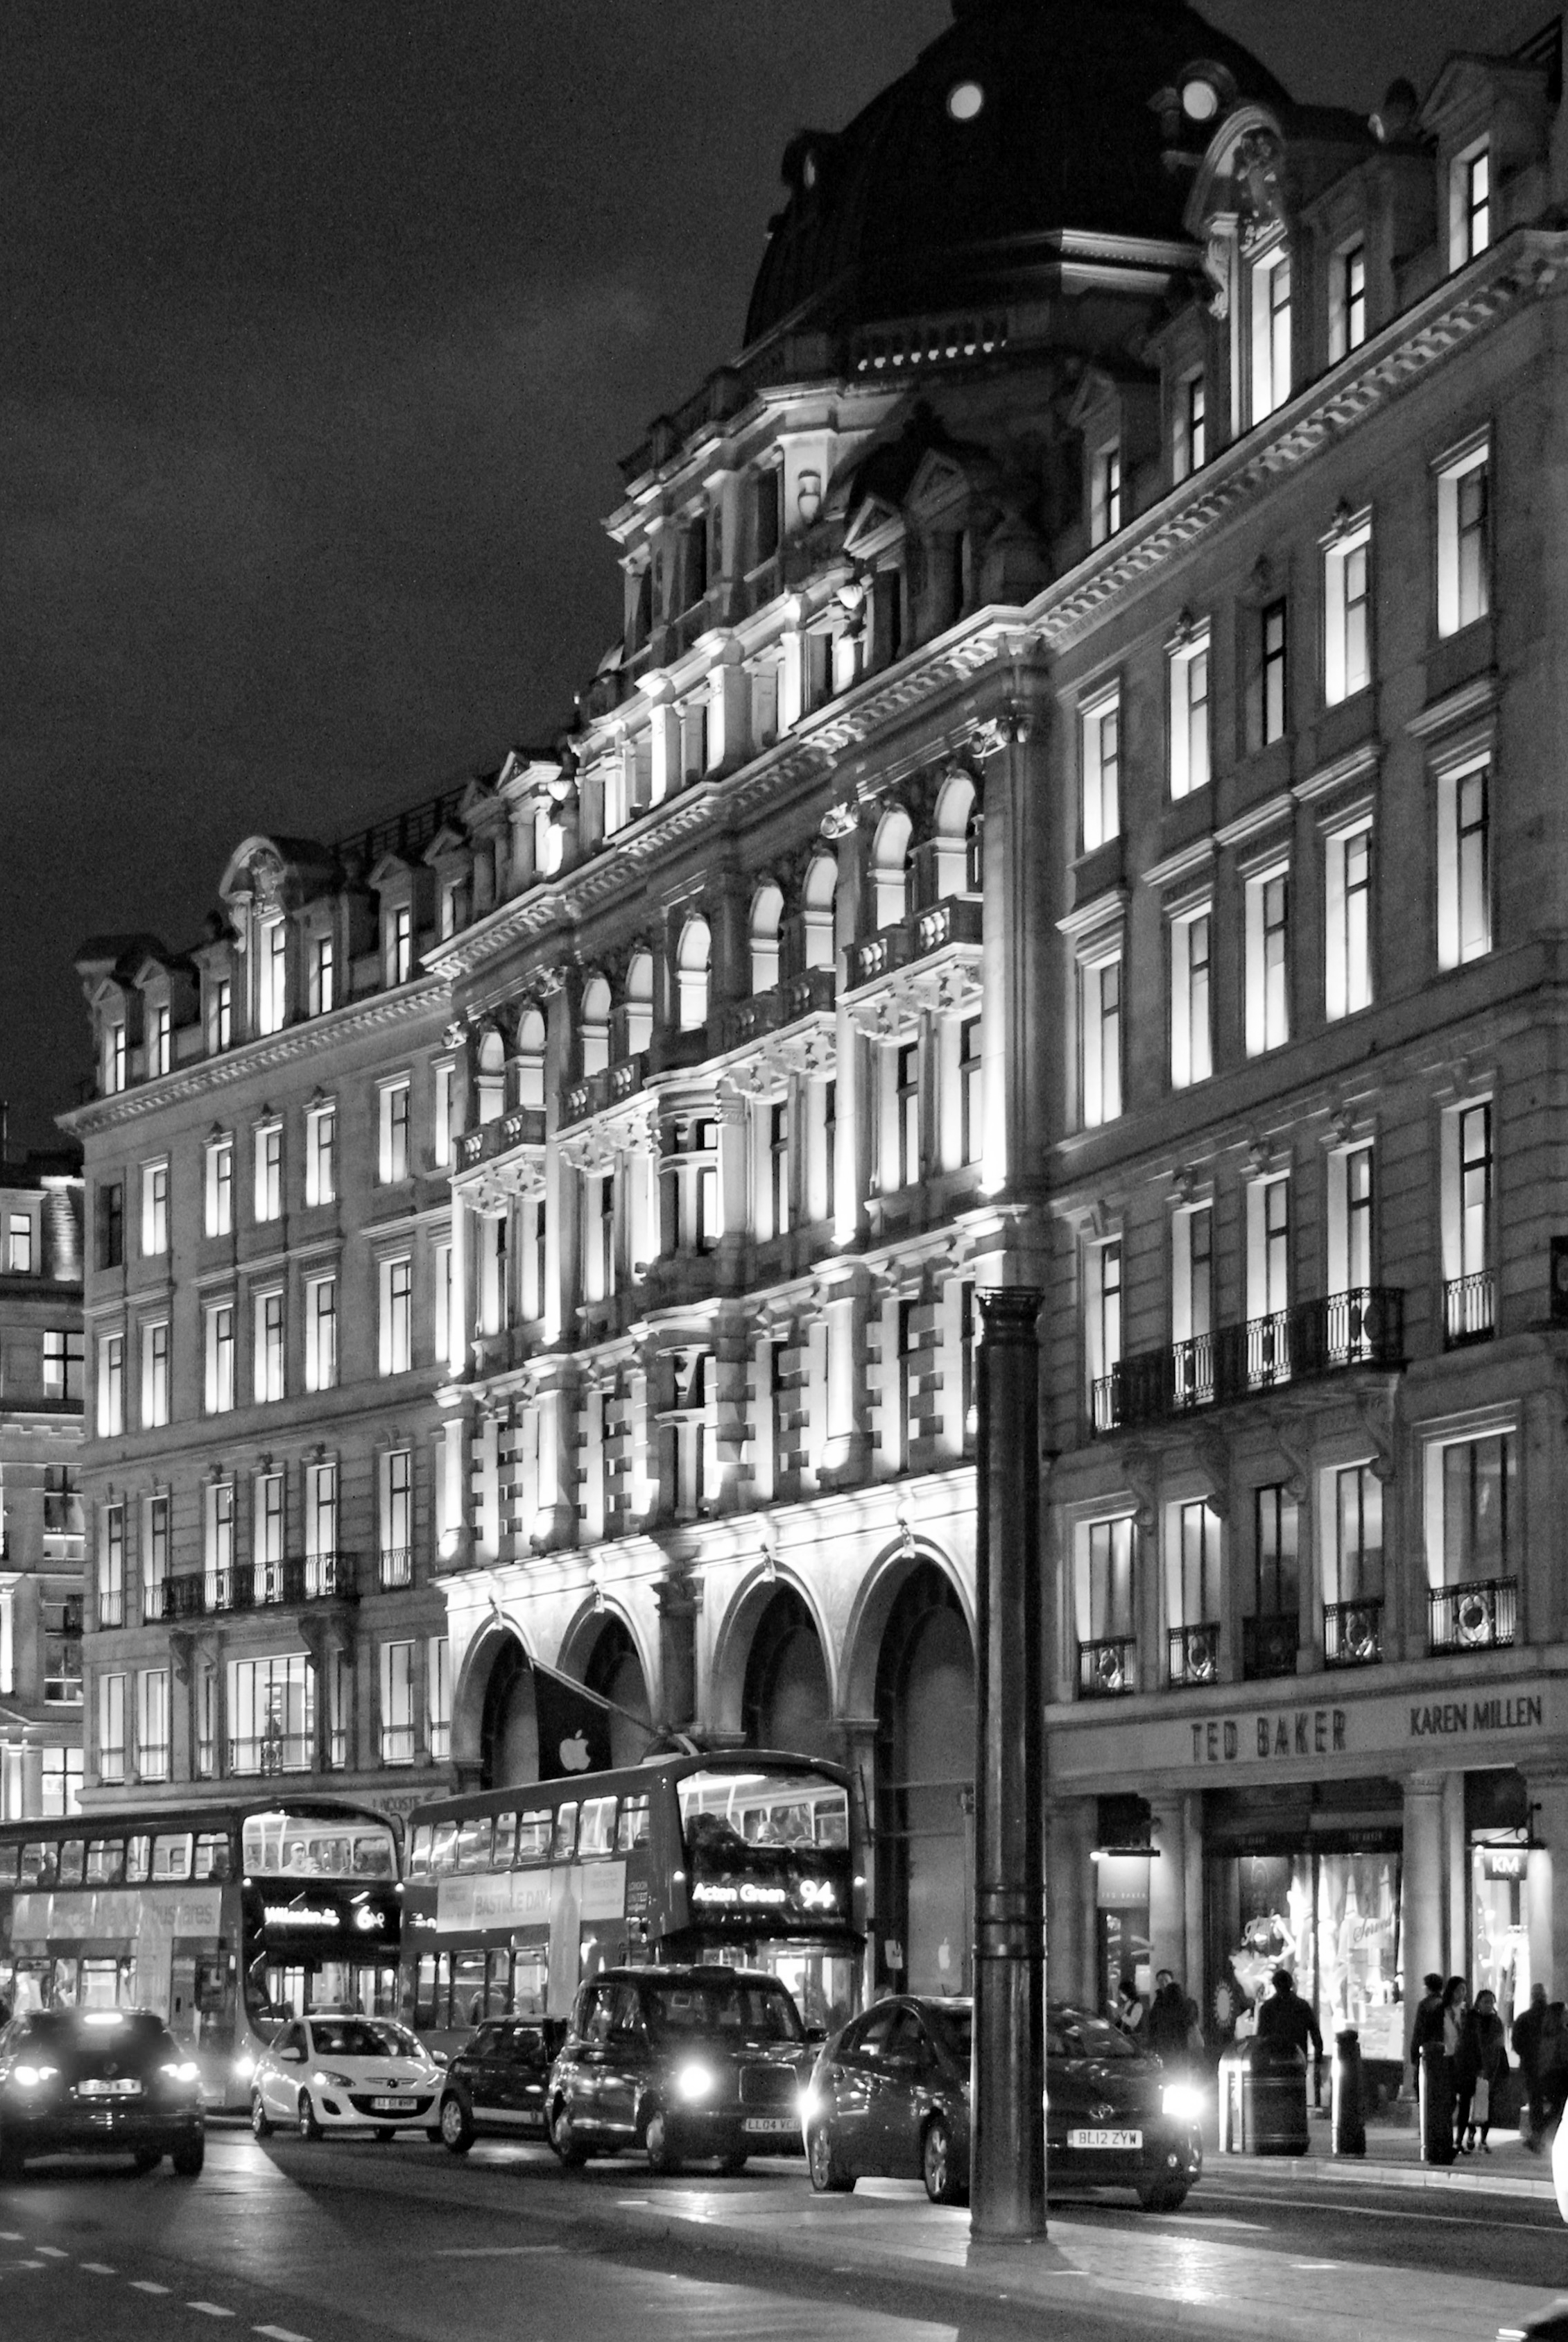
\includegraphics[width=\linewidth]{regentst}
%\caption{\enquote{Busy Regent St At Night}---Can Pac Swire}
%\end{figure}
%\thispagestyle{empty}
%\clearpage
\clearpage
\vfill
\begin{figure}[ph!]
\centering
\includegraphics[width=\linewidth]{05_oldboot}
\caption{He held an old and dusty boot in one of his hands}
\end{figure}
\vfill
\thispagestyle{empty}
\clearpage

%!TeX root=../signtop.tex
\chapter{The Tragedy of Pondicherry Lodge}
\lettrine[lines=4]{I}{t} was nearly eleven o'clock when we reached this final stage of our night's adventures. We had left the damp fog of the great city behind us, and the night was fairly fine. A warm wind blew from the westward, and heavy clouds moved slowly across the sky, with half a moon peeping occasionally through the rifts. It was clear enough to see for some distance, but Thaddeus Sholto took down one of the side-lamps from the carriage to give us a better light upon our way.

Pondicherry Lodge stood in its own grounds, and was girt round with a very high stone wall topped with broken glass. A single narrow iron-clamped door formed the only means of entrance. On this our guide knocked with a peculiar postman-like rat-tat.

»Who is there?« cried a gruff voice from within.

»It is I, McMurdo. You surely know my knock by this time.«

There was a grumbling sound and a clanking and jarring of keys. The door swung heavily back, and a short, deep-chested man stood in the opening, with the yellow light of the lantern shining upon his protruded face and twinkling distrustful eyes.

»That you, Mr Thaddeus? But who are the others? I had no orders about them from the master.«

»No, McMurdo? You surprise me! I told my brother last night that I should bring some friends.«

»He ain't been out o' his room to-day, Mr Thaddeus, and I have no orders. You know very well that I must stick to regulations. I can let you in, but your friends must just stop where they are.«

This was an unexpected obstacle. Thaddeus Sholto looked about him in a perplexed and helpless manner. »This is too bad of you, McMurdo!« he said. »If I guarantee them, that is enough for you. There is the young lady, too. She cannot wait on the public road at this hour.«

»Very sorry, Mr Thaddeus,« said the porter, inexorably. »Folk may be friends o' yours, and yet no friends o' the master's. He pays me well to do my duty, and my duty I'll do. I don't know none o' your friends.«

»Oh, yes you do, McMurdo,« cried Sherlock Holmes, genially. »I don't think you can have forgotten me. Don't you remember the amateur who fought three rounds with you at Alison's rooms on the night of your benefit four years back?«

»Not Mr Sherlock Holmes!« roared the prize-fighter. »God's truth! how could I have mistook you? If instead o' standin' there so quiet you had just stepped up and given me that cross-hit of yours under the jaw, I'd ha' known you without a question. Ah, you're one that has wasted your gifts, you have! You might have aimed high, if you had joined the fancy.«

»You see, Watson, if all else fails me I have still one of the scientific professions open to me,« said Holmes, laughing. »Our friend won't keep us out in the cold now, I am sure.«

»In you come, sir, in you come,—you and your friends,« he answered. »Very sorry, Mr Thaddeus, but orders are very strict. Had to be certain of your friends before I let them in.«

Inside, a gravel path wound through desolate grounds to a huge clump of a house, square and prosaic, all plunged in shadow save where a moonbeam struck one corner and glimmered in a garret window. The vast size of the building, with its gloom and its deathly silence, struck a chill to the heart. Even Thaddeus Sholto seemed ill at ease, and the lantern quivered and rattled in his hand.

»I cannot understand it,« he said. »There must be some mistake. I distinctly told Bartholomew that we should be here, and yet there is no light in his window. I do not know what to make of it.«

»Does he always guard the premises in this way?« asked Holmes.

»Yes; he has followed my father's custom. He was the favourite son, you know, and I sometimes think that my father may have told him more than he ever told me. That is Bartholomew's window up there where the moonshine strikes. It is quite bright, but there is no light from within, I think.«

»None,« said Holmes. »But I see the glint of a light in that little window beside the door.«

»Ah, that is the housekeeper's room. That is where old Mrs Bernstone sits. She can tell us all about it. But perhaps you would not mind waiting here for a minute or two, for if we all go in together and she has no word of our coming she may be alarmed. But hush! what is that?«

He held up the lantern, and his hand shook until the circles of light flickered and wavered all round us. Miss Morstan seized my wrist, and we all stood with thumping hearts, straining our ears. From the great black house there sounded through the silent night the saddest and most pitiful of sounds,—the shrill, broken whimpering of a frightened woman.

»It is Mrs Bernstone,« said Sholto. »She is the only woman in the house. Wait here. I shall be back in a moment.« He hurried for the door, and knocked in his peculiar way. We could see a tall old woman admit him, and sway with pleasure at the very sight of him.

»Oh, Mr Thaddeus, sir, I am so glad you have come! I am so glad you have come, Mr Thaddeus, sir!« We heard her reiterated rejoicings until the door was closed and her voice died away into a muffled monotone.

Our guide had left us the lantern. Holmes swung it slowly round, and peered keenly at the house, and at the great rubbish-heaps which cumbered the grounds. Miss Morstan and I stood together, and her hand was in mine. A wondrous subtle thing is love, for here were we two who had never seen each other before that day, between whom no word or even look of affection had ever passed, and yet now in an hour of trouble our hands instinctively sought for each other. I have marvelled at it since, but at the time it seemed the most natural thing that I should go out to her so, and, as she has often told me, there was in her also the instinct to turn to me for comfort and protection. So we stood hand in hand, like two children, and there was peace in our hearts for all the dark things that surrounded us.

»What a strange place!« she said, looking round.

»It looks as though all the moles in England had been let loose in it. I have seen something of the sort on the side of a hill near Ballarat, where the prospectors had been at work.«

»And from the same cause,« said Holmes. »These are the traces of the treasure-seekers. You must remember that they were six years looking for it. No wonder that the grounds look like a gravel-pit.«

At that moment the door of the house burst open, and Thaddeus Sholto came running out, with his hands thrown forward and terror in his eyes.

»There is something amiss with Bartholomew!« he cried. »I am frightened! My nerves cannot stand it.« He was, indeed, half blubbering with fear, and his twitching feeble face peeping out from the great Astrakhan collar had the helpless appealing expression of a terrified child.

»Come into the house,« said Holmes, in his crisp, firm way.

»Yes, do!« pleaded Thaddeus Sholto. »I really do not feel equal to giving directions.«

We all followed him into the housekeeper's room, which stood upon the left-hand side of the passage. The old woman was pacing up and down with a scared look and restless picking fingers, but the sight of Miss Morstan appeared to have a soothing effect upon her.

»God bless your sweet calm face!« she cried, with an hysterical sob. »It does me good to see you. Oh, but I have been sorely tried this day!«

Our companion patted her thin, work-worn hand, and murmured some few words of kindly womanly comfort which brought the colour back into the other's bloodless cheeks.

»Master has locked himself in and will not answer me,« she explained. »All day I have waited to hear from him, for he often likes to be alone; but an hour ago I feared that something was amiss, so I went up and peeped through the key-hole. You must go up, Mr Thaddeus,—you must go up and look for yourself. I have seen Mr Bartholomew Sholto in joy and in sorrow for ten long years, but I never saw him with such a face on him as that.«

Sherlock Holmes took the lamp and led the way, for Thaddeus Sholto's teeth were chattering in his head. So shaken was he that I had to pass my hand under his arm as we went up the stairs, for his knees were trembling under him. Twice as we ascended Holmes whipped his lens out of his pocket and carefully examined marks which appeared to me to be mere shapeless smudges of dust upon the cocoa-nut matting which served as a stair-carpet. He walked slowly from step to step, holding the lamp, and shooting keen glances to right and left. Miss Morstan had remained behind with the frightened housekeeper.

The third flight of stairs ended in a straight passage of some length, with a great picture in Indian tapestry upon the right of it and three doors upon the left. Holmes advanced along it in the same slow and methodical way, while we kept close at his heels, with our long black shadows streaming backwards down the corridor. The third door was that which we were seeking. Holmes knocked without receiving any answer, and then tried to turn the handle and force it open. It was locked on the inside, however, and by a broad and powerful bolt, as we could see when we set our lamp up against it. The key being turned, however, the hole was not entirely closed. Sherlock Holmes bent down to it, and instantly rose again with a sharp intaking of the breath.

»There is something devilish in this, Watson,« said he, more moved than I had ever before seen him. »What do you make of it?«

I stooped to the hole, and recoiled in horror. Moonlight was streaming into the room, and it was bright with a vague and shifty radiance. Looking straight at me, and suspended, as it were, in the air, for all beneath was in shadow, there hung a face,—the very face of our companion Thaddeus. There was the same high, shining head, the same circular bristle of red hair, the same bloodless countenance. The features were set, however, in a horrible smile, a fixed and unnatural grin, which in that still and moonlit room was more jarring to the nerves than any scowl or contortion. So like was the face to that of our little friend that I looked round at him to make sure that he was indeed with us. Then I recalled to mind that he had mentioned to us that his brother and he were twins.

»This is terrible!« I said to Holmes. »What is to be done?«

»The door must come down,« he answered, and, springing against it, he put all his weight upon the lock. It creaked and groaned, but did not yield. Together we flung ourselves upon it once more, and this time it gave way with a sudden snap, and we found ourselves within Bartholomew Sholto's chamber.

It appeared to have been fitted up as a chemical laboratory. A double line of glass-stoppered bottles was drawn up upon the wall opposite the door, and the table was littered over with Bunsen burners, test-tubes, and retorts. In the corners stood carboys of acid in wicker baskets. One of these appeared to leak or to have been broken, for a stream of dark-coloured liquid had trickled out from it, and the air was heavy with a peculiarly pungent, tar-like odour. A set of steps stood at one side of the room, in the midst of a litter of lath and plaster, and above them there was an opening in the ceiling large enough for a man to pass through. At the foot of the steps a long coil of rope was thrown carelessly together.

By the table, in a wooden arm-chair, the master of the house was seated all in a heap, with his head sunk upon his left shoulder, and that ghastly, inscrutable smile upon his face. He was stiff and cold, and had clearly been dead many hours. It seemed to me that not only his features but all his limbs were twisted and turned in the most fantastic fashion. By his hand upon the table there lay a peculiar instrument,—a brown, close-grained stick, with a stone head like a hammer, rudely lashed on with coarse twine. Beside it was a torn sheet of note-paper with some words scrawled upon it. Holmes glanced at it, and then handed it to me.

»You see,« he said, with a significant raising of the eyebrows.

In the light of the lantern I read, with a thrill of horror, »The sign of the four.«

»In God's name, what does it all mean?« I asked.

»It means murder,« said he, stooping over the dead man. »Ah, I expected it. Look here!« He pointed to what looked like a long, dark thorn stuck in the skin just above the ear.

»It looks like a thorn,« said I.

»It is a thorn. You may pick it out. But be careful, for it is poisoned.«

I took it up between my finger and thumb. It came away from the skin so readily that hardly any mark was left behind. One tiny speck of blood showed where the puncture had been.

»This is all an insoluble mystery to me,« said I. »It grows darker instead of clearer.«

»On the contrary,« he answered, »it clears every instant. I only require a few missing links to have an entirely connected case.«

We had almost forgotten our companion's presence since we entered the chamber. He was still standing in the doorway, the very picture of terror, wringing his hands and moaning to himself. Suddenly, however, he broke out into a sharp, querulous cry.

»The treasure is gone!« he said. »They have robbed him of the treasure! There is the hole through which we lowered it. I helped him to do it! I was the last person who saw him! I left him here last night, and I heard him lock the door as I came downstairs.«

»What time was that?«

»It was ten o'clock. And now he is dead, and the police will be called in, and I shall be suspected of having had a hand in it. Oh, yes, I am sure I shall. But you don't think so, gentlemen? Surely you don't think that it was I? Is it likely that I would have brought you here if it were I? Oh, dear! oh, dear! I know that I shall go mad!« He jerked his arms and stamped his feet in a kind of convulsive frenzy.

»You have no reason for fear, Mr Sholto,« said Holmes, kindly, putting his hand upon his shoulder. »Take my advice, and drive down to the station to report this matter to the police. Offer to assist them in every way. We shall wait here until your return.«

The little man obeyed in a half-stupefied fashion, and we heard him stumbling down the stairs in the dark.
%!TeX root=../signtop.tex
\chapter{Sherlock Holmes Gives a Demonstration}
\lettrine[ante=`,lines=4]{N}{ow}, Watson,' said Holmes, rubbing his hands, »we have half an hour to ourselves. Let us make good use of it. My case is, as I have told you, almost complete; but we must not err on the side of over-confidence. Simple as the case seems now, there may be something deeper underlying it.«

»Simple!« I ejaculated.

»Surely,« said he, with something of the air of a clinical professor expounding to his class. »Just sit in the corner there, that your footprints may not complicate matters. Now to work! In the first place, how did these folk come, and how did they go? The door has not been opened since last night. How of the window?« He carried the lamp across to it, muttering his observations aloud the while, but addressing them to himself rather than to me. »Window is snibbed on the inner side. Framework is solid. No hinges at the side. Let us open it. No water-pipe near. Roof quite out of reach. Yet a man has mounted by the window. It rained a little last night. Here is the print of a foot in mould upon the sill. And here is a circular muddy mark, and here again upon the floor, and here again by the table. See here, Watson! This is really a very pretty demonstration.«

I looked at the round, well-defined muddy discs. »This is not a footmark,« said I.

»It is something much more valuable to us. It is the impression of a wooden stump. You see here on the sill is the boot-mark, a heavy boot with the broad metal heel, and beside it is the mark of the timber-toe.«

»It is the wooden-legged man.«

»Quite so. But there has been some one else,—a very able and efficient ally. Could you scale that wall, doctor?«

I looked out of the open window. The moon still shone brightly on that angle of the house. We were a good sixty feet from the ground, and, look where I would, I could see no foothold, nor as much as a crevice in the brick-work.

»It is absolutely impossible,« I answered.

»Without aid it is so. But suppose you had a friend up here who lowered you this good stout rope which I see in the corner, securing one end of it to this great hook in the wall. Then, I think, if you were an active man, You might swarm up, wooden leg and all. You would depart, of course, in the same fashion, and your ally would draw up the rope, untie it from the hook, shut the window, snib it on the inside, and get away in the way that he originally came. As a minor point it may be noted,« he continued, fingering the rope, »that our wooden-legged friend, though a fair climber, was not a professional sailor. His hands were far from horny. My lens discloses more than one blood-mark, especially towards the end of the rope, from which I gather that he slipped down with such velocity that he took the skin off his hand.«

»This is all very well,« said I, »but the thing becomes more unintelligible than ever. How about this mysterious ally? How came he into the room?«

»Yes, the ally!« repeated Holmes, pensively. »There are features of interest about this ally. He lifts the case from the regions of the commonplace. I fancy that this ally breaks fresh ground in the annals of crime in this country,—though parallel cases suggest themselves from India, and, if my memory serves me, from Senegambia.«

»How came he, then?« I reiterated. »The door is locked, the window is inaccessible. Was it through the chimney?«

»The grate is much too small,« he answered. »I had already considered that possibility.«

»How then?« I persisted.

»You will not apply my precept,« he said, shaking his head. »How often have I said to you that when you have eliminated the impossible whatever remains, \textit{however improbable,} must be the truth? We know that he did not come through the door, the window, or the chimney. We also know that he could not have been concealed in the room, as there is no concealment possible. Whence, then, did he come?«

»He came through the hole in the roof,« I cried.

»Of course he did. He must have done so. If you will have the kindness to hold the lamp for me, we shall now extend our researches to the room above,—the secret room in which the treasure was found.«

He mounted the steps, and, seizing a rafter with either hand, he swung himself up into the garret. Then, lying on his face, he reached down for the lamp and held it while I followed him.

The chamber in which we found ourselves was about ten feet one way and six the other. The floor was formed by the rafters, with thin lath-and-plaster between, so that in walking one had to step from beam to beam. The roof ran up to an apex, and was evidently the inner shell of the true roof of the house. There was no furniture of any sort, and the accumulated dust of years lay thick upon the floor.

»Here you are, you see,« said Sherlock Holmes, putting his hand against the sloping wall. »This is a trap-door which leads out on to the roof. I can press it back, and here is the roof itself, sloping at a gentle angle. This, then, is the way by which Number One entered. Let us see if we can find any other traces of his individuality.«

He held down the lamp to the floor, and as he did so I saw for the second time that night a startled, surprised look come over his face. For myself, as I followed his gaze my skin was cold under my clothes. The floor was covered thickly with the prints of a naked foot,—clear, well defined, perfectly formed, but scarce half the size of those of an ordinary man.

»Holmes,« I said, in a whisper, »a child has done the horrid thing.«

He had recovered his self-possession in an instant. »I was staggered for the moment,« he said, »but the thing is quite natural. My memory failed me, or I should have been able to foretell it. There is nothing more to be learned here. Let us go down.«

»What is your theory, then, as to those footmarks?« I asked, eagerly, when we had regained the lower room once more.

»My dear Watson, try a little analysis yourself,« said he, with a touch of impatience. »You know my methods. Apply them, and it will be instructive to compare results.«

»I cannot conceive anything which will cover the facts,« I answered.

»It will be clear enough to you soon,« he said, in an off-hand way. »I think that there is nothing else of importance here, but I will look.« He whipped out his lens and a tape measure, and hurried about the room on his knees, measuring, comparing, examining, with his long thin nose only a few inches from the planks, and his beady eyes gleaming and deep-set like those of a bird. So swift, silent, and furtive were his movements, like those of a trained blood-hound picking out a scent, that I could not but think what a terrible criminal he would have made had he turned his energy and sagacity against the law, instead of exerting them in its defence. As he hunted about, he kept muttering to himself, and finally he broke out into a loud crow of delight.

»We are certainly in luck,« said he. »We ought to have very little trouble now. Number One has had the misfortune to tread in the creosote. You can see the outline of the edge of his small foot here at the side of this evil-smelling mess. The carboy has been cracked, You see, and the stuff has leaked out.«

»What then?« I asked.

»Why, we have got him, that's all,« said he. »I know a dog that would follow that scent to the world's end. If a pack can track a trailed herring across a shire, how far can a specially-trained hound follow so pungent a smell as this? It sounds like a sum in the rule of three. The answer should give us the—But halloa! here are the accredited representatives of the law.«

Heavy steps and the clamour of loud voices were audible from below, and the hall door shut with a loud crash.

»Before they come,« said Holmes, »just put your hand here on this poor fellow's arm, and here on his leg. What do you feel?«

»The muscles are as hard as a board,« I answered.

»Quite so. They are in a state of extreme contraction, far exceeding the usual \textit{rigor mortis}. Coupled with this distortion of the face, this Hippocratic smile, or »\textit{risus sardonicus,}« as the old writers called it, what conclusion would it suggest to your mind?«

»Death from some powerful vegetable alkaloid,« I answered,—»some strychnine-like substance which would produce tetanus.«

»That was the idea which occurred to me the instant I saw the drawn muscles of the face. On getting into the room I at once looked for the means by which the poison had entered the system. As you saw, I discovered a thorn which had been driven or shot with no great force into the scalp. You observe that the part struck was that which would be turned towards the hole in the ceiling if the man were erect in his chair. Now examine the thorn.«

I took it up gingerly and held it in the light of the lantern. It was long, sharp, and black, with a glazed look near the point as though some gummy substance had dried upon it. The blunt end had been trimmed and rounded off with a knife.

»Is that an English thorn?« he asked.

»No, it certainly is not.«

»With all these data you should be able to draw some just inference. But here are the regulars; so the auxiliary forces may beat a retreat.«

As he spoke, the steps which had been coming nearer sounded loudly on the passage, and a very stout, portly man in a grey suit strode heavily into the room. He was red-faced, burly and plethoric, with a pair of very small twinkling eyes which looked keenly out from between swollen and puffy pouches. He was closely followed by an inspector in uniform, and by the still palpitating Thaddeus Sholto.

»Here's a business!« he cried, in a muffled, husky voice. »Here's a pretty business! But who are all these? Why, the house seems to be as full as a rabbit-warren!«

»I think you must recollect me, Mr Athelney Jones,« said Holmes, quietly.

»Why, of course I do!« he wheezed. »It's Mr Sherlock Holmes, the theorist. Remember you! I'll never forget how you lectured us all on causes and inferences and effects in the Bishopgate jewel case. It's true you set us on the right track; but you'll own now that it was more by good luck than good guidance.«

»It was a piece of very simple reasoning.«

»Oh, come, now, come! Never be ashamed to own up. But what is all this? Bad business! Bad business! Stern facts here,—no room for theories. How lucky that I happened to be out at Norwood over another case! I was at the station when the message arrived. What d'you think the man died of?«

»Oh, this is hardly a case for me to theorise over,« said Holmes, dryly.

»No, no. Still, we can't deny that you hit the nail on the head sometimes. Dear me! Door locked, I understand. Jewels worth half a million missing. How was the window?«

»Fastened; but there are steps on the sill.«

»Well, well, if it was fastened the steps could have nothing to do with the matter. That's common sense. Man might have died in a fit; but then the jewels are missing. Ha! I have a theory. These flashes come upon me at times.—Just step outside, sergeant, and you, Mr Sholto. Your friend can remain.—What do you think of this, Holmes? Sholto was, on his own confession, with his brother last night. The brother died in a fit, on which Sholto walked off with the treasure. How's that?«

»On which the dead man very considerately got up and locked the door on the inside.«

»Hum! There's a flaw there. Let us apply common sense to the matter. This Thaddeus Sholto \textit{was} with his brother; there \textit{was} a quarrel; so much we know. The brother is dead and the jewels are gone. So much also we know. No one saw the brother from the time Thaddeus left him. His bed had not been slept in. Thaddeus is evidently in a most disturbed state of mind. His appearance is—well, not attractive. You see that I am weaving my web round Thaddeus. The net begins to close upon him.«

»You are not quite in possession of the facts yet,« said Holmes. »This splinter of wood, which I have every reason to believe to be poisoned, was in the man's scalp where you still see the mark; this card, inscribed as you see it, was on the table; and beside it lay this rather curious stone-headed instrument. How does all that fit into your theory?«

»Confirms it in every respect,« said the fat detective, pompously. »House is full of Indian curiosities. Thaddeus brought this up, and if this splinter be poisonous Thaddeus may as well have made murderous use of it as any other man. The card is some hocus-pocus,—a blind, as like as not. The only question is, how did he depart? Ah, of course, here is a hole in the roof.« With great activity, considering his bulk, he sprang up the steps and squeezed through into the garret, and immediately afterwards we heard his exulting voice proclaiming that he had found the trap-door.

»He can find something,« remarked Holmes, shrugging his shoulders. »He has occasional glimmerings of reason. \textit{\textfrench{Il n'y a pas des sots si incommodes que ceux qui ont de l'esprit!}}«

»You see!« said Athelney Jones, reappearing down the steps again. »Facts are better than mere theories, after all. My view of the case is confirmed. There is a trap-door communicating with the roof, and it is partly open.«

»It was I who opened it.«

»Oh, indeed! You did notice it, then?« He seemed a little crestfallen at the discovery. »Well, whoever noticed it, it shows how our gentleman got away. Inspector!«

»Yes, sir,« from the passage.

»Ask Mr Sholto to step this way.—Mr Sholto, it is my duty to inform you that anything which you may say will be used against you. I arrest you in the Queen's name as being concerned in the death of your brother.«

»There, now! Didn't I tell you!« cried the poor little man, throwing out his hands, and looking from one to the other of us.

»Don't trouble yourself about it, Mr Sholto,« said Holmes. »I think that I can engage to clear you of the charge.«

»Don't promise too much, Mr Theorist,—don't promise too much!« snapped the detective. »You may find it a harder matter than you think.«

»Not only will I clear him, Mr Jones, but I will make you a free present of the name and description of one of the two people who were in this room last night. His name, I have every reason to believe, is Jonathan Small. He is a poorly-educated man, small, active, with his right leg off, and wearing a wooden stump which is worn away upon the inner side. His left boot has a coarse, square-toed sole, with an iron band round the heel. He is a middle-aged man, much sunburned, and has been a convict. These few indications may be of some assistance to you, coupled with the fact that there is a good deal of skin missing from the palm of his hand. The other man\longdash«

»Ah! the other man—?« asked Athelney Jones, in a sneering voice, but impressed none the less, as I could easily see, by the precision of the other's manner.

»Is a rather curious person,« said Sherlock Holmes, turning upon his heel. »I hope before very long to be able to introduce you to the pair of them.—A word with you, Watson.«

He led me out to the head of the stair. »This unexpected occurrence,« he said, »has caused us rather to lose sight of the original purpose of our journey.«

»I have just been thinking so,« I answered. »It is not right that Miss Morstan should remain in this stricken house.«

»No. You must escort her home. She lives with Mrs Cecil Forrester, in Lower Camberwell: so it is not very far. I will wait for you here if you will drive out again. Or perhaps you are too tired?«

»By no means. I don't think I could rest until I know more of this fantastic business. I have seen something of the rough side of life, but I give you my word that this quick succession of strange surprises to-night has shaken my nerve completely. I should like, however, to see the matter through with you, now that I have got so far.«

»Your presence will be of great service to me,« he answered. »We shall work the case out independently, and leave this fellow Jones to exult over any mare's-nest which he may choose to construct. When you have dropped Miss Morstan I wish you to go on to No. 3, Pinchin Lane, down near the water's edge at Lambeth. The third house on the right-hand side is a bird-stuffer's: Sherman is the name. You will see a weasel holding a young rabbit in the window. Knock old Sherman up, and tell him, with my compliments, that I want Toby at once. You will bring Toby back in the cab with you.«

»A dog, I suppose.«

»Yes,—a queer mongrel, with a most amazing power of scent. I would rather have Toby's help than that of the whole detective force of London.«

»I shall bring him, then,« said I. »It is one now. I ought to be back before three, if I can get a fresh horse.«

»And I,« said Holmes, »shall see what I can learn from Mrs Bernstone, and from the Indian servant, who, Mr Thaddeus tell me, sleeps in the next garret. Then I shall study the great Jones's methods and listen to his not too delicate sarcasms. »\textit{\textgerman{Wir sind gewohnt das die Menschen verhöhnen was sie nicht verstehen.}}« Goethe is always pithy.«
%!TeX root=../signtop.tex
\chapter{The Episode of the Barrel}
\lettrine[lines=4]{T}{he} police had brought a cab with them, and in this I escorted Miss Morstan back to her home. After the angelic fashion of women, she had borne trouble with a calm face as long as there was some one weaker than herself to support, and I had found her bright and placid by the side of the frightened housekeeper. In the cab, however, she first turned faint, and then burst into a passion of weeping,—so sorely had she been tried by the adventures of the night. She has told me since that she thought me cold and distant upon that journey. She little guessed the struggle within my breast, or the effort of self-restraint which held me back. My sympathies and my love went out to her, even as my hand had in the garden. I felt that years of the conventionalities of life could not teach me to know her sweet, brave nature as had this one day of strange experiences. Yet there were two thoughts which sealed the words of affection upon my lips. She was weak and helpless, shaken in mind and nerve. It was to take her at a disadvantage to obtrude love upon her at such a time. Worse still, she was rich. If Holmes's researches were successful, she would be an heiress. Was it fair, was it honourable, that a half-pay surgeon should take such advantage of an intimacy which chance had brought about? Might she not look upon me as a mere vulgar fortune-seeker? I could not bear to risk that such a thought should cross her mind. This Agra treasure intervened like an impassable barrier between us.

It was nearly two o'clock when we reached Mrs Cecil Forrester's. The servants had retired hours ago, but Mrs Forrester had been so interested by the strange message which Miss Morstan had received that she had sat up in the hope of her return. She opened the door herself, a middle-aged, graceful woman, and it gave me joy to see how tenderly her arm stole round the other's waist and how motherly was the voice in which she greeted her. She was clearly no mere paid dependant, but an honoured friend. I was introduced, and Mrs Forrester earnestly begged me to step in and tell her our adventures. I explained, however, the importance of my errand, and promised faithfully to call and report any progress which we might make with the case. As we drove away I stole a glance back, and I still seem to see that little group on the step, the two graceful, clinging figures, the half-opened door, the hall-light shining through stained glass, the barometer, and the bright stair-rods. It was soothing to catch even that passing glimpse of a tranquil English home in the midst of the wild, dark business which had absorbed us.

And the more I thought of what had happened, the wilder and darker it grew. I reviewed the whole extraordinary sequence of events as I rattled on through the silent gas-lit streets. There was the original problem: that at least was pretty clear now. The death of Captain Morstan, the sending of the pearls, the advertisement, the letter,—we had had light upon all those events. They had only led us, however, to a deeper and far more tragic mystery. The Indian treasure, the curious plan found among Morstan's baggage, the strange scene at Major Sholto's death, the rediscovery of the treasure immediately followed by the murder of the discoverer, the very singular accompaniments to the crime, the footsteps, the remarkable weapons, the words upon the card, corresponding with those upon Captain Morstan's chart,—here was indeed a labyrinth in which a man less singularly endowed than my fellow-lodger might well despair of ever finding the clue.

Pinchin Lane was a row of shabby two-storied brick houses in the lower quarter of Lambeth. I had to knock for some time at No. 3 before I could make my impression. At last, however, there was the glint of a candle behind the blind, and a face looked out at the upper window.

»Go on, you drunken vagabone,« said the face. »If you kick up any more row I'll open the kennels and let out forty-three dogs upon you.«

»If you'll let one out it's just what I have come for,« said I.

»Go on!« yelled the voice. »So help me gracious, I have a wiper in the bag, an' I'll drop it on your 'ead if you don't hook it.«

»But I want a dog,« I cried.

»I won't be argued with!« shouted Mr Sherman. »Now stand clear, for when I say »three,« down goes the wiper.«

»Mr Sherlock Holmes\longdash« I began, but the words had a most magical effect, for the window instantly slammed down, and within a minute the door was unbarred and open. Mr Sherman was a lanky, lean old man, with stooping shoulders, a stringy neck, and blue-tinted glasses.

»A friend of Mr Sherlock is always welcome,« said he. »Step in, sir. Keep clear of the badger; for he bites. Ah, naughty, naughty, would you take a nip at the gentleman?« This to a stoat which thrust its wicked head and red eyes between the bars of its cage. »Don't mind that, sir: it's only a slow-worm. It hain't got no fangs, so I gives it the run o' the room, for it keeps the beetles down. You must not mind my bein' just a little short wi' you at first, for I'm guyed at by the children, and there's many a one just comes down this lane to knock me up. What was it that Mr Sherlock Holmes wanted, sir?«

»He wanted a dog of yours.«

»Ah! that would be Toby.«

»Yes, Toby was the name.«

»Toby lives at No. 7 on the left here.« He moved slowly forward with his candle among the queer animal family which he had gathered round him. In the uncertain, shadowy light I could see dimly that there were glancing, glimmering eyes peeping down at us from every cranny and corner. Even the rafters above our heads were lined by solemn fowls, who lazily shifted their weight from one leg to the other as our voices disturbed their slumbers.

Toby proved to be an ugly, long-haired, lop-eared creature, half spaniel and half lurcher, brown-and-white in colour, with a very clumsy waddling gait. It accepted after some hesitation a lump of sugar which the old naturalist handed to me, and, having thus sealed an alliance, it followed me to the cab, and made no difficulties about accompanying me. It had just struck three on the Palace clock when I found myself back once more at Pondicherry Lodge. The ex-prize-fighter McMurdo had, I found, been arrested as an accessory, and both he and Mr Sholto had been marched off to the station. Two constables guarded the narrow gate, but they allowed me to pass with the dog on my mentioning the detective's name.

Holmes was standing on the door-step, with his hands in his pockets, smoking his pipe.

»Ah, you have him there!« said he. »Good dog, then! Atheney Jones has gone. We have had an immense display of energy since you left. He has arrested not only friend Thaddeus, but the gatekeeper, the housekeeper, and the Indian servant. We have the place to ourselves, but for a sergeant upstairs. Leave the dog here, and come up.«

We tied Toby to the hall table, and re-ascended the stairs. The room was as he had left it, save that a sheet had been draped over the central figure. A weary-looking police-sergeant reclined in the corner.

»Lend me your bull's-eye, sergeant,« said my companion. »Now tie this bit of card round my neck, so as to hang it in front of me. Thank you. Now I must kick off my boots and stockings.—Just you carry them down with you, Watson. I am going to do a little climbing. And dip my handkerchief into the creasote. That will do. Now come up into the garret with me for a moment.«

We clambered up through the hole. Holmes turned his light once more upon the footsteps in the dust.

»I wish you particularly to notice these footmarks,« he said. »Do you observe anything noteworthy about them?«

»They belong,« I said, »to a child or a small woman.«

»Apart from their size, though. Is there nothing else?«

»They appear to be much as other footmarks.«

»Not at all. Look here! This is the print of a right foot in the dust. Now I make one with my naked foot beside it. What is the chief difference?«

»Your toes are all cramped together. The other print has each toe distinctly divided.«

»Quite so. That is the point. Bear that in mind. Now, would you kindly step over to that flap-window and smell the edge of the wood-work? I shall stay here, as I have this handkerchief in my hand.«

I did as he directed, and was instantly conscious of a strong tarry smell.

»That is where he put his foot in getting out. If \textit{you} can trace him, I should think that Toby will have no difficulty. Now run downstairs, loose the dog, and look out for Blondin.«

By the time that I got out into the grounds Sherlock Holmes was on the roof, and I could see him like an enormous glow-worm crawling very slowly along the ridge. I lost sight of him behind a stack of chimneys, but he presently reappeared, and then vanished once more upon the opposite side. When I made my way round there I found him seated at one of the corner eaves.

»That you, Watson?« he cried.

»Yes.«

»This is the place. What is that black thing down there?«

»A water-barrel.«

»Top on it?«

»Yes.«

»No sign of a ladder?«

»No.«

»Confound the fellow! It's a most break-neck place. I ought to be able to come down where he could climb up. The water-pipe feels pretty firm. Here goes, anyhow.«

There was a scuffling of feet, and the lantern began to come steadily down the side of the wall. Then with a light spring he came on to the barrel, and from there to the earth.

»It was easy to follow him,« he said, drawing on his stockings and boots. »Tiles were loosened the whole way along, and in his hurry he had dropped this. It confirms my diagnosis, as you doctors express it.«

The object which he held up to me was a small pocket or pouch woven out of coloured grasses and with a few tawdry beads strung round it. In shape and size it was not unlike a cigarette-case. Inside were half a dozen spines of dark wood, sharp at one end and rounded at the other, like that which had struck Bartholomew Sholto.

»They are hellish things,« said he. »Look out that you don't prick yourself. I'm delighted to have them, for the chances are that they are all he has. There is the less fear of you or me finding one in our skin before long. I would sooner face a Martini bullet, myself. Are you game for a six-mile trudge, Watson?«

»Certainly,« I answered.

»Your leg will stand it?«

»Oh, yes.«

»Here you are, doggy! Good old Toby! Smell it, Toby, smell it!« He pushed the creasote handkerchief under the dog's nose, while the creature stood with its fluffy legs separated, and with a most comical cock to its head, like a connoisseur sniffing the \textit{bouquet} of a famous vintage. Holmes then threw the handkerchief to a distance, fastened a stout cord to the mongrel's collar, and led him to the foot of the water-barrel. The creature instantly broke into a succession of high, tremulous yelps, and, with his nose on the ground, and his tail in the air, pattered off upon the trail at a pace which strained his leash and kept us at the top of our speed.

The east had been gradually whitening, and we could now see some distance in the cold grey light. The square, massive house, with its black, empty windows and high, bare walls, towered up, sad and forlorn, behind us. Our course led right across the grounds, in and out among the trenches and pits with which they were scarred and intersected. The whole place, with its scattered dirt-heaps and ill-grown shrubs, had a blighted, ill-omened look which harmonized with the black tragedy which hung over it.

On reaching the boundary wall Toby ran along, whining eagerly, underneath its shadow, and stopped finally in a corner screened by a young beech. Where the two walls joined, several bricks had been loosened, and the crevices left were worn down and rounded upon the lower side, as though they had frequently been used as a ladder. Holmes clambered up, and, taking the dog from me, he dropped it over upon the other side.

»There's the print of wooden-leg's hand,« he remarked, as I mounted up beside him. »You see the slight smudge of blood upon the white plaster. What a lucky thing it is that we have had no very heavy rain since yesterday! The scent will lie upon the road in spite of their eight-and-twenty hours' start.«

I confess that I had my doubts myself when I reflected upon the great traffic which had passed along the London road in the interval. My fears were soon appeased, however. Toby never hesitated or swerved, but waddled on in his peculiar rolling fashion. Clearly, the pungent smell of the creasote rose high above all other contending scents.

»Do not imagine,« said Holmes, »that I depend for my success in this case upon the mere chance of one of these fellows having put his foot in the chemical. I have knowledge now which would enable me to trace them in many different ways. This, however, is the readiest and, since fortune has put it into our hands, I should be culpable if I neglected it. It has, however, prevented the case from becoming the pretty little intellectual problem which it at one time promised to be. There might have been some credit to be gained out of it, but for this too palpable clue.«

»There is credit, and to spare,« said I. »I assure you, Holmes, that I marvel at the means by which you obtain your results in this case, even more than I did in the Jefferson Hope Murder. The thing seems to me to be deeper and more inexplicable. How, for example, could you describe with such confidence the wooden-legged man?«

»Pshaw, my dear boy! it was simplicity itself. I don't wish to be theatrical. It is all patent and above-board. Two officers who are in command of a convict-guard learn an important secret as to buried treasure. A map is drawn for them by an Englishman named Jonathan Small. You remember that we saw the name upon the chart in Captain Morstan's possession. He had signed it in behalf of himself and his associates,—the sign of the four, as he somewhat dramatically called it. Aided by this chart, the officers—or one of them—gets the treasure and brings it to England, leaving, we will suppose, some condition under which he received it unfulfilled. Now, then, why did not Jonathan Small get the treasure himself? The answer is obvious. The chart is dated at a time when Morstan was brought into close association with convicts. Jonathan Small did not get the treasure because he and his associates were themselves convicts and could not get away.«

»But that is mere speculation,« said I.

»It is more than that. It is the only hypothesis which covers the facts. Let us see how it fits in with the sequel. Major Sholto remains at peace for some years, happy in the possession of his treasure. Then he receives a letter from India which gives him a great fright. What was that?«

»A letter to say that the men whom he had wronged had been set free.«

»Or had escaped. That is much more likely, for he would have known what their term of imprisonment was. It would not have been a surprise to him. What does he do then? He guards himself against a wooden-legged man,—a white man, mark you, for he mistakes a white tradesman for him, and actually fires a pistol at him. Now, only one white man's name is on the chart. The others are Hindoos or Mohammedans. There is no other white man. Therefore we may say with confidence that the wooden-legged man is identical with Jonathan Small. Does the reasoning strike you as being faulty?«

»No: it is clear and concise.«

»Well, now, let us put ourselves in the place of Jonathan Small. Let us look at it from his point of view. He comes to England with the double idea of regaining what he would consider to be his rights and of having his revenge upon the man who had wronged him. He found out where Sholto lived, and very possibly he established communications with some one inside the house. There is this butler, Lal Rao, whom we have not seen. Mrs Bernstone gives him far from a good character. Small could not find out, however, where the treasure was hid, for no one ever knew, save the major and one faithful servant who had died. Suddenly Small learns that the major is on his death-bed. In a frenzy lest the secret of the treasure die with him, he runs the gauntlet of the guards, makes his way to the dying man's window, and is only deterred from entering by the presence of his two sons. Mad with hate, however, against the dead man, he enters the room that night, searches his private papers in the hope of discovering some memorandum relating to the treasure, and finally leaves a memento of his visit in the short inscription upon the card. He had doubtless planned beforehand that should he slay the major he would leave some such record upon the body as a sign that it was not a common murder, but, from the point of view of the four associates, something in the nature of an act of justice. Whimsical and bizarre conceits of this kind are common enough in the annals of crime, and usually afford valuable indications as to the criminal. Do you follow all this?«

»Very clearly.«

»Now, what could Jonathan Small do? He could only continue to keep a secret watch upon the efforts made to find the treasure. Possibly he leaves England and only comes back at intervals. Then comes the discovery of the garret, and he is instantly informed of it. We again trace the presence of some confederate in the household. Jonathan, with his wooden leg, is utterly unable to reach the lofty room of Bartholomew Sholto. He takes with him, however, a rather curious associate, who gets over this difficulty, but dips his naked foot into creasote, whence comes Toby, and a six-mile limp for a half-pay officer with a damaged tendo Achillis.«

»But it was the associate, and not Jonathan, who committed the crime.«

»Quite so. And rather to Jonathan's disgust, to judge by the way he stamped about when he got into the room. He bore no grudge against Bartholomew Sholto, and would have preferred if he could have been simply bound and gagged. He did not wish to put his head in a halter. There was no help for it, however: the savage instincts of his companion had broken out, and the poison had done its work: so Jonathan Small left his record, lowered the treasure-box to the ground, and followed it himself. That was the train of events as far as I can decipher them. Of course as to his personal appearance he must be middle-aged, and must be sunburned after serving his time in such an oven as the Andamans. His height is readily calculated from the length of his stride, and we know that he was bearded. His hairiness was the one point which impressed itself upon Thaddeus Sholto when he saw him at the window. I don't know that there is anything else.«

»The associate?«

»Ah, well, there is no great mystery in that. But you will know all about it soon enough. How sweet the morning air is! See how that one little cloud floats like a pink feather from some gigantic flamingo. Now the red rim of the sun pushes itself over the London cloud-bank. It shines on a good many folk, but on none, I dare bet, who are on a stranger errand than you and I. How small we feel with our petty ambitions and strivings in the presence of the great elemental forces of nature! Are you well up in your Jean Paul?«

»Fairly so. I worked back to him through Carlyle.«

»That was like following the brook to the parent lake. He makes one curious but profound remark. It is that the chief proof of man's real greatness lies in his perception of his own smallness. It argues, you see, a power of comparison and of appreciation which is in itself a proof of nobility. There is much food for thought in Richter. You have not a pistol, have you?«

»I have my stick.«

»It is just possible that we may need something of the sort if we get to their lair. Jonathan I shall leave to you, but if the other turns nasty I shall shoot him dead.« He took out his revolver as he spoke, and, having loaded two of the chambers, he put it back into the right-hand pocket of his jacket.

We had during this time been following the guidance of Toby down the half-rural villa-lined roads which lead to the metropolis. Now, however, we were beginning to come among continuous streets, where labourers and dockmen were already astir, and slatternly women were taking down shutters and brushing door-steps. At the square-topped corner public houses business was just beginning, and rough-looking men were emerging, rubbing their sleeves across their beards after their morning wet. Strange dogs sauntered up and stared wonderingly at us as we passed, but our inimitable Toby looked neither to the right nor to the left, but trotted onwards with his nose to the ground and an occasional eager whine which spoke of a hot scent.

We had traversed Streatham, Brixton, Camberwell, and now found ourselves in Kennington Lane, having borne away through the side-streets to the east of the Oval. The men whom we pursued seemed to have taken a curiously zigzag road, with the idea probably of escaping observation. They had never kept to the main road if a parallel side-street would serve their turn. At the foot of Kennington Lane they had edged away to the left through Bond Street and Miles Street. Where the latter street turns into Knight's Place, Toby ceased to advance, but began to run backwards and forwards with one ear cocked and the other drooping, the very picture of canine indecision. Then he waddled round in circles, looking up to us from time to time, as if to ask for sympathy in his embarrassment.

»What the deuce is the matter with the dog?« growled Holmes. »They surely would not take a cab, or go off in a balloon.«

»Perhaps they stood here for some time,« I suggested.

»Ah! it's all right. He's off again,« said my companion, in a tone of relief.

He was indeed off, for after sniffing round again he suddenly made up his mind, and darted away with an energy and determination such as he had not yet shown. The scent appeared to be much hotter than before, for he had not even to put his nose on the ground, but tugged at his leash and tried to break into a run. I could see by the gleam in Holmes's eyes that he thought we were nearing the end of our journey.

Our course now ran down Nine Elms until we came to Broderick and Nelson's large timber-yard, just past the White Eagle tavern. Here the dog, frantic with excitement, turned down through the side-gate into the enclosure, where the sawyers were already at work. On the dog raced through sawdust and shavings, down an alley, round a passage, between two wood-piles, and finally, with a triumphant yelp, sprang upon a large barrel which still stood upon the hand-trolley on which it had been brought. With lolling tongue and blinking eyes, Toby stood upon the cask, looking from one to the other of us for some sign of appreciation. The staves of the barrel and the wheels of the trolley were smeared with a dark liquid, and the whole air was heavy with the smell of creasote.

Sherlock Holmes and I looked blankly at each other, and then burst simultaneously into an uncontrollable fit of laughter.
%!TeX root=../signtop.tex
\chapter{The Baker Street Irregulars}

\lettrine[ante=`,lines=4]{W}{hat} now?' I asked. »Toby has lost his character for infallibility.«

\zz
»He acted according to his lights,« said Holmes, lifting him down from the barrel and walking him out of the timber-yard. »If you consider how much creasote is carted about London in one day, it is no great wonder that our trail should have been crossed. It is much used now, especially for the seasoning of wood. Poor Toby is not to blame.«

»We must get on the main scent again, I suppose.«

»Yes. And, fortunately, we have no distance to go. Evidently what puzzled the dog at the corner of Knight's Place was that there were two different trails running in opposite directions. We took the wrong one. It only remains to follow the other.«

There was no difficulty about this. On leading Toby to the place where he had committed his fault, he cast about in a wide circle and finally dashed off in a fresh direction.

»We must take care that he does not now bring us to the place where the creasote-barrel came from,« I observed.

»I had thought of that. But you notice that he keeps on the pavement, whereas the barrel passed down the roadway. No, we are on the true scent now.«

It tended down towards the river-side, running through Belmont Place and Prince's Street. At the end of Broad Street it ran right down to the water's edge, where there was a small wooden wharf. Toby led us to the very edge of this, and there stood whining, looking out on the dark current beyond.

»We are out of luck,« said Holmes. »They have taken to a boat here.« Several small punts and skiffs were lying about in the water and on the edge of the wharf. We took Toby round to each in turn, but, though he sniffed earnestly, he made no sign.

Close to the rude landing-stage was a small brick house, with a wooden placard slung out through the second window. »Mordecai Smith« was printed across it in large letters, and, underneath, »Boats to hire by the hour or day.« A second inscription above the door informed us that a steam launch was kept,—a statement which was confirmed by a great pile of coke upon the jetty. Sherlock Holmes looked slowly round, and his face assumed an ominous expression.

»This looks bad,« said he. »These fellows are sharper than I expected. They seem to have covered their tracks. There has, I fear, been preconcerted management here.«

He was approaching the door of the house, when it opened, and a little, curly-headed lad of six came running out, followed by a stoutish, red-faced woman with a large sponge in her hand.

»You come back and be washed, Jack,« she shouted. »Come back, you young imp; for if your father comes home and finds you like that, he'll let us hear of it.«

»Dear little chap!« said Holmes, strategically. »What a rosy-cheeked young rascal! Now, Jack, is there anything you would like?«

The youth pondered for a moment. »I'd like a shillin',« said he.

»Nothing you would like better?«

»I'd like two shillin' better,« the prodigy answered, after some thought.

»Here you are, then! Catch!—A fine child, Mrs Smith!«

»Lor' bless you, sir, he is that, and forward. He gets a'most too much for me to manage, 'specially when my man is away days at a time.«

»Away, is he?« said Holmes, in a disappointed voice. »I am sorry for that, for I wanted to speak to Mr Smith.«

»He's been away since yesterday mornin', sir, and, truth to tell, I am beginnin' to feel frightened about him. But if it was about a boat, sir, maybe I could serve as well.«

»I wanted to hire his steam launch.«

»Why, bless you, sir, it is in the steam launch that he has gone. That's what puzzles me; for I know there ain't more coals in her than would take her to about Woolwich and back. If he'd been away in the barge I'd ha' thought nothin'; for many a time a job has taken him as far as Gravesend, and then if there was much doin' there he might ha' stayed over. But what good is a steam launch without coals?«

»He might have bought some at a wharf down the river.«

»He might, sir, but it weren't his way. Many a time I've heard him call out at the prices they charge for a few odd bags. Besides, I don't like that wooden-legged man, wi' his ugly face and outlandish talk. What did he want always knockin' about here for?«

»A wooden-legged man?« said Holmes, with bland surprise.

»Yes, sir, a brown, monkey-faced chap that's called more'n once for my old man. It was him that roused him up yesternight, and, what's more, my man knew he was comin', for he had steam up in the launch. I tell you straight, sir, I don't feel easy in my mind about it.«

»But, my dear Mrs Smith,« said Holmes, shrugging his shoulders, »You are frightening yourself about nothing. How could you possibly tell that it was the wooden-legged man who came in the night? I don't quite understand how you can be so sure.«

»His voice, sir. I knew his voice, which is kind o' thick and foggy. He tapped at the winder,—about three it would be. »Show a leg, matey,« says he: »time to turn out guard.« My old man woke up Jim,—that's my eldest,—and away they went, without so much as a word to me. I could hear the wooden leg clackin' on the stones.«

»And was this wooden-legged man alone?«

»Couldn't say, I am sure, sir. I didn't hear no one else.«

»I am sorry, Mrs Smith, for I wanted a steam launch, and I have heard good reports of the—Let me see, what is her name?«

»The \textit{Aurora}, sir.«

»Ah! She's not that old green launch with a yellow line, very broad in the beam?«

»No, indeed. She's as trim a little thing as any on the river. She's been fresh painted, black with two red streaks.«

»Thanks. I hope that you will hear soon from Mr Smith. I am going down the river; and if I should see anything of the \textit{Aurora} I shall let him know that you are uneasy. A black funnel, you say?«

»No, sir. Black with a white band.«

»Ah, of course. It was the sides which were black. Good-morning, Mrs Smith.—There is a boatman here with a wherry, Watson. We shall take it and cross the river.«

»The main thing with people of that sort,« said Holmes, as we sat in the sheets of the wherry, »is never to let them think that their information can be of the slightest importance to you. If you do, they will instantly shut up like an oyster. If you listen to them under protest, as it were, you are very likely to get what you want.«

»Our course now seems pretty clear,« said I.

»What would you do, then?«

»I would engage a launch and go down the river on the track of the \textit{Aurora}.«

»My dear fellow, it would be a colossal task. She may have touched at any wharf on either side of the stream between here and Greenwich. Below the bridge there is a perfect labyrinth of landing-places for miles. It would take you days and days to exhaust them, if you set about it alone.«

»Employ the police, then.«

»No. I shall probably call Athelney Jones in at the last moment. He is not a bad fellow, and I should not like to do anything which would injure him professionally. But I have a fancy for working it out myself, now that we have gone so far.«

»Could we advertise, then, asking for information from wharfingers?«

»Worse and worse! Our men would know that the chase was hot at their heels, and they would be off out of the country. As it is, they are likely enough to leave, but as long as they think they are perfectly safe they will be in no hurry. Jones's energy will be of use to us there, for his view of the case is sure to push itself into the daily press, and the runaways will think that every one is off on the wrong scent.«

»What are we to do, then?« I asked, as we landed near Millbank Penitentiary.

»Take this hansom, drive home, have some breakfast, and get an hour's sleep. It is quite on the cards that we may be afoot to-night again. Stop at a telegraph-office, cabby! We will keep Toby, for he may be of use to us yet.«

We pulled up at the Great Peter Street post-office, and Holmes despatched his wire. »Whom do you think that is to?« he asked, as we resumed our journey.

»I am sure I don't know.«

»You remember the Baker Street division of the detective police force whom I employed in the Jefferson Hope case?«

»Well,« said I, laughing.

»This is just the case where they might be invaluable. If they fail, I have other resources; but I shall try them first. That wire was to my dirty little lieutenant, Wiggins, and I expect that he and his gang will be with us before we have finished our breakfast.«

It was between eight and nine o'clock now, and I was conscious of a strong reaction after the successive excitements of the night. I was limp and weary, befogged in mind and fatigued in body. I had not the professional enthusiasm which carried my companion on, nor could I look at the matter as a mere abstract intellectual problem. As far as the death of Bartholomew Sholto went, I had heard little good of him, and could feel no intense antipathy to his murderers. The treasure, however, was a different matter. That, or part of it, belonged rightfully to Miss Morstan. While there was a chance of recovering it I was ready to devote my life to the one object. True, if I found it it would probably put her forever beyond my reach. Yet it would be a petty and selfish love which would be influenced by such a thought as that. If Holmes could work to find the criminals, I had a tenfold stronger reason to urge me on to find the treasure.

A bath at Baker Street and a complete change freshened me up wonderfully. When I came down to our room I found the breakfast laid and Homes pouring out the coffee.

»Here it is,« said he, laughing, and pointing to an open newspaper. »The energetic Jones and the ubiquitous reporter have fixed it up between them. But you have had enough of the case. Better have your ham and eggs first.«

I took the paper from him and read the short notice, which was headed »Mysterious Business at Upper Norwood.«

»About twelve o'clock last night,« said the \textit{Standard}, »Mr Bartholomew Sholto, of Pondicherry Lodge, Upper Norwood, was found dead in his room under circumstances which point to foul play. As far as we can learn, no actual traces of violence were found upon Mr Sholto's person, but a valuable collection of Indian gems which the deceased gentleman had inherited from his father has been carried off. The discovery was first made by Mr Sherlock Holmes and Dr Watson, who had called at the house with Mr Thaddeus Sholto, brother of the deceased. By a singular piece of good fortune, Mr Athelney Jones, the well-known member of the detective police force, happened to be at the Norwood Police Station, and was on the ground within half an hour of the first alarm. His trained and experienced faculties were at once directed towards the detection of the criminals, with the gratifying result that the brother, Thaddeus Sholto, has already been arrested, together with the housekeeper, Mrs Bernstone, an Indian butler named Lal Rao, and a porter, or gatekeeper, named McMurdo. It is quite certain that the thief or thieves were well acquainted with the house, for Mr Jones's well-known technical knowledge and his powers of minute observation have enabled him to prove conclusively that the miscreants could not have entered by the door or by the window, but must have made their way across the roof of the building, and so through a trap-door into a room which communicated with that in which the body was found. This fact, which has been very clearly made out, proves conclusively that it was no mere haphazard burglary. The prompt and energetic action of the officers of the law shows the great advantage of the presence on such occasions of a single vigorous and masterful mind. We cannot but think that it supplies an argument to those who would wish to see our detectives more decentralised, and so brought into closer and more effective touch with the cases which it is their duty to investigate.«

»Isn't it gorgeous!« said Holmes, grinning over his coffee-cup. »What do you think of it?«

»I think that we have had a close shave ourselves of being arrested for the crime.«

»So do I. I wouldn't answer for our safety now, if he should happen to have another of his attacks of energy.«

At this moment there was a loud ring at the bell, and I could hear Mrs Hudson, our landlady, raising her voice in a wail of expostulation and dismay.

»By heaven, Holmes,« I said, half rising, »I believe that they are really after us.«

»No, it's not quite so bad as that. It is the unofficial force,—the Baker Street irregulars.«

As he spoke, there came a swift pattering of naked feet upon the stairs, a clatter of high voices, and in rushed a dozen dirty and ragged little street-Arabs. There was some show of discipline among them, despite their tumultuous entry, for they instantly drew up in line and stood facing us with expectant faces. One of their number, taller and older than the others, stood forward with an air of lounging superiority which was very funny in such a disreputable little scarecrow.

»Got your message, sir,« said he, »and brought 'em on sharp. Three bob and a tanner for tickets.«

»Here you are,« said Holmes, producing some silver. »In future they can report to you, Wiggins, and you to me. I cannot have the house invaded in this way. However, it is just as well that you should all hear the instructions. I want to find the whereabouts of a steam launch called the \textit{Aurora}, owner Mordecai Smith, black with two red streaks, funnel black with a white band. She is down the river somewhere. I want one boy to be at Mordecai Smith's landing-stage opposite Millbank to say if the boat comes back. You must divide it out among yourselves, and do both banks thoroughly. Let me know the moment you have news. Is that all clear?«

»Yes, guv'nor,« said Wiggins.

»The old scale of pay, and a guinea to the boy who finds the boat. Here's a day in advance. Now off you go!« He handed them a shilling each, and away they buzzed down the stairs, and I saw them a moment later streaming down the street.

»If the launch is above water they will find her,« said Holmes, as he rose from the table and lit his pipe. »They can go everywhere, see everything, overhear every one. I expect to hear before evening that they have spotted her. In the meanwhile, we can do nothing but await results. We cannot pick up the broken trail until we find either the \textit{Aurora} or Mr Mordecai Smith.«

»Toby could eat these scraps, I dare say. Are you going to bed, Holmes?«

»No; I am not tired. I have a curious constitution. I never remember feeling tired by work, though idleness exhausts me completely. I am going to smoke and to think over this queer business to which my fair client has introduced us. If ever man had an easy task, this of ours ought to be. Wooden-legged men are not so common, but the other man must, I should think, be absolutely unique.«

»That other man again!«

»I have no wish to make a mystery of him,—to you, anyway. But you must have formed your own opinion. Now, do consider the data. Diminutive footmarks, toes never fettered by boots, naked feet, stone-headed wooden mace, great agility, small poisoned darts. What do you make of all this?«

»A savage!« I exclaimed. »Perhaps one of those Indians who were the associates of Jonathan Small.«

»Hardly that,« said he. »When first I saw signs of strange weapons I was inclined to think so; but the remarkable character of the footmarks caused me to reconsider my views. Some of the inhabitants of the Indian Peninsula are small men, but none could have left such marks as that. The Hindoo proper has long and thin feet. The sandal-wearing Mohammedan has the great toe well separated from the others, because the thong is commonly passed between. These little darts, too, could only be shot in one way. They are from a blow-pipe. Now, then, where are we to find our savage?«

»South American,« I hazarded.

He stretched his hand up, and took down a bulky volume from the shelf. »This is the first volume of a gazetteer which is now being published. It may be looked upon as the very latest authority. What have we here? »Andaman Islands, situated 340 miles to the north of Sumatra, in the Bay of Bengal.« Hum! hum! What's all this? Moist climate, coral reefs, sharks, Port Blair, convict-barracks, Rutland Island, cottonwoods—Ah, here we are. »The aborigines of the Andaman Islands may perhaps claim the distinction of being the smallest race upon this earth, though some anthropologists prefer the Bushmen of Africa, the Digger Indians of America, and the Terra del Fuegians. The average height is rather below four feet, although many full-grown adults may be found who are very much smaller than this. They are a fierce, morose, and intractable people, though capable of forming most devoted friendships when their confidence has once been gained.« Mark that, Watson. Now, then, listen to this. »They are naturally hideous, having large, misshapen heads, small, fierce eyes, and distorted features. Their feet and hands, however, are remarkably small. So intractable and fierce are they that all the efforts of the British official have failed to win them over in any degree. They have always been a terror to shipwrecked crews, braining the survivors with their stone-headed clubs, or shooting them with their poisoned arrows. These massacres are invariably concluded by a cannibal feast.« Nice, amiable people, Watson! If this fellow had been left to his own unaided devices this affair might have taken an even more ghastly turn. I fancy that, even as it is, Jonathan Small would give a good deal not to have employed him.«

»But how came he to have so singular a companion?«

»Ah, that is more than I can tell. Since, however, we had already determined that Small had come from the Andamans, it is not so very wonderful that this islander should be with him. No doubt we shall know all about it in time. Look here, Watson; you look regularly done. Lie down there on the sofa, and see if I can put you to sleep.«

He took up his violin from the corner, and as I stretched myself out he began to play some low, dreamy, melodious air,—his own, no doubt, for he had a remarkable gift for improvisation. I have a vague remembrance of his gaunt limbs, his earnest face, and the rise and fall of his bow. Then I seemed to be floated peacefully away upon a soft sea of sound, until I found myself in dreamland, with the sweet face of Mary Morstan looking down upon me.


%!TeX root=../signtop.tex
\chapter{A Break in the Chain}
\lettrine[lines=4]{I}{t} was late in the afternoon before I woke, strengthened and refreshed. Sherlock Holmes still sat exactly as I had left him, save that he had laid aside his violin and was deep in a book. He looked across at me, as I stirred, and I noticed that his face was dark and troubled.

»You have slept soundly,« he said. »I feared that our talk would wake you.«

»I heard nothing,« I answered. »Have you had fresh news, then?«

»Unfortunately, no. I confess that I am surprised and disappointed. I expected something definite by this time. Wiggins has just been up to report. He says that no trace can be found of the launch. It is a provoking check, for every hour is of importance.«

»Can I do anything? I am perfectly fresh now, and quite ready for another night's outing.«

»No, we can do nothing. We can only wait. If we go ourselves, the message might come in our absence, and delay be caused. You can do what you will, but I must remain on guard.«

»Then I shall run over to Camberwell and call upon Mrs Cecil Forrester. She asked me to, yesterday.«

»On Mrs Cecil Forrester?« asked Holmes, with the twinkle of a smile in his eyes.

»Well, of course Miss Morstan too. They were anxious to hear what happened.«

»I would not tell them too much,« said Holmes. »Women are never to be entirely trusted,—not the best of them.«

I did not pause to argue over this atrocious sentiment. »I shall be back in an hour or two,« I remarked.

»All right! Good luck! But, I say, if you are crossing the river you may as well return Toby, for I don't think it is at all likely that we shall have any use for him now.«

I took our mongrel accordingly, and left him, together with a half-sovereign, at the old naturalist's in Pinchin Lane. At Camberwell I found Miss Morstan a little weary after her night's adventures, but very eager to hear the news. Mrs Forrester, too, was full of curiosity. I told them all that we had done, suppressing, however, the more dreadful parts of the tragedy. Thus, although I spoke of Mr Sholto's death, I said nothing of the exact manner and method of it. With all my omissions, however, there was enough to startle and amaze them.

»It is a romance!« cried Mrs Forrester. »An injured lady, half a million in treasure, a black cannibal, and a wooden-legged ruffian. They take the place of the conventional dragon or wicked earl.«

»And two knight-errants to the rescue,« added Miss Morstan, with a bright glance at me.

»Why, Mary, your fortune depends upon the issue of this search. I don't think that you are nearly excited enough. Just imagine what it must be to be so rich, and to have the world at your feet!«

It sent a little thrill of joy to my heart to notice that she showed no sign of elation at the prospect. On the contrary, she gave a toss of her proud head, as though the matter were one in which she took small interest.

»It is for Mr Thaddeus Sholto that I am anxious,« she said. »Nothing else is of any consequence; but I think that he has behaved most kindly and honourably throughout. It is our duty to clear him of this dreadful and unfounded charge.«

It was evening before I left Camberwell, and quite dark by the time I reached home. My companion's book and pipe lay by his chair, but he had disappeared. I looked about in the hope of seeing a note, but there was none.

»I suppose that Mr Sherlock Holmes has gone out,« I said to Mrs Hudson as she came up to lower the blinds.

»No, sir. He has gone to his room, sir. Do you know, sir,« sinking her voice into an impressive whisper, »I am afraid for his health?«

»Why so, Mrs Hudson?«

»Well, he's that strange, sir. After you was gone he walked and he walked, up and down, and up and down, until I was weary of the sound of his footstep. Then I heard him talking to himself and muttering, and every time the bell rang out he came on the stairhead, with »What is that, Mrs Hudson?« And now he has slammed off to his room, but I can hear him walking away the same as ever. I hope he's not going to be ill, sir. I ventured to say something to him about cooling medicine, but he turned on me, sir, with such a look that I don't know how ever I got out of the room.«

»I don't think that you have any cause to be uneasy, Mrs Hudson,« I answered. »I have seen him like this before. He has some small matter upon his mind which makes him restless.« I tried to speak lightly to our worthy landlady, but I was myself somewhat uneasy when through the long night I still from time to time heard the dull sound of his tread, and knew how his keen spirit was chafing against this involuntary inaction.

At breakfast-time he looked worn and haggard, with a little fleck of feverish colour upon either cheek.

»You are knocking yourself up, old man,« I remarked. »I heard you marching about in the night.«

»No, I could not sleep,« he answered. »This infernal problem is consuming me. It is too much to be balked by so petty an obstacle, when all else had been overcome. I know the men, the launch, everything; and yet I can get no news. I have set other agencies at work, and used every means at my disposal. The whole river has been searched on either side, but there is no news, nor has Mrs Smith heard of her husband. I shall come to the conclusion soon that they have scuttled the craft. But there are objections to that.«

»Or that Mrs Smith has put us on a wrong scent.«

»No, I think that may be dismissed. I had inquiries made, and there is a launch of that description.«

»Could it have gone up the river?«

»I have considered that possibility too, and there is a search-party who will work up as far as Richmond. If no news comes to-day, I shall start off myself to-morrow, and go for the men rather than the boat. But surely, surely, we shall hear something.«

We did not, however. Not a word came to us either from Wiggins or from the other agencies. There were articles in most of the papers upon the Norwood tragedy. They all appeared to be rather hostile to the unfortunate Thaddeus Sholto. No fresh details were to be found, however, in any of them, save that an inquest was to be held upon the following day. I walked over to Camberwell in the evening to report our ill success to the ladies, and on my return I found Holmes dejected and somewhat morose. He would hardly reply to my questions, and busied himself all evening in an abstruse chemical analysis which involved much heating of retorts and distilling of vapours, ending at last in a smell which fairly drove me out of the apartment. Up to the small hours of the morning I could hear the clinking of his test-tubes which told me that he was still engaged in his malodorous experiment.

In the early dawn I woke with a start, and was surprised to find him standing by my bedside, clad in a rude sailor dress with a pea-jacket, and a coarse red scarf round his neck.

»I am off down the river, Watson,« said he. »I have been turning it over in my mind, and I can see only one way out of it. It is worth trying, at all events.«

»Surely I can come with you, then?« said I.

»No; you can be much more useful if you will remain here as my representative. I am loath to go, for it is quite on the cards that some message may come during the day, though Wiggins was despondent about it last night. I want you to open all notes and telegrams, and to act on your own judgment if any news should come. Can I rely upon you?«

»Most certainly.«

»I am afraid that you will not be able to wire to me, for I can hardly tell yet where I may find myself. If I am in luck, however, I may not be gone so very long. I shall have news of some sort or other before I get back.«

I had heard nothing of him by breakfast-time. On opening the \textit{Standard}, however, I found that there was a fresh allusion to the business. »With reference to the Upper Norwood tragedy,« it remarked, »we have reason to believe that the matter promises to be even more complex and mysterious than was originally supposed. Fresh evidence has shown that it is quite impossible that Mr Thaddeus Sholto could have been in any way concerned in the matter. He and the housekeeper, Mrs Bernstone, were both released yesterday evening. It is believed, however, that the police have a clue as to the real culprits, and that it is being prosecuted by Mr Athelney Jones, of Scotland Yard, with all his well-known energy and sagacity. Further arrests may be expected at any moment.«

»That is satisfactory so far as it goes,« thought I. »Friend Sholto is safe, at any rate. I wonder what the fresh clue may be; though it seems to be a stereotyped form whenever the police have made a blunder.«

I tossed the paper down upon the table, but at that moment my eye caught an advertisement in the agony column. It ran in this way:

»Lost.—Whereas Mordecai Smith, boatman, and his son, Jim, left Smith's Wharf at or about three o'clock last Tuesday morning in the steam launch \textit{Aurora}, black with two red stripes, funnel black with a white band, the sum of five pounds will be paid to any one who can give information to Mrs Smith, at Smith's Wharf, or at 221\textit{b} Baker Street, as to the whereabouts of the said Mordecai Smith and the launch \textit{Aurora}.«

This was clearly Holmes's doing. The Baker Street address was enough to prove that. It struck me as rather ingenious, because it might be read by the fugitives without their seeing in it more than the natural anxiety of a wife for her missing husband.

It was a long day. Every time that a knock came to the door, or a sharp step passed in the street, I imagined that it was either Holmes returning or an answer to his advertisement. I tried to read, but my thoughts would wander off to our strange quest and to the ill-assorted and villainous pair whom we were pursuing. Could there be, I wondered, some radical flaw in my companion's reasoning. Might he be suffering from some huge self-deception? Was it not possible that his nimble and speculative mind had built up this wild theory upon faulty premises? I had never known him to be wrong; and yet the keenest reasoner may occasionally be deceived. He was likely, I thought, to fall into error through the over-refinement of his logic,—his preference for a subtle and bizarre explanation when a plainer and more commonplace one lay ready to his hand. Yet, on the other hand, I had myself seen the evidence, and I had heard the reasons for his deductions. When I looked back on the long chain of curious circumstances, many of them trivial in themselves, but all tending in the same direction, I could not disguise from myself that even if Holmes's explanation were incorrect the true theory must be equally \textit{outré} and startling.

At three o'clock in the afternoon there was a loud peal at the bell, an authoritative voice in the hall, and, to my surprise, no less a person than Mr Athelney Jones was shown up to me. Very different was he, however, from the brusque and masterful professor of common sense who had taken over the case so confidently at Upper Norwood. His expression was downcast, and his bearing meek and even apologetic.

»Good-day, sir; good-day,« said he. »Mr Sherlock Holmes is out, I understand.«

»Yes, and I cannot be sure when he will be back. But perhaps you would care to wait. Take that chair and try one of these cigars.«

»Thank you; I don't mind if I do,« said he, mopping his face with a red bandanna handkerchief.

»And a whiskey-and-soda?«

»Well, half a glass. It is very hot for the time of year; and I have had a good deal to worry and try me. You know my theory about this Norwood case?«

»I remember that you expressed one.«

»Well, I have been obliged to reconsider it. I had my net drawn tightly round Mr Sholto, sir, when pop he went through a hole in the middle of it. He was able to prove an alibi which could not be shaken. From the time that he left his brother's room he was never out of sight of some one or other. So it could not be he who climbed over roofs and through trap-doors. It's a very dark case, and my professional credit is at stake. I should be very glad of a little assistance.«

»We all need help sometimes,« said I.

»Your friend Mr Sherlock Holmes is a wonderful man, sir,« said he, in a husky and confidential voice. »He's a man who is not to be beat. I have known that young man go into a good many cases, but I never saw the case yet that he could not throw a light upon. He is irregular in his methods, and a little quick perhaps in jumping at theories, but, on the whole, I think he would have made a most promising officer, and I don't care who knows it. I have had a wire from him this morning, by which I understand that he has got some clue to this Sholto business. Here is the message.«

He took the telegram out of his pocket, and handed it to me. It was dated from Poplar at twelve o'clock. »Go to Baker Street at once,« it said. »If I have not returned, wait for me. I am close on the track of the Sholto gang. You can come with us to-night if you want to be in at the finish.«

»This sounds well. He has evidently picked up the scent again,« said I.

»Ah, then he has been at fault too,« exclaimed Jones, with evident satisfaction. »Even the best of us are thrown off sometimes. Of course this may prove to be a false alarm; but it is my duty as an officer of the law to allow no chance to slip. But there is some one at the door. Perhaps this is he.«

A heavy step was heard ascending the stair, with a great wheezing and rattling as from a man who was sorely put to it for breath. Once or twice he stopped, as though the climb were too much for him, but at last he made his way to our door and entered. His appearance corresponded to the sounds which we had heard. He was an aged man, clad in seafaring garb, with an old pea-jacket buttoned up to his throat. His back was bowed, his knees were shaky, and his breathing was painfully asthmatic. As he leaned upon a thick oaken cudgel his shoulders heaved in the effort to draw the air into his lungs. He had a coloured scarf round his chin, and I could see little of his face save a pair of keen dark eyes, overhung by bushy white brows, and long grey side-whiskers. Altogether he gave me the impression of a respectable master mariner who had fallen into years and poverty.

»What is it, my man?« I asked.

He looked about him in the slow methodical fashion of old age.

»Is Mr Sherlock Holmes here?« said he.

»No; but I am acting for him. You can tell me any message you have for him.«

»It was to him himself I was to tell it,« said he.

»But I tell you that I am acting for him. Was it about Mordecai Smith's boat?«

»Yes. I knows well where it is. An' I knows where the men he is after are. An' I knows where the treasure is. I knows all about it.«

»Then tell me, and I shall let him know.«

»It was to him I was to tell it,« he repeated, with the petulant obstinacy of a very old man.

»Well, you must wait for him.«

»No, no; I ain't goin' to lose a whole day to please no one. If Mr Holmes ain't here, then Mr Holmes must find it all out for himself. I don't care about the look of either of you, and I won't tell a word.«

He shuffled towards the door, but Athelney Jones got in front of him.

»Wait a bit, my friend,« said he. »You have important information, and you must not walk off. We shall keep you, whether you like or not, until our friend returns.«

The old man made a little run towards the door, but, as Athelney Jones put his broad back up against it, he recognised the uselessness of resistance.

»Pretty sort o' treatment this!« he cried, stamping his stick. »I come here to see a gentleman, and you two, who I never saw in my life, seize me and treat me in this fashion!«

»You will be none the worse,« I said. »We shall recompense you for the loss of your time. Sit over here on the sofa, and you will not have long to wait.«

He came across sullenly enough, and seated himself with his face resting on his hands. Jones and I resumed our cigars and our talk. Suddenly, however, Holmes's voice broke in upon us.

»I think that you might offer me a cigar too,« he said.

We both started in our chairs. There was Holmes sitting close to us with an air of quiet amusement.

»Holmes!« I exclaimed. »You here! But where is the old man?«

»Here is the old man,« said he, holding out a heap of white hair. »Here he is,—wig, whiskers, eyebrows, and all. I thought my disguise was pretty good, but I hardly expected that it would stand that test.«

»Ah, You rogue!« cried Jones, highly delighted. »You would have made an actor, and a rare one. You had the proper workhouse cough, and those weak legs of yours are worth ten pounds a week. I thought I knew the glint of your eye, though. You didn't get away from us so easily, You see.«

»I have been working in that get-up all day,« said he, lighting his cigar. »You see, a good many of the criminal classes begin to know me,—especially since our friend here took to publishing some of my cases: so I can only go on the war-path under some simple disguise like this. You got my wire?«

»Yes; that was what brought me here.«

»How has your case prospered?«

»It has all come to nothing. I have had to release two of my prisoners, and there is no evidence against the other two.«

»Never mind. We shall give you two others in the place of them. But you must put yourself under my orders. You are welcome to all the official credit, but you must act on the line that I point out. Is that agreed?«

»Entirely, if you will help me to the men.«

»Well, then, in the first place I shall want a fast police-boat—a steam launch—to be at the Westminster Stairs at seven o'clock.«

»That is easily managed. There is always one about there; but I can step across the road and telephone to make sure.«

»Then I shall want two stanch men, in case of resistance.«

»There will be two or three in the boat. What else?«

»When we secure the men we shall get the treasure. I think that it would be a pleasure to my friend here to take the box round to the young lady to whom half of it rightfully belongs. Let her be the first to open it.—Eh, Watson?«

»It would be a great pleasure to me.«

»Rather an irregular proceeding,« said Jones, shaking his head. »However, the whole thing is irregular, and I suppose we must wink at it. The treasure must afterwards be handed over to the authorities until after the official investigation.«

»Certainly. That is easily managed. One other point. I should much like to have a few details about this matter from the lips of Jonathan Small himself. You know I like to work the detail of my cases out. There is no objection to my having an unofficial interview with him, either here in my rooms or elsewhere, as long as he is efficiently guarded?«

»Well, you are master of the situation. I have had no proof yet of the existence of this Jonathan Small. However, if you can catch him I don't see how I can refuse you an interview with him.«

»That is understood, then?«

»Perfectly. Is there anything else?«

»Only that I insist upon your dining with us. It will be ready in half an hour. I have oysters and a brace of grouse, with something a little choice in white wines.—Watson, you have never yet recognised my merits as a housekeeper.«


%!TeX root=../signtop.tex
\chapter{The End of the Islander}
\lettrine[lines=4]{O}{ur} meal was a merry one. Holmes could talk exceedingly well when he chose, and that night he did choose. He appeared to be in a state of nervous exaltation. I have never known him so brilliant. He spoke on a quick succession of subjects,—on miracle-plays, on mediæval pottery, on Stradivarius violins, on the Buddhism of Ceylon, and on the war-ships of the future,—handling each as though he had made a special study of it. His bright humour marked the reaction from his black depression of the preceding days. Athelney Jones proved to be a sociable soul in his hours of relaxation, and faced his dinner with the air of a \textit{bon vivant}. For myself, I felt elated at the thought that we were nearing the end of our task, and I caught something of Holmes's gaiety. None of us alluded during dinner to the cause which had brought us together.

When the cloth was cleared, Holmes glanced at his watch, and filled up three glasses with port. »One bumper,« said he, »to the success of our little expedition. And now it is high time we were off. Have you a pistol, Watson?«

»I have my old service-revolver in my desk.«

»You had best take it, then. It is well to be prepared. I see that the cab is at the door. I ordered it for half-past six.«

It was a little past seven before we reached the Westminster wharf, and found our launch awaiting us. Holmes eyed it critically.

»Is there anything to mark it as a police-boat?«

»Yes,—that green lamp at the side.«

»Then take it off.«

The small change was made, we stepped on board, and the ropes were cast off. Jones, Holmes, and I sat in the stern. There was one man at the rudder, one to tend the engines, and two burly police-inspectors forward.

»Where to?« asked Jones.

»To the Tower. Tell them to stop opposite Jacobson's Yard.«

Our craft was evidently a very fast one. We shot past the long lines of loaded barges as though they were stationary. Holmes smiled with satisfaction as we overhauled a river steamer and left her behind us.

»We ought to be able to catch anything on the river,« he said.

»Well, hardly that. But there are not many launches to beat us.«

»We shall have to catch the \textit{Aurora}, and she has a name for being a clipper. I will tell you how the land lies, Watson. You recollect how annoyed I was at being balked by so small a thing?«

»Yes.«

»Well, I gave my mind a thorough rest by plunging into a chemical analysis. One of our greatest statesmen has said that a change of work is the best rest. So it is. When I had succeeded in dissolving the hydrocarbon which I was at work at, I came back to our problem of the Sholtos, and thought the whole matter out again. My boys had been up the river and down the river without result. The launch was not at any landing-stage or wharf, nor had it returned. Yet it could hardly have been scuttled to hide their traces,—though that always remained as a possible hypothesis if all else failed. I knew this man Small had a certain degree of low cunning, but I did not think him capable of anything in the nature of delicate finesse. That is usually a product of higher education. I then reflected that since he had certainly been in London some time—as we had evidence that he maintained a continual watch over Pondicherry Lodge—he could hardly leave at a moment's notice, but would need some little time, if it were only a day, to arrange his affairs. That was the balance of probability, at any rate.«

»It seems to me to be a little weak,« said I. »It is more probable that he had arranged his affairs before ever he set out upon his expedition.«

»No, I hardly think so. This lair of his would be too valuable a retreat in case of need for him to give it up until he was sure that he could do without it. But a second consideration struck me. Jonathan Small must have felt that the peculiar appearance of his companion, however much he may have top-coated him, would give rise to gossip, and possibly be associated with this Norwood tragedy. He was quite sharp enough to see that. They had started from their head-quarters under cover of darkness, and he would wish to get back before it was broad light. Now, it was past three o'clock, according to Mrs Smith, when they got the boat. It would be quite bright, and people would be about in an hour or so. Therefore, I argued, they did not go very far. They paid Smith well to hold his tongue, reserved his launch for the final escape, and hurried to their lodgings with the treasure-box. In a couple of nights, when they had time to see what view the papers took, and whether there was any suspicion, they would make their way under cover of darkness to some ship at Gravesend or in the Downs, where no doubt they had already arranged for passages to America or the Colonies.«

»But the launch? They could not have taken that to their lodgings.«

»Quite so. I argued that the launch must be no great way off, in spite of its invisibility. I then put myself in the place of Small, and looked at it as a man of his capacity would. He would probably consider that to send back the launch or to keep it at a wharf would make pursuit easy if the police did happen to get on his track. How, then, could he conceal the launch and yet have her at hand when wanted? I wondered what I should do myself if I were in his shoes. I could only think of one way of doing it. I might hand the launch over to some boat-builder or repairer, with directions to make a trifling change in her. She would then be removed to his shed or yard, and so be effectually concealed, while at the same time I could have her at a few hours' notice.«

»That seems simple enough.«

»It is just these very simple things which are extremely liable to be overlooked. However, I determined to act on the idea. I started at once in this harmless seaman's rig and inquired at all the yards down the river. I drew blank at fifteen, but at the sixteenth—Jacobson's—I learned that the \textit{Aurora} had been handed over to them two days ago by a wooden-legged man, with some trivial directions as to her rudder. »There ain't naught amiss with her rudder,« said the foreman. »There she lies, with the red streaks.« At that moment who should come down but Mordecai Smith, the missing owner? He was rather the worse for liquor. I should not, of course, have known him, but he bellowed out his name and the name of his launch. »I want her to-night at eight o'clock,« said he,—»eight o'clock sharp, mind, for I have two gentlemen who won't be kept waiting.« They had evidently paid him well, for he was very flush of money, chucking shillings about to the men. I followed him some distance, but he subsided into an ale-house: so I went back to the yard, and, happening to pick up one of my boys on the way, I stationed him as a sentry over the launch. He is to stand at water's edge and wave his handkerchief to us when they start. We shall be lying off in the stream, and it will be a strange thing if we do not take men, treasure, and all.«

»You have planned it all very neatly, whether they are the right men or not,« said Jones; »but if the affair were in my hands I should have had a body of police in Jacobson's Yard, and arrested them when they came down.«

»Which would have been never. This man Small is a pretty shrewd fellow. He would send a scout on ahead, and if anything made him suspicious lie snug for another week.«

»But you might have stuck to Mordecai Smith, and so been led to their hiding-place,« said I.

»In that case I should have wasted my day. I think that it is a hundred to one against Smith knowing where they live. As long as he has liquor and good pay, why should he ask questions? They send him messages what to do. No, I thought over every possible course, and this is the best.«

While this conversation had been proceeding, we had been shooting the long series of bridges which span the Thames. As we passed the City the last rays of the sun were gilding the cross upon the summit of St Paul's. It was twilight before we reached the Tower.

»That is Jacobson's Yard,« said Holmes, pointing to a bristle of masts and rigging on the Surrey side. »Cruise gently up and down here under cover of this string of lighters.« He took a pair of night-glasses from his pocket and gazed some time at the shore. »I see my sentry at his post,« he remarked, »but no sign of a handkerchief.«

»Suppose we go down-stream a short way and lie in wait for them,« said Jones, eagerly. We were all eager by this time, even the policemen and stokers, who had a very vague idea of what was going forward.

»We have no right to take anything for granted,« Holmes answered. »It is certainly ten to one that they go down-stream, but we cannot be certain. From this point we can see the entrance of the yard, and they can hardly see us. It will be a clear night and plenty of light. We must stay where we are. See how the folk swarm over yonder in the gaslight.«

»They are coming from work in the yard.«

»Dirty-looking rascals, but I suppose every one has some little immortal spark concealed about him. You would not think it, to look at them. There is no \textit{a priori} probability about it. A strange enigma is man!«

»Some one calls him a soul concealed in an animal,« I suggested.

»Winwood Reade is good upon the subject,« said Holmes. »He remarks that, while the individual man is an insoluble puzzle, in the aggregate he becomes a mathematical certainty. You can, for example, never foretell what any one man will do, but you can say with precision what an average number will be up to. Individuals vary, but percentages remain constant. So says the statistician. But do I see a handkerchief? Surely there is a white flutter over yonder.«

»Yes, it is your boy,« I cried. »I can see him plainly.«

»And there is the \textit{Aurora},« exclaimed Holmes, »and going like the devil! Full speed ahead, engineer. Make after that launch with the yellow light. By heaven, I shall never forgive myself if she proves to have the heels of us!«

She had slipped unseen through the yard-entrance and passed behind two or three small craft, so that she had fairly got her speed up before we saw her. Now she was flying down the stream, near in to the shore, going at a tremendous rate. Jones looked gravely at her and shook his head.

»She is very fast,« he said. »I doubt if we shall catch her.«

»We \textit{must} catch her!« cried Holmes, between his teeth. »Heap it on, stokers! Make her do all she can! If we burn the boat we must have them!«

We were fairly after her now. The furnaces roared, and the powerful engines whizzed and clanked, like a great metallic heart. Her sharp, steep prow cut through the river-water and sent two rolling waves to right and to left of us. With every throb of the engines we sprang and quivered like a living thing. One great yellow lantern in our bows threw a long, flickering funnel of light in front of us. Right ahead a dark blur upon the water showed where the \textit{Aurora} lay, and the swirl of white foam behind her spoke of the pace at which she was going. We flashed past barges, steamers, merchant-vessels, in and out, behind this one and round the other. Voices hailed us out of the darkness, but still the \textit{Aurora} thundered on, and still we followed close upon her track.

»Pile it on, men, pile it on!« cried Holmes, looking down into the engine-room, while the fierce glow from below beat upon his eager, aquiline face. »Get every pound of steam you can.«

»I think we gain a little,« said Jones, with his eyes on the \textit{Aurora}.

»I am sure of it,« said I. »We shall be up with her in a very few minutes.«

At that moment, however, as our evil fate would have it, a tug with three barges in tow blundered in between us. It was only by putting our helm hard down that we avoided a collision, and before we could round them and recover our way the \textit{Aurora} had gained a good two hundred yards. She was still, however, well in view, and the murky uncertain twilight was setting into a clear starlit night. Our boilers were strained to their utmost, and the frail shell vibrated and creaked with the fierce energy which was driving us along. We had shot through the Pool, past the West India Docks, down the long Deptford Reach, and up again after rounding the Isle of Dogs. The dull blur in front of us resolved itself now clearly enough into the dainty \textit{Aurora}. Jones turned our search-light upon her, so that we could plainly see the figures upon her deck. One man sat by the stern, with something black between his knees over which he stooped. Beside him lay a dark mass which looked like a Newfoundland dog. The boy held the tiller, while against the red glare of the furnace I could see old Smith, stripped to the waist, and shovelling coals for dear life. They may have had some doubt at first as to whether we were really pursuing them, but now as we followed every winding and turning which they took there could no longer be any question about it. At Greenwich we were about three hundred paces behind them. At Blackwall we could not have been more than two hundred and fifty. I have coursed many creatures in many countries during my chequered career, but never did sport give me such a wild thrill as this mad, flying man-hunt down the Thames. Steadily we drew in upon them, yard by yard. In the silence of the night we could hear the panting and clanking of their machinery. The man in the stern still crouched upon the deck, and his arms were moving as though he were busy, while every now and then he would look up and measure with a glance the distance which still separated us. Nearer we came and nearer. Jones yelled to them to stop. We were not more than four boat's lengths behind them, both boats flying at a tremendous pace. It was a clear reach of the river, with Barking Level upon one side and the melancholy Plumstead Marshes upon the other. At our hail the man in the stern sprang up from the deck and shook his two clinched fists at us, cursing the while in a high, cracked voice. He was a good-sized, powerful man, and as he stood poising himself with legs astride I could see that from the thigh downwards there was but a wooden stump upon the right side. At the sound of his strident, angry cries there was movement in the huddled bundle upon the deck. It straightened itself into a little black man—the smallest I have ever seen—with a great, misshapen head and a shock of tangled, dishevelled hair. Holmes had already drawn his revolver, and I whipped out mine at the sight of this savage, distorted creature. He was wrapped in some sort of dark ulster or blanket, which left only his face exposed; but that face was enough to give a man a sleepless night. Never have I seen features so deeply marked with all bestiality and cruelty. His small eyes glowed and burned with a sombre light, and his thick lips were writhed back from his teeth, which grinned and chattered at us with a half animal fury.

»Fire if he raises his hand,« said Holmes, quietly. We were within a boat's-length by this time, and almost within touch of our quarry. I can see the two of them now as they stood, the white man with his legs far apart, shrieking out curses, and the unhallowed dwarf with his hideous face, and his strong yellow teeth gnashing at us in the light of our lantern.

It was well that we had so clear a view of him. Even as we looked he plucked out from under his covering a short, round piece of wood, like a school-ruler, and clapped it to his lips. Our pistols rang out together. He whirled round, threw up his arms, and with a kind of choking cough fell sideways into the stream. I caught one glimpse of his venomous, menacing eyes amid the white swirl of the waters. At the same moment the wooden-legged man threw himself upon the rudder and put it hard down, so that his boat made straight in for the southern bank, while we shot past her stern, only clearing her by a few feet. We were round after her in an instant, but she was already nearly at the bank. It was a wild and desolate place, where the moon glimmered upon a wide expanse of marsh-land, with pools of stagnant water and beds of decaying vegetation. The launch with a dull thud ran up upon the mud-bank, with her bow in the air and her stern flush with the water. The fugitive sprang out, but his stump instantly sank its whole length into the sodden soil. In vain he struggled and writhed. Not one step could he possibly take either forwards or backwards. He yelled in impotent rage, and kicked frantically into the mud with his other foot, but his struggles only bored his wooden pin the deeper into the sticky bank. When we brought our launch alongside he was so firmly anchored that it was only by throwing the end of a rope over his shoulders that we were able to haul him out, and to drag him, like some evil fish, over our side. The two Smiths, father and son, sat sullenly in their launch, but came aboard meekly enough when commanded. The \textit{Aurora} herself we hauled off and made fast to our stern. A solid iron chest of Indian workmanship stood upon the deck. This, there could be no question, was the same that had contained the ill-omened treasure of the Sholtos. There was no key, but it was of considerable weight, so we transferred it carefully to our own little cabin. As we steamed slowly up-stream again, we flashed our search-light in every direction, but there was no sign of the Islander. Somewhere in the dark ooze at the bottom of the Thames lie the bones of that strange visitor to our shores.

»See here,« said Holmes, pointing to the wooden hatchway. »We were hardly quick enough with our pistols.« There, sure enough, just behind where we had been standing, stuck one of those murderous darts which we knew so well. It must have whizzed between us at the instant that we fired. Holmes smiled at it and shrugged his shoulders in his easy fashion, but I confess that it turned me sick to think of the horrible death which had passed so close to us that night.
%!TeX root=../signtop.tex
\chapter{The Great Agra Treasure}
\lettrine[lines=4]{O}{ur} captive sat in the cabin opposite to the iron box which he had done so much and waited so long to gain. He was a sunburned, reckless-eyed fellow, with a network of lines and wrinkles all over his mahogany features, which told of a hard, open-air life. There was a singular prominence about his bearded chin which marked a man who was not to be easily turned from his purpose. His age may have been fifty or thereabouts, for his black, curly hair was thickly shot with grey. His face in repose was not an unpleasing one, though his heavy brows and aggressive chin gave him, as I had lately seen, a terrible expression when moved to anger. He sat now with his handcuffed hands upon his lap, and his head sunk upon his breast, while he looked with his keen, twinkling eyes at the box which had been the cause of his ill-doings. It seemed to me that there was more sorrow than anger in his rigid and contained countenance. Once he looked up at me with a gleam of something like humour in his eyes.

»Well, Jonathan Small,« said Holmes, lighting a cigar, »I am sorry that it has come to this.«

»And so am I, sir,« he answered, frankly. »I don't believe that I can swing over the job. I give you my word on the book that I never raised hand against Mr Sholto. It was that little hell-hound Tonga who shot one of his cursed darts into him. I had no part in it, sir. I was as grieved as if it had been my blood-relation. I welted the little devil with the slack end of the rope for it, but it was done, and I could not undo it again.«

»Have a cigar,« said Holmes; »and you had best take a pull out of my flask, for you are very wet. How could you expect so small and weak a man as this black fellow to overpower Mr Sholto and hold him while you were climbing the rope?«

»You seem to know as much about it as if you were there, sir. The truth is that I hoped to find the room clear. I knew the habits of the house pretty well, and it was the time when Mr Sholto usually went down to his supper. I shall make no secret of the business. The best defence that I can make is just the simple truth. Now, if it had been the old major I would have swung for him with a light heart. I would have thought no more of knifing him than of smoking this cigar. But it's cursed hard that I should be lagged over this young Sholto, with whom I had no quarrel whatever.«

»You are under the charge of Mr Athelney Jones, of Scotland Yard. He is going to bring you up to my rooms, and I shall ask you for a true account of the matter. You must make a clean breast of it, for if you do I hope that I may be of use to you. I think I can prove that the poison acts so quickly that the man was dead before ever you reached the room.«

»That he was, sir. I never got such a turn in my life as when I saw him grinning at me with his head on his shoulder as I climbed through the window. It fairly shook me, sir. I'd have half killed Tonga for it if he had not scrambled off. That was how he came to leave his club, and some of his darts too, as he tells me, which I dare say helped to put you on our track; though how you kept on it is more than I can tell. I don't feel no malice against you for it. But it does seem a queer thing,« he added, with a bitter smile, »that I who have a fair claim to nigh upon half a million of money should spend the first half of my life building a breakwater in the Andamans, and am like to spend the other half digging drains at Dartmoor. It was an evil day for me when first I clapped eyes upon the merchant Achmet and had to do with the Agra treasure, which never brought anything but a curse yet upon the man who owned it. To him it brought murder, to Major Sholto it brought fear and guilt, to me it has meant slavery for life.«

At this moment Athelney Jones thrust his broad face and heavy shoulders into the tiny cabin. »Quite a family party,« he remarked. »I think I shall have a pull at that flask, Holmes. Well, I think we may all congratulate each other. Pity we didn't take the other alive; but there was no choice. I say, Holmes, you must confess that you cut it rather fine. It was all we could do to overhaul her.«

»All is well that ends well,« said Holmes. »But I certainly did not know that the \textit{Aurora} was such a clipper.«

»Smith says she is one of the fastest launches on the river, and that if he had had another man to help him with the engines we should never have caught her. He swears he knew nothing of this Norwood business.«

»Neither he did,« cried our prisoner,—»not a word. I chose his launch because I heard that she was a flier. We told him nothing, but we paid him well, and he was to get something handsome if we reached our vessel, the \textit{Esmeralda}, at Gravesend, outward bound for the Brazils.«

»Well, if he has done no wrong we shall see that no wrong comes to him. If we are pretty quick in catching our men, we are not so quick in condemning them.« It was amusing to notice how the consequential Jones was already beginning to give himself airs on the strength of the capture. From the slight smile which played over Sherlock Holmes's face, I could see that the speech had not been lost upon him.

»We will be at Vauxhall Bridge presently,« said Jones, »and shall land you, Dr Watson, with the treasure-box. I need hardly tell you that I am taking a very grave responsibility upon myself in doing this. It is most irregular; but of course an agreement is an agreement. I must, however, as a matter of duty, send an inspector with you, since you have so valuable a charge. You will drive, no doubt?«

»Yes, I shall drive.«

»It is a pity there is no key, that we may make an inventory first. You will have to break it open. Where is the key, my man?«

»At the bottom of the river,« said Small, shortly.

»Hum! There was no use your giving this unnecessary trouble. We have had work enough already through you. However, doctor, I need not warn you to be careful. Bring the box back with you to the Baker Street rooms. You will find us there, on our way to the station.«

They landed me at Vauxhall, with my heavy iron box, and with a bluff, genial inspector as my companion. A quarter of an hour's drive brought us to Mrs Cecil Forrester's. The servant seemed surprised at so late a visitor. Mrs Cecil Forrester was out for the evening, she explained, and likely to be very late. Miss Morstan, however, was in the drawing-room: so to the drawing-room I went, box in hand, leaving the obliging inspector in the cab.

She was seated by the open window, dressed in some sort of white diaphanous material, with a little touch of scarlet at the neck and waist. The soft light of a shaded lamp fell upon her as she leaned back in the basket chair, playing over her sweet, grave face, and tinting with a dull, metallic sparkle the rich coils of her luxuriant hair. One white arm and hand drooped over the side of the chair, and her whole pose and figure spoke of an absorbing melancholy. At the sound of my foot-fall she sprang to her feet, however, and a bright flush of surprise and of pleasure coloured her pale cheeks.

»I heard a cab drive up,« she said. »I thought that Mrs Forrester had come back very early, but I never dreamed that it might be you. What news have you brought me?«

»I have brought something better than news,« said I, putting down the box upon the table and speaking jovially and boisterously, though my heart was heavy within me. »I have brought you something which is worth all the news in the world. I have brought you a fortune.«

She glanced at the iron box. »Is that the treasure, then?« she asked, coolly enough.

»Yes, this is the great Agra treasure. Half of it is yours and half is Thaddeus Sholto's. You will have a couple of hundred thousand each. Think of that! An annuity of ten thousand pounds. There will be few richer young ladies in England. Is it not glorious?«

I think that I must have been rather overacting my delight, and that she detected a hollow ring in my congratulations, for I saw her eyebrows rise a little, and she glanced at me curiously.

»If I have it,« said she, »I owe it to you.«

»No, no,« I answered, »not to me, but to my friend Sherlock Holmes. With all the will in the world, I could never have followed up a clue which has taxed even his analytical genius. As it was, we very nearly lost it at the last moment.«

»Pray sit down and tell me all about it, Dr Watson,« said she.

I narrated briefly what had occurred since I had seen her last,—Holmes's new method of search, the discovery of the \textit{Aurora}, the appearance of Athelney Jones, our expedition in the evening, and the wild chase down the Thames. She listened with parted lips and shining eyes to my recital of our adventures. When I spoke of the dart which had so narrowly missed us, she turned so white that I feared that she was about to faint.

»It is nothing,« she said, as I hastened to pour her out some water. »I am all right again. It was a shock to me to hear that I had placed my friends in such horrible peril.«

»That is all over,« I answered. »It was nothing. I will tell you no more gloomy details. Let us turn to something brighter. There is the treasure. What could be brighter than that? I got leave to bring it with me, thinking that it would interest you to be the first to see it.«

»It would be of the greatest interest to me,« she said. There was no eagerness in her voice, however. It had struck her, doubtless, that it might seem ungracious upon her part to be indifferent to a prize which had cost so much to win.

»What a pretty box!« she said, stooping over it. »This is Indian work, I suppose?«

»Yes; it is Benares metal-work.«

»And so heavy!« she exclaimed, trying to raise it. »The box alone must be of some value. Where is the key?«

»Small threw it into the Thames,« I answered. »I must borrow Mrs Forrester's poker.« There was in the front a thick and broad hasp, wrought in the image of a sitting Buddha. Under this I thrust the end of the poker and twisted it outward as a lever. The hasp sprang open with a loud snap. With trembling fingers I flung back the lid. We both stood gazing in astonishment. The box was empty!

No wonder that it was heavy. The iron-work was two-thirds of an inch thick all round. It was massive, well made, and solid, like a chest constructed to carry things of great price, but not one shred or crumb of metal or jewellery lay within it. It was absolutely and completely empty.

»The treasure is lost,« said Miss Morstan, calmly.

As I listened to the words and realised what they meant, a great shadow seemed to pass from my soul. I did not know how this Agra treasure had weighed me down, until now that it was finally removed. It was selfish, no doubt, disloyal, wrong, but I could realise nothing save that the golden barrier was gone from between us. »Thank God!« I ejaculated from my very heart.

She looked at me with a quick, questioning smile. »Why do you say that?« she asked.

»Because you are within my reach again,« I said, taking her hand. She did not withdraw it. »Because I love you, Mary, as truly as ever a man loved a woman. Because this treasure, these riches, sealed my lips. Now that they are gone I can tell you how I love you. That is why I said, »Thank God.««

»Then I say, »Thank God,« too,« she whispered, as I drew her to my side. Whoever had lost a treasure, I knew that night that I had gained one.
%!TeX root=../houndtop.tex
\chapter{Death on the Moor}
\lettrine[lines=1]{F}{or} a moment or two I sat breathless, hardly able to believe my ears. Then my senses and my voice came back to me, while a crushing weight of responsibility seemed in an instant to be lifted from my soul. That cold, incisive, ironical voice could belong to but one man in all the world.

»Holmes!« I cried\allowbreak---\allowbreak  »Holmes!«

»Come out,« said he, »and please be careful with the revolver.«

I stooped under the rude lintel, and there he sat upon a stone outside, his gray eyes dancing with amusement as they fell upon my astonished features. He was thin and worn, but clear and alert, his keen face bronzed by the sun and roughened by the wind. In his tweed suit and cloth cap he looked like any other tourist upon the moor, and he had contrived, with that cat-like love of personal cleanliness which was one of his characteristics, that his chin should be as smooth and his linen as perfect as if he were in Baker Street.

»I never was more glad to see anyone in my life,« said I, as I wrung him by the hand.

»Or more astonished, eh?«

»Well, I must confess to it.«

»The surprise was not all on one side, I assure you. I had no idea that you had found my occasional retreat, still less that you were inside it, until I was within twenty paces of the door.«

»My footprint, I presume?«

»No, Watson; I fear that I could not undertake to recognize your footprint amid all the footprints of the world. If you seriously desire to deceive me you must change your tobacconist; for when I see the stub of a cigarette marked Bradley, Oxford Street, I know that my friend Watson is in the neighbourhood. You will see it there beside the path. You threw it down, no doubt, at that supreme moment when you charged into the empty hut.«

»Exactly.«

»I thought as much\allowbreak---\allowbreak and knowing your admirable tenacity I was convinced that you were sitting in ambush, a weapon within reach, waiting for the tenant to return. So you actually thought that I was the criminal?«

»I did not know who you were, but I was determined to find out.«

»Excellent, Watson! And how did you localize me? You saw me, perhaps, on the night of the convict hunt, when I was so imprudent as to allow the moon to rise behind me?«

»Yes, I saw you then.«

»And have no doubt searched all the huts until you came to this one?«

»No, your boy had been observed, and that gave me a guide where to look.«

»The old gentleman with the telescope, no doubt. I could not make it out when first I saw the light flashing upon the lens.« He rose and peeped into the hut. »Ha, I see that Cartwright has brought up some supplies. What's this paper? So you have been to Coombe Tracey, have you?«

»Yes.«

»To see Mrs Laura Lyons?«

»Exactly.«

»Well done! Our researches have evidently been running on parallel lines, and when we unite our results I expect we shall have a fairly full knowledge of the case.«

»Well, I am glad from my heart that you are here, for indeed the responsibility and the mystery were both becoming too much for my nerves. But how in the name of wonder did you come here, and what have you been doing? I thought that you were in Baker Street working out that case of blackmailing.«

»That was what I wished you to think.«

»Then you use me, and yet do not trust me!« I cried with some bitterness. »I think that I have deserved better at your hands, \newline Holmes.«

»My dear fellow, you have been invaluable to me in this as in many other cases, and I beg that you will forgive me if I have seemed to play a trick upon you. In truth, it was partly for your own sake that I did it, and it was my appreciation of the danger which you ran which led me to come down and examine the matter for myself. Had I been with Sir Henry and you it is confident that my point of view would have been the same as yours, and my presence would have warned our very formidable opponents to be on their guard. As it is, I have been able to get about as I could not possibly have done had I been living in the Hall, and I remain an unknown factor in the business, ready to throw in all my weight at a critical moment.«

»But why keep me in the dark?«

»For you to know could not have helped us, and might possibly have led to my discovery. You would have wished to tell me something, or in your kindness you would have brought me out some comfort or other, and so an unnecessary risk would be run. I brought Cartwright down with me\allowbreak---\allowbreak you remember the little chap at the express office\allowbreak---\allowbreak and he has seen after my simple wants: a loaf of bread and a clean collar. What does man want more? He has given me an extra pair of eyes upon a very active pair of feet, and both have been invaluable.«

»Then my reports have all been wasted!«\allowbreak---\allowbreak My voice trembled as I recalled the pains and the pride with which I had composed them.

Holmes took a bundle of papers from his pocket.

»Here are your reports, my dear fellow, and very well thumbed, I assure you. I made excellent arrangements, and they are only delayed one day upon their way. I must compliment you exceedingly upon the zeal and the intelligence which you have shown over an extraordinarily difficult case.«

I was still rather raw over the deception which had been practised upon me, but the warmth of Holmes's praise drove my anger from my mind. I felt also in my heart that he was right in what he said and that it was really best for our purpose that I should not have known that he was upon the moor.

»That's better,« said he, seeing the shadow rise from my face. »And now tell me the result of your visit to Mrs Laura Lyons\allowbreak---\allowbreak it was not difficult for me to guess that it was to see her that you had gone, for I am already aware that she is the one person in Coombe Tracey who might be of service to us in the matter. In fact, if you had not gone to-day it is exceedingly probable that I should have gone to-morrow.«

The sun had set and dusk was settling over the moor. The air had turned chill and we withdrew into the hut for warmth. There, sitting together in the twilight, I told Holmes of my conversation with the lady. So interested was he that I had to repeat some of it twice before he was satisfied.

»This is most important,« said he when I had concluded. »It fills up a gap which I had been unable to bridge, in this most complex affair. You are aware, perhaps, that a close intimacy exists between this lady and the man Stapleton?«

»I did not know of a close intimacy.«

»There can be no doubt about the matter. They meet, they write, there is a complete understanding between them. Now, this puts a very powerful weapon into our hands. If I could only use it to detach his wife\allowbreak---\allowbreak \longdash «

»His wife?«

»I am giving you some information now, in return for all that you have given me. The lady who has passed here as Miss Stapleton is in reality his wife.«

»Good heavens, Holmes! Are you sure of what you say? How could he have permitted Sir Henry to fall in love with her?«

»Sir Henry's falling in love could do no harm to anyone except Sir Henry. He took particular care that Sir Henry did not make love to her, as you have yourself observed. I repeat that the lady is his wife and not his sister.«

»But why this elaborate deception?«

»Because he foresaw that she would be very much more useful to him in the character of a free woman.«

All my unspoken instincts, my vague suspicions, suddenly took shape and centred upon the naturalist. In that impassive, colourless man, with his straw hat and his butterfly-net, I seemed to see something terrible\allowbreak---\allowbreak a creature of infinite patience and craft, with a smiling face and a murderous heart.

»It is he, then, who is our enemy\allowbreak---\allowbreak it is he who dogged us in London?«

»So I read the riddle.«

»And the warning\allowbreak---\allowbreak it must have come from her!«

»Exactly.«

The shape of some monstrous villainy, half seen, half guessed, loomed through the darkness which had girt me so long.

»But are you sure of this, Holmes? How do you know that the woman is his wife?«

»Because he so far forgot himself as to tell you a true piece of autobiography upon the occasion when he first met you, and I dare say he has many a time regretted it since. He was once a schoolmaster in the north of England. Now, there is no one more easy to trace than a schoolmaster. There are scholastic agencies by which one may identify any man who has been in the profession. A little investigation showed me that a school had come to grief under atrocious circumstances, and that the man who had owned it\allowbreak---\allowbreak the name was different\allowbreak---\allowbreak had disappeared with his wife. The descriptions agreed. When I learned that the missing man was devoted to entomology the identification was complete.«

The darkness was rising, but much was still hidden by the shadows.

»If this woman is in truth his wife, where does Mrs Laura Lyons come in?« I asked.

»That is one of the points upon which your own researches have shed a light. Your interview with the lady has cleared the situation very much. I did not know about a projected divorce between herself and her husband. In that case, regarding Stapleton as an unmarried man, she counted no doubt upon becoming his wife.«

»And when she is undeceived?«

»Why, then we may find the lady of service. It must be our first duty to see her\allowbreak---\allowbreak both of us\allowbreak---\allowbreak to-morrow. Don't you think, Watson, that you are away from your charge rather long? Your place should be at Baskerville Hall.«

The last red streaks had faded away in the west and night had settled upon the moor. A few faint stars were gleaming in a violet sky.

»One last question, Holmes,« I said, as I rose. »Surely there is no need of secrecy between you and me. What is the meaning of it all? What is he after?«

Holmes's voice sank as he answered:\allowbreak---\allowbreak  

»It is murder, Watson\allowbreak---\allowbreak refined, cold-blooded, deliberate mur\-der. Do not ask me for particulars. My nets are closing upon him, even as his are upon Sir Henry, and with your help he is already almost at my mercy. There is but one danger which can threaten us. It is that he should strike before we are ready to do so. Another day\allowbreak---\allowbreak two at the most\allowbreak---\allowbreak and I have my case complete, but until then guard your charge as closely as ever a fond mother watched her ailing child. Your mission to-day has justified itself, and yet I could almost wish that you had not left his side. Hark!«

A terrible scream\allowbreak---\allowbreak a prolonged yell of horror and anguish\allowbreak---\allowbreak burst out of the silence of the moor. That frightful cry turned the blood to ice in my veins.

»Oh, my God!« I gasped. »What is it? What does it mean?«

Holmes had sprung to his feet, and I saw his dark, athletic outline at the door of the hut, his shoulders stooping, his head thrust forward, his face peering into the darkness.

»Hush!« he whispered. »Hush!«

The cry had been loud on account of its vehemence, but it had pealed out from somewhere far off on the shadowy plain. Now it burst upon our ears, nearer, louder, more urgent than before.

»Where is it?« Holmes whispered; and I knew from the thrill of his voice that he, the man of iron, was shaken to the soul. »Where is it, Watson?«

»There, I think.« I pointed into the darkness.

»No, there!«

Again the agonized cry swept through the silent night, louder and much nearer than ever. And a new sound mingled with it, a deep, muttered rumble, musical and yet menacing, rising and falling like the low, constant murmur of the sea.

»The hound!« cried Holmes. »Come, Watson, come! Great heavens, if we are too late!«

He had started running swiftly over the moor, and I had followed at his heels. But now from somewhere among the broken ground immediately in front of us there came one last despairing yell, and then a dull, heavy thud. We halted and listened. Not another sound broke the heavy silence of the windless night.

I saw Holmes put his hand to his forehead like a man distracted. He stamped his feet upon the ground.

»He has beaten us, Watson. We are too late.«

»No, no, surely not!«

»Fool that I was to hold my hand. And you, Watson, see what comes of abandoning your charge! But, by Heaven, if the worst has happened, we'll avenge him!«

Blindly we ran through the gloom, blundering against boulders, forcing our way through gorse bushes, panting up hills and rushing down slopes, heading always in the direction whence those dreadful sounds had come. At every rise Holmes looked eagerly round him, but the shadows were thick upon the moor, and nothing moved upon its dreary face.

»Can you see anything?«

»Nothing.«

»But, hark, what is that?«

A low moan had fallen upon our ears. There it was again upon our left! On that side a ridge of rocks ended in a sheer cliff which overlooked a stone-strewn slope. On its jagged face was spread-eagled some dark, irregular object. As we ran towards it the vague outline hardened into a definite shape. It was a prostrate man face downward upon the ground, the head doubled under him at a horrible angle, the shoulders rounded and the body hunched together as if in the act of throwing a somersault. So grotesque was the attitude that I could not for the instant realize that that moan had been the passing of his soul. Not a whisper, not a rustle, rose now from the dark figure over which we stooped. Holmes laid his hand upon him, and held it up again, with an exclamation of horror. The gleam of the match which he struck shone upon his clotted fingers and upon the ghastly pool which widened slowly from the crushed skull of the victim. And it shone upon something else which turned our hearts sick and faint within us\allowbreak---\allowbreak the body of Sir Henry Baskerville!

There was no chance of either of us forgetting that peculiar ruddy tweed suit\allowbreak---\allowbreak the very one which he had worn on the first morning that we had seen him in Baker Street. We caught the one clear glimpse of it, and then the match flickered and went out, even as the hope had gone out of our souls. Holmes groaned, and his face glimmered white through the darkness.

»The brute! the brute!« I cried with clenched hands. »Oh Holmes, I shall never forgive myself for having left him to his fate.«

»I am more to blame than you, Watson. In order to have my case well rounded and complete, I have thrown away the life of my client. It is the greatest blow which has befallen me in my career. But how could I know\allowbreak---\allowbreak how \emph{could} l know\allowbreak---\allowbreak that he would risk his life alone upon the moor in the face of all my warnings?«

»That we should have heard his screams\allowbreak---\allowbreak my God, those \newline screams!\allowbreak---\allowbreak and yet have been unable to save him! Where is this brute of a hound which drove him to his death? It may be lurking among these rocks at this instant. And Stapleton, where is he? He shall answer for this deed.«

»He shall. I will see to that. Uncle and nephew have been murdered\allowbreak---\allowbreak the one frightened to death by the very sight of a beast which he thought to be supernatural, the other driven to his end in his wild flight to escape from it. But now we have to prove the connection between the man and the beast. Save from what we heard, we cannot even swear to the existence of the latter, since Sir Henry has evidently died from the fall. But, by heavens, cunning as he is, the fellow shall be in my power before another day is past!«

We stood with bitter hearts on either side of the mangled body, overwhelmed by this sudden and irrevocable disaster which had brought all our long and weary labours to so piteous an end. Then, as the moon rose we climbed to the top of the rocks over which our poor friend had fallen, and from the summit we gazed out over the shadowy moor, half silver and half gloom. Far away, miles off, in the direction of Grimpen, a single steady yellow light was shining. It could only come from the lonely abode of the Stapletons. With a bitter curse I shook my fist at it as I gazed.

»Why should we not seize him at once?«

»Our case is not complete. The fellow is wary and cunning to the last degree. It is not what we know, but what we can prove. If we make one false move the villain may escape us yet.«

»What can we do?«

»There will be plenty for us to do to-morrow. To-night we can only perform the last offices to our poor friend.«

Together we made our way down the precipitous slope and approached the body, black and clear against the silvered stones. The agony of those contorted limbs struck me with a spasm of pain and blurred my eyes with tears.

»We must send for help, Holmes! We cannot carry him all the way to the Hall. Good heavens, are you mad?«

He had uttered a cry and bent over the body. Now he was dancing and laughing and wringing my hand. Could this be my stern, self-contained friend? These were hidden fires, indeed!

»A beard! A beard! The man has a beard!«

»A beard?«

»It is not the baronet\allowbreak---\allowbreak it is\allowbreak---\allowbreak why, it is my neighbour, the convict!«

With feverish haste we had turned the body over, and that dripping beard was pointing up to the cold, clear moon. There could be no doubt about the beetling forehead, the sunken animal eyes. It was indeed the same face which had glared upon me in the light of the candle from over the rock\allowbreak---\allowbreak the face of Selden, the criminal.

Then in an instant it was all clear to me. I remembered how the baronet had told me that he had handed his old wardrobe to Barrymore. Barrymore had passed it on in order to help Selden in his escape. Boots, shirt, cap\allowbreak---\allowbreak it was all Sir Henry's. The tragedy was still black enough, but this man had at least deserved death by the laws of his country. I told Holmes how the matter stood, my heart bubbling over with thankfulness and joy.

»Then the clothes have been the poor devil's death,« said he. »It is clear enough that the hound has been laid on from some article of Sir Henry's\allowbreak---\allowbreak the boot which was abstracted in the hotel, in all probability\allowbreak---\allowbreak and so ran this man down. There is one very singular thing, however: How came Selden, in the darkness, to know that the hound was on his trail?«

»He heard him.«

»To hear a hound upon the moor would not work a hard man like this convict into such a paroxysm of terror that he would risk recapture by screaming wildly for help. By his cries he must have run a long way after he knew the animal was on his track. How did he know?«

»A greater mystery to me is why this hound, presuming that all our conjectures are correct\longdash «

»I presume nothing.«

»Well, then, why this hound should be loose to-night. I suppose that it does not always run loose upon the moor. Stapleton would not let it go unless he had reason to think that Sir Henry would be there.«

»My difficulty is the more formidable of the two, for I think that we shall very shortly get an explanation of yours, while mine may remain forever a mystery. The question now is, what shall we do with this poor wretch's body? We cannot leave it here to the foxes and the ravens.«

»I suggest that we put it in one of the huts until we can communicate with the police.«

»Exactly. I have no doubt that you and I could carry it so far. Halloa, Watson, what's this? It's the man himself, by all that's wonderful and audacious! Not a word to show your suspicions\allowbreak---\allowbreak not a word, or my plans crumble to the ground.«

A figure was approaching us over the moor, and I saw the dull red glow of a cigar. The moon shone upon him, and I could distinguish the dapper shape and jaunty walk of the naturalist. He stopped when he saw us, and then came on again.

\begin{figure}[tbph]
\centering

\includegraphics[width=\linewidth]{12_deadguy}
\caption{»Who—who's this?« he stammered.}
\end{figure}

»Why, Dr Watson, that's not you, is it? You are the last man that I should have expected to see out on the moor at this time of night. But, dear me, what's this? Somebody hurt? Not\allowbreak---\allowbreak don't tell me that it is our friend Sir Henry!« He hurried past me and stooped over the dead man. I heard a sharp intake of his breath and the cigar fell from his fingers.

»Who\allowbreak---\allowbreak who's this?« he stammered.

»It is Selden, the man who escaped from Princetown.«

Stapleton turned a ghastly face upon us, but by a supreme effort he had overcome his amazement and his disappointment. He looked sharply from Holmes to me.

»Dear me! What a very shocking affair! How did he die?«

»He appears to have broken his neck by falling over these rocks. My friend and I were strolling on the moor when we heard a cry.«

»I heard a cry also. That was what brought me out. I was uneasy about Sir Henry.«

»Why about Sir Henry in particular?« I could not help asking.

»Because I had suggested that he should come over. When he did not come I was surprised, and I naturally became alarmed for his safety when I heard cries upon the moor. By the way«\allowbreak---\allowbreak his eyes darted again from my face to Holmes's\allowbreak---\allowbreak  »did you hear anything else besides a cry?«

»No,« said Holmes; »did you?«

»No.«

»What do you mean, then?«

»Oh, you know the stories that the peasants tell about a phantom hound, and so on. It is said to be heard at night upon the moor. I was wondering if there were any evidence of such a sound to-night.«

»We heard nothing of the kind,« said I.

»And what is your theory of this poor fellow's death?«

»I have no doubt that anxiety and exposure have driven him off his head. He has rushed about the moor in a crazy state and eventually fallen over here and broken his neck.«

»That seems the most reasonable theory,« said Stapleton, and he gave a sigh which I took to indicate his relief. »What do you think about it, Mr Sherlock Holmes?«

My friend bowed his compliments.

»You are quick at identification,« said he.

»We have been expecting you in these parts since Dr Watson came down. You are in time to see a tragedy.«

»Yes, indeed. I have no doubt that my friend's explanation will cover the facts. I will take an unpleasant remembrance back to London with me to-morrow.«

»Oh, you return to-morrow?«

»That is my intention.«

»I hope your visit has cast some light upon those occurrences which have puzzled us?«

Holmes shrugged his shoulders.

»One cannot always have the success for which one hopes. An investigator needs facts, and not legends or rumours. It has not been a satisfactory case.«

My friend spoke in his frankest and most unconcerned manner. Stapleton still looked hard at him. Then he turned to me.

»I would suggest carrying this poor fellow to my house, but it would give my sister such a fright that I do not feel justified in doing it. I think that if we put something over his face he will be safe until morning.«

And so it was arranged. Resisting Stapleton's offer of hospitality, Holmes and I set off to Baskerville Hall, leaving the naturalist to return alone. Looking back we saw the figure moving slowly away over the broad moor, and behind him that one black smudge on the silvered slope which showed where the man was lying who had come so horribly to his end.

\clearpage
~\\
\newpage
\vfill
\begin{figure}[tbph]
\centering
\includegraphics[width=\linewidth]{13_stopstare}
\caption{He stopped suddenly and stared fixedly}
\end{figure}
\vfill
\thispagestyle{empty}
\clearpage


\KOMAoptions{DIV=default,headings=openright}
%   \recalctypearea
% \newgeometry{left=10mm,right=10mm,top=7mm, bottom=7mm}
%
%	\vspace*{\fill}
%	%picsize is set in the top document
%	\begin{figure}[p!]
%	\includegraphics[width=\picsize]{dartmoortorcropped}
%	\caption{»Dartmoor Tor«—Peter Castleton}
%	\label{tor}
%	\end{figure}
%	\vspace*{\fill}
%	\pagestyle{empty}
%	\clearpage
%
%
%
%
%  \recalctypearea
%\restoregeometry

\KOMAoptions{headings=openleft}
\chapter*{Colophon}

\centering

EB Garamond is Georg Mayr-Duffner's free and open source implementation of Claude Garamont’s famous humanist typefaces from the mid-sixteenth century. This digital version reproduces the original design by Claude Garamont closely: the source for the letterforms is a scan of a specimen known as the \enquote{Berner specimen}, which was composed in 1592 by Conrad Berner, the son-in-law of Christian Egenolff and his successor at the Egenolff print office. \\
github.com/georgd/EB-Garamond
\vfill
\rule{0.5\textwidth}{.4pt}
\vfill
Dropcaps are set in Dieter Steffman's »Zallman Caps«.\\steffmann.de
\vfill
\rule{0.5\textwidth}{.4pt}
\vfill
Originally published in the February 1890 edition of \textit{Lippincott's Monthly Magazine} (as \textit{The Sign of the Four: or, The Problem of the Sholtos}), Arthur Conan Doyle (1859-1930) published it as \textit{The Sign of Four} in October 1890. Original publisher was Spencer Blackett in London (UK).
\vfill
\rule{0.5\textwidth}{.4pt}
\vfill
This typeset is dedicated to the public domain under a Creative Commons CC0 1.0 Universal deed: creativecommons.org/publicdomain/zero/1.0/
\vfill
\rule{0.5\textwidth}{.4pt}
\vfill
Typeset in \LaTeX{}. Last revised \today.
\thispagestyle{empty}
\end{document}